%DIF 1c1
%DIF LATEXDIFF DIFFERENCE FILE
%DIF DEL .\PRE_latex\main_text_PRE_revised_Nov23.tex     Mon Nov 13 15:48:54 2023
%DIF ADD .\POST_latex\main_text_POST_revised_Nov23.tex   Thu Jan 25 13:18:49 2024
%DIF < \documentclass[]{article}
%DIF -------
\documentclass{article} %DIF > 
%DIF -------
%\documentclass[extra,mreferee]{gji}
\DeclareUnicodeCharacter{0301}{\'{e}}
\usepackage[margin=1.0in]{geometry}
\usepackage[fleqn]{amsmath}
\usepackage{bm}
\usepackage{setspace}
\doublespacing
\usepackage{lineno}
\linenumbers
\usepackage{multicol}
\usepackage{graphicx}
\usepackage{caption}
\usepackage[position=top]{subcaption}
\usepackage{float}
\floatstyle{plaintop}
\restylefloat{table}
\usepackage[T1]{fontenc}
\usepackage{lmodern}
\usepackage[font=footnotesize,labelfont=bf]{caption}
% \renewcommand{\familydefault}{\sfdefault}
%\usepackage{mathptmx}
\usepackage[LGRgreek]{mathastext}
% https://www.overleaf.com/learn/latex/Font_typefaces
\usepackage{authblk}
\usepackage{hyperref}
%DIF 27a27-30
\usepackage{multirow} %DIF > 
\usepackage{makecell}  % for line breaks in cells %DIF > 
\usepackage{arydshln}  % for dashed lines %DIF > 
 %DIF > 
%DIF -------


%\usepackage{lgreek}
%\usepackage[autostyle]{csquotes}
%\MakeAutoQuote{ÔÇÿ}{ÔÇÖ}
\newcommand{\q}[1]{`#1'}

\setlength{\parindent}{0em}
% Biblatex
\usepackage[utf8]{inputenc}
\usepackage[backend=biber, style=apa]{biblatex}
\setlength{\bibhang}{10pt}
\bibliography{ref4.bib}
\renewcommand*{\bibfont}{\footnotesize}
\usepackage{multicol}
\usepackage{array}
\newcommand\Tstrut{\rule{0pt}{2.6ex}}         % = `top' strut
\newcommand\Bstrut{\rule[-2ex]{0pt}{0pt}}   % = `bottom' strut
\renewcommand{\arraystretch}{1.3}

% Keywords command
\providecommand{\keywords}[1]
{
	\small	
	\textbf{\textbf{Key words:}} #1
}
%\usepackage{fancyhdr}
%\pagestyle{fancy}
%\fancyhf{}
%\fancyhead[R]{\thepage}
%\usepackage{blindtext}
%\usepackage{parskip}

\setlength{\columnsep}{0.75cm}

%opening
\title{On Seismic Gradiometric Wave Equation Inversion for Density}
%\author[1]{ \large Marthe Faber \thanks{\footnotesize(\href{mailto:M.Faber@sms.ed.ac.uk}{\nolinkurl{ M.Faber@sms.ed.ac.uk}})} } % \footnotesize(\href{mailto:M.Faber@sms.ed.ac.uk}{\nolinkurl{ M.Faber@sms.ed.ac.uk}}) \large}
%\author[1]{ \large Marthe Faber \thanks{Corresponding author.\newline Email address: \href{mailto:M.Faber@sms.ed.ac.uk}{\nolinkurl{ M.Faber@sms.ed.ac.uk}} (M.Faber).}}
\author[]{ \large Marthe Faber\thanks{Corresponding author.} }
\author[]{ \large Andrew Curtis}

%\affil[1,2]{\small University of Edinburgh, School of Geosciences, Edinburgh, UK \linebreak
%	\newline  \footnotesize Emails: \href{mailto:M.Faber@sms.ed.ac.uk}{\nolinkurl{ M.Faber@sms.ed.ac.uk}}, \href{mailto:Andrew.Curtis@ed.ac.uk}{\nolinkurl{Andrew.Curtis@ed.ac.uk}}  }

\affil[]{\small University of Edinburgh, School of Geosciences, Edinburgh, UK \linebreak \linebreak
		 \textit{E-mails}: M.Faber@sms.ed.ac.uk (M.Faber), Andrew.Curtis@ed.ac.uk (A.Curtis)}
%\email[Emails:]{M.Faber@sms.ed.ac.uk, Andrew.Curtis@ed.ac.uk}
\date{}
%DIF PREAMBLE EXTENSION ADDED BY LATEXDIFF
%DIF UNDERLINE PREAMBLE %DIF PREAMBLE
\RequirePackage[normalem]{ulem} %DIF PREAMBLE
\RequirePackage{color}\definecolor{RED}{rgb}{1,0,0}\definecolor{BLUE}{rgb}{0,0,1} %DIF PREAMBLE
\providecommand{\DIFaddtex}[1]{{\protect\color{blue}\uwave{#1}}} %DIF PREAMBLE
\providecommand{\DIFdeltex}[1]{{\protect\color{red}\sout{#1}}}                      %DIF PREAMBLE
%DIF SAFE PREAMBLE %DIF PREAMBLE
\providecommand{\DIFaddbegin}{} %DIF PREAMBLE
\providecommand{\DIFaddend}{} %DIF PREAMBLE
\providecommand{\DIFdelbegin}{} %DIF PREAMBLE
\providecommand{\DIFdelend}{} %DIF PREAMBLE
\providecommand{\DIFmodbegin}{} %DIF PREAMBLE
\providecommand{\DIFmodend}{} %DIF PREAMBLE
%DIF FLOATSAFE PREAMBLE %DIF PREAMBLE
\providecommand{\DIFaddFL}[1]{\DIFadd{#1}} %DIF PREAMBLE
\providecommand{\DIFdelFL}[1]{\DIFdel{#1}} %DIF PREAMBLE
\providecommand{\DIFaddbeginFL}{} %DIF PREAMBLE
\providecommand{\DIFaddendFL}{} %DIF PREAMBLE
\providecommand{\DIFdelbeginFL}{} %DIF PREAMBLE
\providecommand{\DIFdelendFL}{} %DIF PREAMBLE
%DIF HYPERREF PREAMBLE %DIF PREAMBLE
\providecommand{\DIFadd}[1]{\texorpdfstring{\DIFaddtex{#1}}{#1}} %DIF PREAMBLE
\providecommand{\DIFdel}[1]{\texorpdfstring{\DIFdeltex{#1}}{}} %DIF PREAMBLE
\newcommand{\DIFscaledelfig}{0.5}
%DIF HIGHLIGHTGRAPHICS PREAMBLE %DIF PREAMBLE
\RequirePackage{settobox} %DIF PREAMBLE
\RequirePackage{letltxmacro} %DIF PREAMBLE
\newsavebox{\DIFdelgraphicsbox} %DIF PREAMBLE
\newlength{\DIFdelgraphicswidth} %DIF PREAMBLE
\newlength{\DIFdelgraphicsheight} %DIF PREAMBLE
% store original definition of \includegraphics %DIF PREAMBLE
\LetLtxMacro{\DIFOincludegraphics}{\includegraphics} %DIF PREAMBLE
\newcommand{\DIFaddincludegraphics}[2][]{{\color{blue}\fbox{\DIFOincludegraphics[#1]{#2}}}} %DIF PREAMBLE
\newcommand{\DIFdelincludegraphics}[2][]{% %DIF PREAMBLE
\sbox{\DIFdelgraphicsbox}{\DIFOincludegraphics[#1]{#2}}% %DIF PREAMBLE
\settoboxwidth{\DIFdelgraphicswidth}{\DIFdelgraphicsbox} %DIF PREAMBLE
\settoboxtotalheight{\DIFdelgraphicsheight}{\DIFdelgraphicsbox} %DIF PREAMBLE
\scalebox{\DIFscaledelfig}{% %DIF PREAMBLE
\parbox[b]{\DIFdelgraphicswidth}{\usebox{\DIFdelgraphicsbox}\\[-\baselineskip] \rule{\DIFdelgraphicswidth}{0em}}\llap{\resizebox{\DIFdelgraphicswidth}{\DIFdelgraphicsheight}{% %DIF PREAMBLE
\setlength{\unitlength}{\DIFdelgraphicswidth}% %DIF PREAMBLE
\begin{picture}(1,1)% %DIF PREAMBLE
\thicklines\linethickness{2pt} %DIF PREAMBLE
{\color[rgb]{1,0,0}\put(0,0){\framebox(1,1){}}}% %DIF PREAMBLE
{\color[rgb]{1,0,0}\put(0,0){\line( 1,1){1}}}% %DIF PREAMBLE
{\color[rgb]{1,0,0}\put(0,1){\line(1,-1){1}}}% %DIF PREAMBLE
\end{picture}% %DIF PREAMBLE
}\hspace*{3pt}}} %DIF PREAMBLE
} %DIF PREAMBLE
\LetLtxMacro{\DIFOaddbegin}{\DIFaddbegin} %DIF PREAMBLE
\LetLtxMacro{\DIFOaddend}{\DIFaddend} %DIF PREAMBLE
\LetLtxMacro{\DIFOdelbegin}{\DIFdelbegin} %DIF PREAMBLE
\LetLtxMacro{\DIFOdelend}{\DIFdelend} %DIF PREAMBLE
\DeclareRobustCommand{\DIFaddbegin}{\DIFOaddbegin \let\includegraphics\DIFaddincludegraphics} %DIF PREAMBLE
\DeclareRobustCommand{\DIFaddend}{\DIFOaddend \let\includegraphics\DIFOincludegraphics} %DIF PREAMBLE
\DeclareRobustCommand{\DIFdelbegin}{\DIFOdelbegin \let\includegraphics\DIFdelincludegraphics} %DIF PREAMBLE
\DeclareRobustCommand{\DIFdelend}{\DIFOaddend \let\includegraphics\DIFOincludegraphics} %DIF PREAMBLE
\LetLtxMacro{\DIFOaddbeginFL}{\DIFaddbeginFL} %DIF PREAMBLE
\LetLtxMacro{\DIFOaddendFL}{\DIFaddendFL} %DIF PREAMBLE
\LetLtxMacro{\DIFOdelbeginFL}{\DIFdelbeginFL} %DIF PREAMBLE
\LetLtxMacro{\DIFOdelendFL}{\DIFdelendFL} %DIF PREAMBLE
\DeclareRobustCommand{\DIFaddbeginFL}{\DIFOaddbeginFL \let\includegraphics\DIFaddincludegraphics} %DIF PREAMBLE
\DeclareRobustCommand{\DIFaddendFL}{\DIFOaddendFL \let\includegraphics\DIFOincludegraphics} %DIF PREAMBLE
\DeclareRobustCommand{\DIFdelbeginFL}{\DIFOdelbeginFL \let\includegraphics\DIFdelincludegraphics} %DIF PREAMBLE
\DeclareRobustCommand{\DIFdelendFL}{\DIFOaddendFL \let\includegraphics\DIFOincludegraphics} %DIF PREAMBLE
%DIF COLORLISTINGS PREAMBLE %DIF PREAMBLE
\RequirePackage{listings} %DIF PREAMBLE
\RequirePackage{color} %DIF PREAMBLE
\lstdefinelanguage{DIFcode}{ %DIF PREAMBLE
%DIF DIFCODE_UNDERLINE %DIF PREAMBLE
  moredelim=[il][\color{red}\sout]{\%DIF\ <\ }, %DIF PREAMBLE
  moredelim=[il][\color{blue}\uwave]{\%DIF\ >\ } %DIF PREAMBLE
} %DIF PREAMBLE
\lstdefinestyle{DIFverbatimstyle}{ %DIF PREAMBLE
	language=DIFcode, %DIF PREAMBLE
	basicstyle=\ttfamily, %DIF PREAMBLE
	columns=fullflexible, %DIF PREAMBLE
	keepspaces=true %DIF PREAMBLE
} %DIF PREAMBLE
\lstnewenvironment{DIFverbatim}{\lstset{style=DIFverbatimstyle}}{} %DIF PREAMBLE
\lstnewenvironment{DIFverbatim*}{\lstset{style=DIFverbatimstyle,showspaces=true}}{} %DIF PREAMBLE
%DIF END PREAMBLE EXTENSION ADDED BY LATEXDIFF

\begin{document}
	\captionsetup[subfigure]{position=top, labelfont=bf,textfont=normalfont,singlelinecheck=off,justification=raggedright}
	%\floatsetup[figure]{style=plain,subcapbesideposition=top}
	\maketitle

	\begin{abstract}
		\noindent%We test wavefield sensitivities to density contrasts in acoustic media through spatial and temporal wavefield gradients via Wave Equation Inversion (WEI). 
		Material density remains poorly constrained in seismic imaging problems, yet knowledge of density would provide important insight into physical material properties for the interpretation of subsurface structures. We test ambient noise wavefield sensitivities to subsurface density contrasts through spatial and temporal wavefield gradients via Wave Equation Inversion (WEI), a form of seismic gradiometry. Synthetic results for 3D acoustic media suggest that it is possible to estimate relative density structure with WEI by using a full acoustic formulation for wave propagation and gradiometry. We show that imposing a constant density assumption on the medium can be detrimental to subsurface velocity images, whereas the full acoustic formulation assuming variable density improves our knowledge of both material properties. It allows us to estimate density as an additional material parameter, as well as to improve phase velocity estimates by accounting for approximations to the density structure. In 3D elastic media, severe approximations in \DIFaddbegin \DIFadd{the }\DIFaddend governing wave physics are necessary in order to invert for density using only an array of receivers on the free surface. It is then not straightforward to isolate the comparatively weak density signal from the influence of phase velocity using gradiometric WEI. However, by using receivers both at the surface and in the shallow subsurface we show that it is possible to estimate density using fully elastic volumetric WEI. \\ \\%We suggest that a weight drop experiment with a well defined body force term would nevertheless make it possible to formulate WEI for density on the basis of volumetric gradiometry and the full elastic wave equation.\\ \\
		%It does not appear to be possible to estimate density in solid media for which the linear elastic wave equation pertains, using WEI.
		\DIFdelbegin %DIFDELCMD < \keywords{Seismic gradiometry; Wave Equation Inversion; Density; Full acoustic approximation; Ambient noise}
%DIFDELCMD < 	%%%
\DIFdelend \DIFaddbegin \keywords{Inverse theory; Crustal Imaging; Seismic Noise} %DIF >  Acoustic properties; Wave propagation; Surface waves; 
	\DIFaddend \end{abstract}

	
	\newpage
	\section{Introduction}
	%DIF < Volumetric gradiometry  (\cite{curtis2002volumetric}) \\
	%DIF < For seismic imaging purposes, the measured observables change from land to marine settings: on land, the particle velocity field is conventionally measured with the help of %broadband seismometers or geophones, whereas we record pressure fluctuations in marine environments with hydrophones.
	\DIFdelbegin %DIFDELCMD < 

%DIFDELCMD < 	%%%
%DIF < Ambient noise seismology\\
	%DIF < With the advent of large-scale arrays of seismometers, imaging the Earth's subsurface structure is possible at unprecedented resolution, but methods that are able to exploit the full capabilities of these dense deployments still need to be developed (\cite{RITZWOLLER2011558}).\\
	%DIF < Because ambient noise can be passively recorded over long periods of time, ambient-noise seismology is well suited to detecting temporal changes in seismic velocity and therefore to studying time-varying critical zone processes \cite{oakley2021seismic}
	%DIF < \begin{multicols}{2}
		%DIFDELCMD < 

%DIFDELCMD < 	%%%
%DIF < Understanding critical zone (CZ) structure below the first few meters of Earth's surface is challenging and yet important to understand hydrologic and sur-face processes that influence life on Earth.
%DIFDELCMD < 

%DIFDELCMD < 	%%%
\DIFdelend Dynamic processes in the Earth's shallow subsurface (top few 100 m) in which rocks, soil, atmospheric gases and meteoric water interact are seldom well characterised and understood (\cite{parsekian2015multiscale}, \cite{riebe2017controls}). It is of interest for environmental and resource applications to better characterize these chemical and mechanical processes using information about the heterogeneity in properties of the near-surface, so-called critical zone (\cite{anderson2007physical}). In critical zone studies, bulk density is an important physical property as an indicator for soil quality and compaction (\cite{suuster2011soil}). Lateral density variations can reveal information about changes in porosity, fracture distribution and soil weathering (\cite{flinchum2022p}). Density is used to inform studies of root growth (\cite{brimhall1992deformational}; \cite{dexter2004soil}), water movement and retention (\cite{huang2011soil}; \cite{flinchum2018estimating}), as well as carbon and nutrient content in soil layers (\cite{nanko2014pedotransfer}). It is therefore of significant interest to be able to estimate near-surface density.\\

	Direct density measurements can be obtained via auger samples or Geoprobe coring (\cite{holbrook2014geophysical}). Given that obtaining in-situ measurements of bulk density at any significant depth is time-intensive and expensive, it may be preferable to estimate density indirectly. So-called pedotransfer functions are used to predict bulk density based on regression models from soil measurement archives for the very shallow subsurface (< 1 m) (\cite{suuster2011soil}). However, due to the sparsity of borehole samples from deep soil layers, few studies are able to estimate bulk density for deeper targets (\cite{qiao2019development}). Well logs can be used to gain insight on bulk density and to infer porosity of the logged near-surface interval (\cite{FANCHI2010109}, \cite{holbrook2019links}), but remain invasive, localized and again expensive sources of information.\\

	Geophysical methods complement direct observations. They allow larger and deeper subsurface volumes to be investigated, and temporal changes in properties to be monitored (\cite{parsekian2015multiscale}).  Microgravity surveys are directly sensitive to density anomalies and are commonly used for environmental studies of the subsurface, e.g., to localize subsurface voids (\cite{tuckwell2008use}) or for groundwater monitoring (\cite{piccolroaz2015use}). However, this data type is strongly impacted by microseismic noise which might overshadow small signals related to mass distributions in the near surface (\cite{boddice2022microgravity}). Signals from density variations in the near surface soil (top 5 m) for example have been shown to be too weak to be detected by current gravity instrumentation, leading to lateral variations being obscured by the influence of deeper anomalies (\cite{boddice2019quantifying}). Furthermore, inversion procedures for subsurface density on the basis of gravity data alone are inherently ill-posed (\cite{blom2017synthetic}). To reduce the non-uniqueness in solutions, gravity measurements must be used in conjunction with other data types such as geological prior knowledge, well-log densities or seismic data to produce realistic density maps (\cite{nabighian2005historical}). \\ %In gravity surveys, the instruments are often not sensitive enough to measure the signal from near-surface density variations and therefore, it is often considered as noise obscuring deeper targets of interest (\cite{boddice2019quantifying}). \\
	%want to investigate to what extent neglecting desnity impacts phase velocity & to try and get new observable for near-surface interpretation
	% there is not a lot of near-surface studies for density, so jump to seismology field..

	% in which rocks, soil, atmospheric gases and meteoric water interact 
	%better definition of critical zone e.g. Ch4 Pope book - Regolith and Weathering (Rock Decay) in the Critical Zone
	%processes driven by erosion, weathering (e.g. weathering engine e.g. Anderson - Proposed Initiative Would Study Earth's Weathering Engine), temperature, stress variations, water level fluctuations

	% Knowledge of density is essential to discriminate between compositional and thermal heterogeneities!! #plonka and references therein e.g trampert 2004, mosca 2012
	%Seismic imaging provides another non-invasive alternative to interrogate the critical zone for its density structure. 
	% where seismic velocities can be inverted for from traveltime data. 
	Seismic imaging provides another non-invasive alternative to investigate the critical zone. Active methods such as seismic refraction tomography (\cite{befus2011seismic}; \cite{nielson2021effect}; \cite{flinchum2022p}) and multi-channel surface wave analysis (\cite{handoyo2022geophysical}, \cite{trichandi2022combined}) are popular methods for imaging the near-surface. Seismic monitoring of dynamic processes may be achieved using omnipresent ambient seismic noise, a natural source of \DIFdelbegin \DIFdel{energy }\DIFdelend \DIFaddbegin \DIFadd{illumination }\DIFaddend in the Earth (\cite{curtis2006seismic}; \cite{obermann2015potential}; \cite{nakata2019seismic}), and dense arrays of seismometers may be used to provide a repeatable data source with high spatial resolution. Ambient noise seismology has thus allowed velocity changes over time to be monitored in the critical zone (\cite{james2019insights}; \cite{oakley2021seismic}). \\

	Seismic methods usually focus on the retrieval of seismic velocities only, and are unable to isolate the signal corresponding to subsurface density unambiguously. Density values are often inferred via empirical relationships from the speed of P body-waves (e.g. \cite{gardner1974formation}) \DIFdelbegin \DIFdel{, }\DIFdelend \DIFaddbegin \DIFadd{or less commonly from S-wave speeds (e.g., \mbox{%DIFAUXCMD
\cite{miller1991relationship}}\hskip0pt%DIFAUXCMD
), }\DIFaddend and estimating density as a seismic observable still remains a challenge. Body wave traveltime tomography exhibits an inherent insensitivity to density changes: body wave scattering caused by a density contrast characteristically propagates backwards rather than forwards, and so to first order does not interact with the forward propagating incident wave whose traveltime is measured (\cite{fichtner2010full}). Surface waves, however, can be represented as an infinite sum of reflections and conversions between the free surface and subsurface interfaces, where the reflection coefficients depend on the density in the vicinity of the surface; this in turn affects the phase velocities of dispersive surface waves. Their frequency dependent arrival times are therefore sensitive to density variations in the subsurface, but the sensitivity is oscillatory with depth and can cancel destructively (\cite{takeuchi1972seismic}).\\

	In the context of global seismology, where density plays an important role in explaining mantle dynamics, several studies have been conducted to invert for density from surface wave data. \textcite{nolet1977upper} showed that Rayleigh wave dispersion data are sensitive to the density structure in elastic media, as are normal modes at longer periods (\cite{tanimoto1991waveform}). It is however usually considered too challenging to estimate density in most elastic media using surface wave dispersion alone because the sensitivity is relatively weak compared to sensitivity to seismic velocity structure (\cite{muyzert2000alternative}). Due to the poor constraints on density, it has been common practice in surface wave tomography to prescribe a scaling relation between density and shear velocity anomalies (\cite{karato2001origin}) and to invert for velocity only. From seismological research, however, we know that anti-correlation of density and seismic velocity are observed: \textcite{resovsky2003using} show that the long period seismic data clearly favour density perturbations that are poorly or negatively correlated with velocity heterogeneity and have larger amplitudes. The uniform scaling of velocity and density in tomography arises under the assumption that density variations are purely thermal; this is not accurate for density variations related to compositional heterogeneities or liquid/gas inclusions (\cite{plonka2016imprint}). Therefore, independent knowledge of density is important in order to discriminate between compositional and thermal heterogeneities (\cite{trampert2004probabilistic}; \cite{mosca2012seismic}). Additional observables such as horizontal to vertical ratios (H/V) of surface waves can provide further constraints on density (\cite{lin2012local}) but still show strong trade-offs with elastic parameters and velocity. \\

	Variations in density also generally have a smaller effect on the full, recorded seismic waveforms than variations in seismic velocity (\cite{blom2017synthetic}), and are subject to strong trade-offs with velocity which depend on the scattering angle of the wave (\cite{luo2018velocity}). Nevertheless, \textcite{plonka2016imprint} show that amplitude variations caused by realistic crustal density variations have measurable effects on seismograms. Density effects are mainly visible as an amplitude change, but also cause the waveform shape to be altered especially in the scattered wave train (\cite{blom2017synthetic}; \cite{yuan2015multiscale}). Hence, seismic methods that investigate the full seismic waveform such as full waveform tomography (\cite{plonka2016imprint}; \cite{blom2017synthetic}; \cite{blom2020seismic}) which includes both phases and amplitudes of body, surface and scattered waves, show promise to glean further constraints on subsurface density. However, in elastic multi-parameter full waveform inversion (FWI), the highest ambiguity is attached to density regardless of the employed model parametrizations (\cite{kohn2012influence}), and it is difficult to reconstruct density from full waveform inversion even using the dense data sets available in industrial exploration geophysics (\cite{virieux2009overview}). \textcite{choi2008frequency} successfully estimated density from 2D elastic Marmousi models, but only using a low and narrow frequency band around 0.125 Hz. \textcite{pan2018interparameter} observed that S-wave velocity perturbations strongly contaminate density structure which can result in highly uncertain density estimates. \textcite{jeong2012full} reports improvement in density recovery by implementing a 2-step algorithm that estimates Lam${\'e}$ parameters with fixed density in a first step, then velocity and density are estimated in a subsequent step that varies the number of free parameters in an iterative scheme. Subsurface density of the ocean floor can be reliably estimated from real hydrophone data on the basis of a joint visco-acoustic FWI (\cite{prieux2013multiparameter}; \cite{operto_miniussi}) and can be used as a background model to inform and reduce free parameters in elastic FWI. However, the performance of linearised FWI algorithms depends on a well informed starting model (\cite{virieux2009overview}; \cite{vantassel2022using}).  \\
	% Lessons from global seismology are valuable for understanding the role that density plays, but in critical zone studies we usually work with higher frequency content. In the exploration geophysics context, ...
	%The authors propose to suppress those effects by employing a novel inversion strategy based on approximations of the interparameter contamination kernels. 

	
	%The density has a radiation pattern which shows a maximum sensitivity of the partial derivative wavefield at the zero scattering angle, explaining the strong trade-offs with the velocity parameter (\cite{prieux2013multiparameter}). (\cite{luo2018velocity}) tries to minimize this effect by inverting for angle-separated data.
	%In the context of global seismology, normal modes have shown sensitivity to density (\cite{woodhouse2010theory}) but results might be not super robust (\cite{resovsky1999regularization}) 

	%Full waveform tomography studies by (\cite{plonka2016imprint}) and (\cite{blom2017synthetic}) show that the full seismic waveforms, especially those that include the scattered wavetrain, are %affected by  density contrasts both in amplitude and phase. This is due to the density signal travelling with the direct wave altering the waveform ((\cite{plonka2016imprint}); %(\cite{yuan2015multiscale})) --> relevant for time shift but density signal still stronger in backscatter signal

	% Density it however an important parameter that should to be included in the inversion process to explain seismic surface wave data.

	%that also depends on the wave type e.g. Rayleigh waves are more sensitive to density perturbations than Love waves
	%In the context of global seismology, density is of big interest to give insights on the drivers of mantle dynamics.
	%Using traveltime data of body waves alone might not be best suited to resolve the density signal.


	%Density values are often inferred via empirical relationships ((\cite{gardner1974formation}) and other paper) from P body-wave velocity, assuming a deterministic scaling between density and velocity and thus 

	
	%Seismic waveform tomography by Blom and Plonka vs traveltime tomo ... 

	 %Surface waves properties are known to be sensitive to density structure especially at longer periods ((\cite{woodhouse2010theory}); (\cite{lin2012local})). However, it is usually considered too challenging to estimate density in elastic media using surface wave information alone (\cite{muyzert2000alternative}; \cite{tanimoto1991waveform}) because of the weak signal strength. \\
	%Material density remains poorly constrained in seismic imaging problems, yet density would provide important insight into physical material properties for the interpretation of subsurface structures. % in ambient noise gardnerer assumption with vp inaccurate cause dominating surface waves

	%The origin of this sensitivity can be understood intuitively with the mode-ray duality. Rayleigh waves can be seen as constructively interfering P-SV waves that reflect multiple times off the free surface. The reflection coefficient depends on density in the vicinity of the surface, thereby affecting the dispersion properties of the interference pattern. (Plonka, 2016)

	
	Density affects the seismic wavefield mainly through reflection/backscattering. Hence, the strongest sensitivity of seismic waves is to spatial density contrasts or gradients (\cite{blom2020seismic}). Hooke's law relates stress to strain, and strain is created by spatial wavefield gradients. In turn, stress can be related to density using Newton's second law, to form a so-called wave equation. This sparked interest in constraining density contrasts by deploying methods that are directly sensitive to amplitude changes in the wavefield gradients. Dense seismic arrays lend themselves well to the calculation of wavefield gradients using finite-difference methods.\\

	A class of imaging techniques now termed seismic gradiometry (\cite{curtis2002volumetric}; \cite{Langston1}; \cite{Langston2}; \cite{de2015near}) calculate temporal and spatial gradients of incoming waves or wavefields using dense array measurements to estimate physical subsurface parameters. A review of the theoretical background and applications of the wave gradiometry method can be found in \textcite{liang2023review}. One such method called wave equation inversion (WEI - \cite{curtis2002volumetric}) substitutes the calculated gradients directly into the governing equation for wave propagation and provides estimates of local material properties via standard linear inversion techniques. By deploying a 3D seismic array geometry with receivers recording all three components (3-C) of the wavefield, gradients can be estimated both horizontally at the surface and with respect to depth (Fig. \ref{fig:gradio_types}a). WEI can then be performed on the full elastic wave equation to estimate effective P and S wave velocities at the free surface. In an isotropic, locally homogeneous Earth, full elastic WEI is valid for any incoming wavefield; it thus has the advantage of being directly applicable to ambient seismic wavefields, but exhibits a high sensitivity to receiver positioning and orientation (\cite{muijs2002perturbation}; \cite{vossen2004propagator}). A second type of gradiometric research assumes a particular form or ansatz for the arriving wavefield (e.g., a single plane or spherically spreading wave (Fig. \ref{fig:gradio_types}b), and estimates parameters that describe the geometrical spreading and horizontal slowness (\cite{Langston3}; \cite{Langston2}). The method was applied for example as a new data processing technique for regional array seismology (\cite{liang2009wave}; \cite{liu2015wave}) and used to image the lunar near-surface structure (\cite{sollberger2016shallow}). %or wavefield separation in land and ocean bottom data (\cite{van2018spatial})
	The method performs well for noiseless single source data, but gradiometry results based on the plane-wave assumption are highly sensitive to uncorrelated noise and to interference from other arriving waves (\cite{Langston1}). In order to use such methods in cases of unclassified wave type arrivals or ambient seismic noise, where two or more waves of similar amplitude and frequency are interfering, a statistical routine to identify individual interference-free events needs to be applied in advance (\cite{edme2016local}). A novel 'fingerprinting' technique based on 6C receiver measurements, which contain both translational and rotational ground motion, now allows to rapidly classify the wave types of seismic phases and extract individual arrivals from interfering wavefields using machine learning methods (\cite{sollberger2023efficient}). \\
	%rotational work in this part, explain on the other hand fd necessity on buried recs


	
	%Similarly goes for constraints imposed by the acquisition geometry: seismic arrays are usually deployed at the Earth's surface, so 3D wavefield information from buried receivers or borehole data is not widely available which results in the vertical rate of change of the wavefield to be unknown. 
	%Describing wave propagation in the solid Earth with the conventional 2D scalar wave equation is a result of compromises in field acquisition and approximations in wave physics, depleting information about the medium.
	%but it often shows to deliver valuable results in
	%The plane wave assumption requires only first-order derivatives to be known hence can deal with 3D wave propagation if rotational sensors are present.
	%XXX 2d arrays for 3d propagationXXX. 
	%XXX Now assume instead of individual plane wave, interefering surface wavesXXX. --> limits to dominates by Sw in 3d medium or to 2d sheet --> discuss applicability in non-destructive testing? 
	%Starting from the full elastic wave equation, several assumptions or approximations in wave physics can be made to ease the acquisition requirements but still gain information on the subsurface properties. 
	%Assumptions in wave physics can tailor gradiometry to specific use cases. 

	In the case of an ambient seismic noise field, it is commonly assumed that surface waves are the dominating type of wave propagation. To capture the character of 2D surface wave propagation, it is sufficient to record the wavefield with a dense receiver array at the Earth's surface (Fig. \ref{fig:gradio_types}c). This relaxes the condition on the field acquisition geometry compared to volumetric gradiometry which requires a 3D array (Fig. \ref{fig:gradio_types}a), while still allowing a wavefield comprising a superposition of plane waves arriving from different angles to be considered instead of only individual plane waves (Fig. \ref{fig:gradio_types}b). \textcite{de2015near} first approximated surface wave WEI on the basis of the 2D Helmholtz wave equation which describes the propagation of surface waves at frequency dependant phase velocities (\cite{wielandt1}; \cite{aki2002quantitative}). The method showed that phase velocity maps from the vertical component of ambient noise data at 0.7 Hz were comparable to results from interferometric cross-correlations, thus validating the method. The method has since been extended to provide information on both isotropic and anisotropic local medium properties (\cite{de2017seismic}), and to near-real time applications (\cite{cao2020near}).

	%\end{multicols}

	\begin{figure}[h]
		\centering
		\captionsetup{width=\linewidth}

		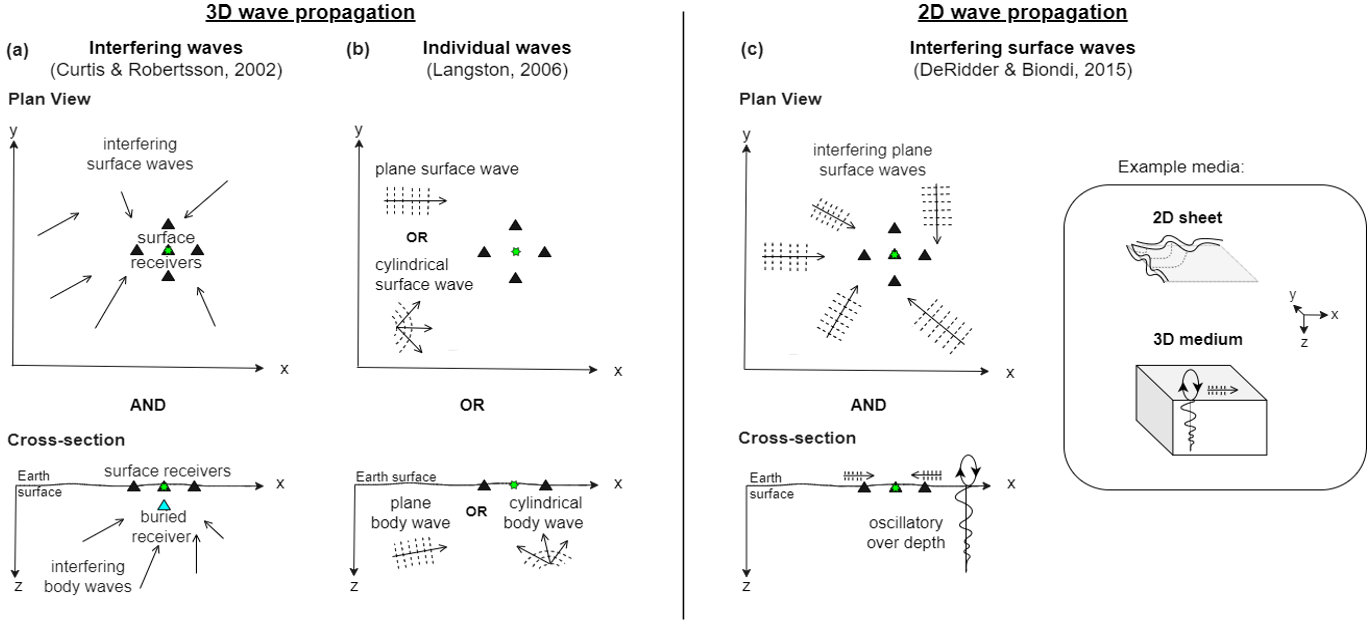
\includegraphics[width =\linewidth]{../Figures/acquisition_new26_07.png}
		\caption{Schematic of acquisition geometries and physical assumptions made for different gradiometry types in plan view and cross-section view. Receivers are denoted by triangles and the configurations requiring the minimum number of receivers are shown to estimate gradients via classical finite difference around the central point (green star) with receivers recording translational motion. (a) The left column shows principles of volumetric wavefield gradiometry as proposed by (\cite{curtis2002volumetric}): with a 3D receiver acquisition, second horizontal and vertical wavefield derivatives are approximated at a central point. To calculate derivatives in x-, y- and z-direction, 3-component (3C) receivers are necessary. Arrows denote interfering waves coming from all directions and angles; all wave types can be included in the wavefield e.g., surface waves, body waves, scattered waves, etc.  (b) Middle column shows gradiometry for non-interfering waves as proposed by (\cite{Langston1}). Individual plane or cylindrical waves can arrive from any direction at the receiver array. Receivers are used to estimate first horizontal derivatives of the wave field quantity; the central point does not require a recording. Receivers can be (1C) or (3C) depending on which wave type is analysed. Rotational sensors at the free surface allow for direct measurement of first derivatives (\cite{schmelzbach2018advances}; \cite{sollberger2020seismological}). (c) Right column shows principles of surface wave gradiometry as proposed by (\cite{de2015near}) where second order horizontal wavefield derivatives are approximated. This gradiometry type assumes a wavefield composed of interfering surface plane waves in a 3D medium, or Lamb waves in a 2D sheet (inset). }
		\label{fig:gradio_types}
	\end{figure}


	
	The latter applications of surface wave WEI are based on the assumption that Rayleigh waves are the dominant wave type and that the 2D scalar Helmholtz wave equation describes the recorded wavefield adequately (\cite{de2015near}; \cite{cao2020near}). This is a significant approximation for seismic waves because the Helmholtz equation fails to describe general elastic wavefield dynamics. Since ambient noise recordings contain all kinds of interfering elastic wave types (such as surface waves themselves), the accuracy of subsurface material property estimates may be compromised. Nevertheless, \textcite{shaiban2022wavefield} used a synthetic 2D elastic ambient noise wavefield to show that the correct local dispersion curves for a layered, laterally heterogeneous model could be estimated from the relationship between spatial and temporal gradients in the Helmholtz equation.\\

	Surface wave WEI has been shown to require only a few minutes of ambient seismic noise recordings and rapid data processing after acquisition to produce useful phase velocity maps for the near-surface (at frequencies between 18 Hz to 24 Hz), and so shows promise for efficient field deployment and near-real time monitoring purposes for the shallow subsurface (\cite{cao2020near}). 
	%Phase velocity estimates can be made for each receiver station individually over an array deployment which delivers information on lateral changes in dispersion curves over the array. 
	By estimating phase velocity maps for narrow band-pass filtered wavefields over a broad frequency range (depending on the ambient noise spectrum), the latter authors showed that 3D images of a layered subsurface can be produced via inversion of local surface-wave dispersion curves for S-wave velocity ($V_{s}$) structure. 2D shear-velocity maps for several depth levels up to 50 m were obtained in a matter of seconds from the dispersion curve through depth inversion performed by mixture-density neural networks (MDN).
	%To decrease uncertainty and conserve information on lateral heterogeneities, a 3-D non-linear surface wave tomography method can be tested ((\cite{zhang1}); (\cite{zhang2})). 
	However, the quality of the 3D shear velocity models are not only dependant on the accuracy of the phase velocity data but also on the impact of density in the inversion process (\cite{ivanov2016impact}). Dispersion-curve inversion for $V_{s}$ generally uses predefined values for compressional-wave velocity ($V_{p}$) and density because their sensitivities to the phase velocity are much smaller than that of the S-wave velocity (\cite{foti2018guidelines}; \cite{pan2019sensitivity}; \cite{wu2020shear}). Such a-priori information on $V_{p}$ is commonly obtained from other measurements and density is often assumed constant (e.g. \cite{cao2020near}) or inferred from empirical relationships with compressional wave speed.
	% In the derivation of the forward function in layered media for Rayleigh wave dispersion curve calculation, density does however play a role in the form of ratios between depth layers ((\cite{thomas}); (\cite{knoploff})). 
	Unfortunately, vertical density variations have been shown to affect the inverted $V_{s}$ results, and the use of an inaccurate density background model can lead to false structures and overestimations in the $V_{s}$ result (\cite{ivanov2016impact}). Expanding surface wave WEI to estimate the density structure of the subsurface and to quantify the effect of density gradients on the phase velocity estimates could therefore improve $V_{s}$ models and seismic interpretation based on gradiometric methods.\\
	%By introducing neural networks into the mapping process from surface wave dispersion curves to 1D S-wave velocity depth profiles, 3D images of the subsurface could be produced in a matter of seconds (\cite{cao2020near}).


	
	%Starting from this so-called volumetric wavefield gradiometry (VWG) setup, several approximations in both wave physics and field acquisition geometries are made to arrive at the conventional 2D scalar wave equation which relies only on 1-component (1-C) sensors at the surface. 3D 3-C VWG is valid for all incoming wavefields whereas 2D 1-C Surface Wavefield Gradiometry (SWfG) assumes the wavefield traveling in a 2D surface plane and no energy coming from depth. Given that 3D wavefield information from buried receivers or borehole data is not widely available, we usually do not have any knowledge about depth derivates of the wavefield. 2D field setups with standard 1-C receivers are still the norm in seismic acquisition which makes SWG more accessible to use, hence SWG is further investigated in this work. 

	
	%Most efforts aimed at estimating density have been performed with means of Full Waveform Inversion (FWI) (insert REFS).

	%discuss frequency dependance in density recovery, no influence of deeper layer. so are we actually getting local surface density? more targeted tests needed 

	%%this introduces paragraph where we measure pressure because direct sensitvity to pressure, in compressional part of wave propagation

	
	In this study we investigate whether it is possible to estimate subsurface density on the basis of gradiometric surface wave WEI using ambient seismic noise. Both the accuracy in wave amplitude and shape are important considerations in gradiometric methods, and density heterogeneities were found to have an influence on both (\cite{plonka2016imprint}; \cite{blom2017synthetic}). Hence, we expect to have sensitivity to the effect of density contrasts by using data that record variations in wavefield amplitudes and phases. \\

	In the Helmholtz formulation, which has been used in previous surface wave WEI studies, the wave equation does not exhibit an explicit sensitivity to density. In elastic media, the scalar Helmholtz wave equation is valid for surface waves only in laterally homogeneous medium. In a realistic scenario, the subsurface is heterogeneous with \DIFaddbegin \DIFadd{velocity and }\DIFaddend density varying both laterally and with depth. \DIFaddbegin \DIFadd{In heterogeneous media, the superposition of multipathing surface waves propagates with a velocity that does not only depend on the structural properties of the underlying medium, but also on the distribution of amplitudes of the interfering wavefield (\mbox{%DIFAUXCMD
\cite{wielandt2}}\hskip0pt%DIFAUXCMD
). }\DIFaddend This implies that the Helmholtz wave equation is not a valid description for surface wave propagation \DIFdelbegin \DIFdel{(\mbox{%DIFAUXCMD
\cite{wielandt2}}\hskip0pt%DIFAUXCMD
) }\DIFdelend and is likely to influence the accuracy of phase velocity estimates made via 2D scalar WEI. \DIFaddbegin \DIFadd{In practice, if the medium is only smoothly heterogeneous, the Helmholtz equation is usually considered to be approximately valid for each surface wave mode separately. }\DIFaddend Seismic surface waves are however commonly approximated by acoustic waves, by assuming that the wavefield is purely dilatational and is dominated by pressure wave propagation. The acoustic approximations neglects mode conversions and the directivity of scattering from a point heterogeneity  (\cite{wielandt2}), simplifying the mathematical model of wave propagation considerably. \\

	The scalar Helmholtz wave equation more accurately describes waves in acoustic media than in elastic media. In fact in the acoustic case, the main simplification made in the derivation of the conventional scalar wave equation is that density is assumed to be constant across the local receiver array. To describe a more complex, physically more realistic medium, a variable density assumption can be made, which allows the acoustic medium to be described by a so-called full acoustic wave equation. The full acoustic wave equation was initially derived by \textcite{bergmann1946wave} to define conditions under which density gradients in the atmosphere and large bodies of water should not be neglected in the governing wave equation formulation of sound pressure. The formulation of the full acoustic wave equation considered in that work assumes that gravity effects are negligible, and allows for density changes caused by either temperature gradients or changes in chemical composition of the material (\cite{bergmann1946wave}).\\ %In the solid Earth, density can generally be assumed to be scaled with velocity for temperature induced perturbations, whereas chemical changes in rock composition can cause density and shear wave speed heterogeneities to be anti-correlated (\cite{plonka2016imprint}). 

	%(\cite{tarantola1984inversion}) writes that if there is a diffractor at a point in space (a point perturbation of bulk modulus or of density), a diffracted pressure field at that point can be correlated with the incident wave field. This suggests that measuring the pressure field can be directly related to density perturbations and allows to infer unambiguous information about subsurface density.\\
	% shortcoming
	In this paper we analyse wavefield sensitivities to subsurface density contrasts via WEI of the full-acoustic wave equation where density is treated as a variable. We expect the full acoustic formulation may allow us to analyse the role of density independently from wave speed. To test this hypothesis, we initially consider waves propagating through an acoustic medium so that the physics of the used wave equation are consistent with the physics of the medium. We show that it is possible to invert for density on the basis of full acoustic WEI and compare the effect of using the Helmholtz and full acoustic equation on phase velocity results in 3D acoustic media. We then analyse whether the procedure is applicable to elastic media despite the concomitant severe approximations to the complex elastic wavefield physics. In elastic media, particle velocity is the natural wavefield observable rather than pressure, but we show that measuring pressure is necessary in order to relate the full acoustic wave equation approximation to the elastic case and to formulate an inverse algorithm that is explicitly sensitive to density. We then investigate whether volumetric gradiometry better lends itself to invert for density using the physically more representative full elastic wave equation at the free surface. By expressing the full elastic wave equation both in terms of pressure and displacement at the free surface we establish that a direct sensitivity to density exists and that density can be estimated.\\

	%In elastic media however, particle velocity is the natural wavefield observable, not pressure. The pressure at the free surface is predominantly composed of horizontal derivatives of surface wave displacement  \\

	% We aim to analyze the physical accuracy of wavefield gradiometry by addressing one of the approximation steps that is made in order to arrive at the conventional 2D scalar wave equation: the assumption that density is constant across the local array.  
	% An acoustic approximation is valid for elastic P-waves in a homogeneous, isotropic medium, but is compromised in heterogeneous or anisotropic media due to P-to-S conversions
	%Ambient noise is dominated by surface waves that are predominantly controlled by S-wave motion. So in such a wavefield we are trying to fit a wave equation valid for pressure wave motion only... 
	%Therefore, it also poses a severe approximation to the complex elastic wavefield. We do expect this formulation to allow us to analyse the potentially independant role of density in elastic media. \\
	%  The only approximation that depletes information is due to the 2D acquisition.
	 %Both the accuracy in wave amplitude and shape are important considerations in gradiometric methods, and density was found to have an influence on both ((\cite{plonka2016imprint});(\cite{blom2017synthetic})).
	% Hence we expect the neglect of density in the scalar wave equation formulation to impact phase velocity results obtained via gradiometric 2D surface wave WEI negatively. After demonstrating feasibility, we analyse whether the procedure is applicable to elastic media despite the approximations in physics.\\
	%Density, meanwhile, is poorly constrained, due to the sensitivity of the measurements to contrasts in density rather than the parameter itself, and due to the fact that of the imaged quantities, it has the smallest imprint on the wavefield, making it more sensitive to data or modelling errors. direct quote (Blom et al. 2020) ++ bring in Plonka piblications

	 
	
	%Given that acoustic surface waves in elastic media are known to have sensitivities to density structure, we expect that the proposed iterative density and phase velocity inversion process could be applicable to wavefields that are dominated by these wave types. 

	%\end{multicols}

	% so far, how we got density .. FWI, FWI& gravity, etc...
	% viscoacoustic FWI for density (\cite{operto_miniussi} and \cite{prieux_virieux}) for density


	
	

	
	\section{Wave Theoretical Background} \label{sec:theory}
	%\begin{multicols}{2}

	Density plays a different role in elastic and acoustic media. To illustrate, we compare the derivations of the respective governing wave equations from Newton's $2^{ nd}$ Law 
	\begin{align}\label{eq:newton2nd}
		\shoveright  \shoveright  \shoveright  \shoveright \shoveright \shoveright  
		\shoveright  \shoveright  \shoveright  \shoveright \shoveright \shoveright  \shoveright  \shoveright  
		\nabla  \cdot  \bm{\sigma} \:	+ \: \bm{f} \: &= \:   \rho \: \partial_{t}^{2} \: \mathbf{u}
	\end{align}
	where $ \bm{\sigma} = \sigma_{kl}$ is the stress tensor assuming k and l to range from 1 to 3 (for the x, y and z directions), $\rho$ is subsurface density, $\bm{f}$= $ [f_{x}, f_{y}, f_{z}]^{T}$ is the distribution of applied body forces, \textbf{u} = $ [u_{x}, u_{y}, u_{z}]^{T}  $ the observed wave field quantity of displacement or particle velocity, and $\nabla = [\partial_{x}, \partial_{y}, \partial_{z}]^{T}$ in three dimensional media. \DIFaddbegin \DIFadd{The wave field quantity }\textbf{\DIFadd{u}} \DIFadd{is defined with respect to a reference state in which the medium is in equilibrium under gravity. }\DIFaddend It is well known that in isotropic elastic media and small displacements, Hooke's law allows stress to be expressed in terms of the strain tensor $\bm{\epsilon}$ (where element  $\epsilon_{xy} = \partial_{x}u_{y}+\partial_{y}u_{x}$ and similarly for other elements) and the Lam${\'e}$ parameters $\lambda$ and $\mu$. This relationship can then be substituted in equation (\ref{eq:newton2nd}). Similarly for acoustic media, however the equations are then simpler because the shear modulus $\mu = 0$:
	%  \[
	%\begin{array}{ll}
	%	\text{Elastic Media:}\\
	%	\text{Acoustic Media:}
	%\end{array} \left\{
	%\begin{array}{ll}
	%	\mbox{\begin{equation}
			%			\Delta \cdot (\lambda \: tr(\bm \epsilon) \: I + 2\mu \bm\epsilon)  \:	+ \: \bm{f}   \: = \:  \rho  \: \partial_{t}^{2} \: \mathbf{u} \:, \label{eq2a} 
			%		  \end{equation}}\\
	%		\mbox{\begin{equation}
			%				\Delta \cdot (\lambda \: tr(\bm \epsilon) \: I ) 	\:	+ \: \bm{f} 			   \: = \:  \rho  \: \partial_{t}^{2} \: \mathbf{u} \:. \label{eq2b}
			%	\end{equation}}\\
	%\end{array}
	%\right.
	%\]
	\begin{subequations}
		\begin{align}
			\shoveright  \shoveright  \shoveright  \shoveright \shoveright \shoveright  \shoveright  \shoveright   
			\nabla \cdot (\lambda \: tr(\bm{\epsilon}) \: I + 2\mu \bm{\epsilon})  \:	+ \: \bm{f}   \: &= \:  \rho  \: \partial_{t}^{2} \: \mathbf{u} \: \quad \quad \quad \quad \text{in elastic media} 
			\label{eq2a} \\		
			\shoveright  \shoveright  \shoveright  \shoveright \shoveright \shoveright  \shoveright   \shoveright  				   
			\nabla \cdot (\lambda \: tr(\bm{\epsilon}) \: I ) 	\:	+ \: \bm{f} 				   \: &= \:  \rho  \: \partial_{t}^{2} \: \mathbf{u} \: \quad \quad \quad \quad \text{in acoustic media} 
			\label{eq2b}
		\end{align}
	\end{subequations} %\mbox{} \\
	where tr() is the trace operator. By substituting expressions for elements of $\bm{\epsilon}$ into equations (\ref{eq2a}) and (\ref{eq2b}) we obtain the familiar 3D elastic wave equation for isotropic, locally homogeneous media, and a description of pressure wave propagation in terms of the wave field quantity \textbf{u}, respectively:
	\begin{subequations}
		\begin{align}
			\frac{(\lambda + 2\mu)}{\rho} \: [\nabla (\nabla \cdot \bm{u})] \: - \: \frac{\mu}{\rho} \:[\nabla \times (\nabla \times \bm{u})]  +\frac{\bm{f}}{\rho}	\: &= \: \partial_{t}^{2} \: \mathbf{u} \: \quad \quad \quad \quad \text{in elastic media}
			\label{eq3a}   \\
			\frac{\lambda}{\rho} \: [\nabla (\nabla \cdot \bm{u})] +\frac{\bm{f}}{\rho}  \: &= \: \partial_{t}^{2} \: \mathbf{u} \:  \quad \quad \quad \quad \text{in acoustic media} 
			\label{eq3b} 
		\end{align} 
	\end{subequations} %\mbox{} \\
	In this paper we focus on the case in which we would like to use ambient seismic noise, so we assume an absence of strong local sources in the area of wavefield recording and henceforth omit source term $\bm{f}$. In acoustic media, the first Lam${\'e}$ parameter $\lambda$ is the acoustic bulk modulus ${K_{a}}$, whereas the bulk modulus in elastic media is $K_{e} = \lambda + \frac{2}{3} \mu$. In elastic media, density is expressed only in combination with the Lam${\'e}$ parameters within the terms equating to P-wave velocity $v_{P,e} = \sqrt{(\lambda + 2\mu) / \rho}$ and S-wave velocity $v_{S,e} = \sqrt{\mu / \rho}$ respectively in equation (\ref{eq3a}), and similarly for acoustic media. This implies that while it may be possible to estimate the velocities from waveform data $\bm{u}$, it will not be possible to discriminate the Lam${\'e}$ parameters from the density since any velocity value can be fit by any density given a suitable choice of $\lambda$ and $\mu$. \mbox{} \\ \mbox{} \\
	In acoustic media, we often measure pressure $P$ rather than wavefield displacement or particle velocity. The particle velocity field can then be estimated from this measured pressure field (\cite{robertsson2002rough}; \cite{amundsen2005rough}). Pressure is directly related to the divergence of the wavefield displacement \textbf{u} via the equality $P = K_{a} \: \nabla \cdot \bm{u} $, where $K_{a}$ is the bulk modulus in acoustic media\DIFdelbegin \DIFdel{and $\nabla = [\partial_{x},\partial{y},\partial_{z}]^{T}$}\DIFdelend . By applying a divergence operator to both sides of the acoustic wave equation (\ref{eq3b}) it is possible to express an explicit sensitivity of measurements of pressure $P$ to density $\rho$:
	%\begin{align}\label{eq:press_ac}
	%	\shoveright \shoveright \shoveright \shoveright \shoveright \shoveright  \shoveright \shoveright  \shoveright  \shoveright  \shoveright \shoveright  \shoveright  \shoveright \shoveright %\shoveright  \shoveright  \shoveright
%		P = K_{a} \: \nabla \cdot \bm{u} 
%	\end{align}%$P = K_{a} \: \nabla \cdot \bm{u} $,
	\begin{align}
	\shoveright  \shoveright  \shoveright  \shoveright \shoveright \shoveright  \shoveright  				   
	\DIFaddbegin \DIFadd{\quad }\DIFaddend \: \nabla \DIFdelbegin %DIFDELCMD < & %%%
\DIFdelend \cdot \bigg(\frac{K_{a}}{\rho} [\nabla (\nabla \cdot \bm{u})] \bigg)\DIFaddbegin &   \DIFaddend \: \:\:\:\: \DIFdelbegin \DIFdel{\:\: \:\:\:\: \:\: \: \: \: }\DIFdelend = \: \: \:\nabla \cdot \partial_{t}^{2} \bm{u}  \label{eq4} \\
	%DIF < \:\: \nabla \cdot \bigg(\frac{1}{\rho} \nabla P\bigg)                           \:  \:\:\:\:\:\:\:\:\:\:\: \:  &\: = \: \:\frac{1}{K_{a}} \:  \partial_{t}^{2} P  \\
		\DIFaddbegin \DIFadd{\quad \: }\DIFaddend \Rightarrow \DIFdelbegin %DIFDELCMD < & %%%
\DIFdelend \:\: \DIFaddbegin \DIFadd{v_{P,a}^{2} }\DIFaddend \:\DIFdelbegin \DIFdel{\quad  }\DIFdelend \: \DIFdelbegin \DIFdel{\: }\DIFdelend \rho \: \nabla \cdot \bigg( \frac{1}{\rho} \nabla P \bigg)\DIFaddbegin &  \DIFaddend \:\:\DIFdelbegin \DIFdel{v_{P,a}^{2} }\DIFdelend \:\:\:   \DIFdelbegin \DIFdel{\: \:  }\DIFdelend = \: \: \: \: \: \: \: \: \: \: \partial_{t}^{2} P  \label{eq6}
	\end{align}
	where in equation \eqref{eq6} we have used the definition of P wave velocity in acoustic media $v_{P,a} = \sqrt{K_{a}/\rho}$. Since density appears separately from P-wave velocity and has a different relationship to the measurable right hand side of equation (\ref{eq6}), we expect a potentially distinguishable density signature in seismic waves travelling through heterogeneous media in which the spatial derivative of density on the left is non-zero.\\

	% Similarly, changes in density are related to dilatational changes to the medium caused by pressure waves. A pressure change corresponds to a change in volume of the medium and is proportional to the divergence of the displacement field. At the traction-free free surface the divergence can be expressed in terms of the Lame parameters and the horizontal wavefield derivatives thanks to the relationships between first-order derivatives described in (\cite{curtis2002volumetric}). Expression can be found in (\cite{maeda2016reconstruction}, \cite{shapiro2000energy}).

	\textcite{cance2015validity} show how elastic and acoustic wave equations can be related in an isotropic, homogeneous domain for an explosive isotropic source emitting only P-waves. In such a case, the curl of the wavefield is equal to zero ($\nabla \times \bm{u} \: = \: 0$) and any vector field such as the displacement $\bm{u}$ or the particle velocity field $\bm{v}= \partial_{t} \bm{u}$  can be derived from a potential $\Phi$ (\cite{kaufman2000acoustic}). The potential $\Phi$ may be chosen as in \textcite{cance2015validity} to be
	\begin{align}\label{eq:potential_}
		\shoveright \shoveright \shoveright \shoveright \shoveright \shoveright  \shoveright \shoveright  \shoveright  \shoveright  \shoveright \shoveright  \shoveright  \shoveright \shoveright \shoveright  \shoveright  \shoveright
		\bm{u} \: &=\: \frac{1}{\rho} \: \nabla \Phi
	\end{align}
	where $\Phi$ is directly related to acoustic pressure via the relationship $\Phi = -2 P_{e}$ and where the pressure wavefield $P_{e}$ in elastic media is %(eq. \ref{eq:press_ac}) 
	\begin{align}\label{eq:press_el}
		\shoveright \shoveright \shoveright \shoveright \shoveright \shoveright  \shoveright \shoveright  \shoveright  \shoveright  \shoveright \shoveright  \shoveright  \shoveright \shoveright \shoveright  \shoveright  \shoveright
		P_{e} = -\frac{1}{2} K_{a} \nabla \cdot \bm{u}
	\end{align}
	Substituting equation (\ref{eq:potential_}) into equation (\ref{eq3a}) yields,
	%\begin{subequations}
	\begin{align}
		\shoveright  \shoveright  
		\frac{\lambda + 2 \mu}{\rho} \: \nabla \: \Big[  \nabla \cdot \bigg( \frac{1}{\rho} \nabla \Phi \bigg) - \frac{1}{\lambda + 2 \mu} \partial_{t}^{2} \Phi \Big] \:\DIFaddbegin \DIFadd{\: }\DIFaddend &= \: 0 \label{eq_el_ac1} \\ 
		\nabla \cdot \bigg( \frac{1}{\rho} \nabla \Phi \bigg) - \frac{1}{\lambda + 2 \mu} \partial_{t}^{2} \Phi \:\DIFaddbegin \DIFadd{\: }\DIFaddend & = \: \DIFdelbegin \DIFdel{c }\DIFdelend \DIFaddbegin \DIFadd{const }\DIFaddend \label{eq_el_ac2}
	\end{align} 
	%\end{subequations}

	Since equation (\ref{eq_el_ac1}) holds everywhere and so \DIFdelbegin \DIFdel{constant $c$ }\DIFdelend \DIFaddbegin \DIFadd{the constant }\DIFaddend is independent of position of the recording, and because the wave is absent (has zero energy) at infinity (\cite{kaufman2000acoustic}), equation (\ref{eq_el_ac2}) gives the potential equation in elastic media, 
	\begin{align} 
		\shoveright \shoveright \shoveright \shoveright \shoveright \shoveright	\shoveright \shoveright \shoveright	\shoveright
		\: \: \DIFaddbegin \DIFadd{c_{\omega}^{2} }\DIFaddend \: \DIFaddbegin \DIFadd{\: }\DIFaddend \rho \: \nabla \cdot \bigg(\frac{1}{\rho} \nabla \Phi \bigg) \: \:  \DIFdelbegin \DIFdel{c_{\omega}^{2} }\DIFdelend \:  &= \:  \partial_{t}^{2} \Phi  \label{eq_el_potential}
	\end{align}

	%closely resembling the full acoustic equation in acoustic media, only differing by their velocity expression and the recorded wavefield quantity. 
	\DIFdelbegin \DIFdel{which is the equation of }\DIFdelend \DIFaddbegin \DIFadd{where $c_{\omega}$ is the phase velocity at frequency $\omega$. Equation \eqref{eq_el_potential} describes }\DIFaddend acoustic wave propagation in elastic media \DIFdelbegin \DIFdel{, }\DIFdelend \DIFaddbegin \DIFadd{and is }\DIFaddend the elastic equivalent of equation \eqref{eq6} for acoustic media. \\

	The above equations show that different seismic observables interact differently with the subsurface: to isolate the effect of density from wave speed in elastic media on the basis of the full acoustic approximation or the elastic wave equation at the free surface, it is necessary to measure pressure instead of particle displacement or velocity (equations \ref{eq:potential_} to \ref{eq_el_potential}) because pressure implicitly includes a power of $K_{a}$ which changes the form of the respective equations. Classical seismometers only measure particle velocity, from which displacement can be calculated by time integrating the data, whereas elastic pressure is usually not observed on land. The expression for pressure is proportional to the divergence of the displacement (eq. \ref{eq:press_el}) which can be determined from four geophone recordings at the Earth's free surface using gradiometry (\cite{robertsson1999wavefield}; \cite{shapiro2000energy}; \cite{robertsson2002wavefield}). Given that stress is equal to zero across the free surface, the vertical derivative of the wavefield can be expressed in terms of horizontal derivatives. This results in the wavefield divergence taking a modified form that can be written in terms of the Lam${\'e}$ parameters and the horizontal wavefield components only \DIFdelbegin \DIFdel{$\nabla \cdot \bm{u} = (2 \mu/(\lambda + 2\mu)) \: \nabla_{H} \cdot \bm{u}^{H}$ }\DIFdelend \DIFaddbegin \DIFadd{$\nabla \cdot \bm{u} = (2 \mu/(\lambda + 2\mu)) \: \nabla_{H} \cdot \bm{u}_{H}$ }\DIFaddend where $\nabla_{H} = [\partial_{x}, \partial_{y}]^{T}$ and \DIFdelbegin \DIFdel{$\bm{u}^{H} = [u_{x}, u_{y}]^{T}$ }\DIFdelend \DIFaddbegin \DIFadd{$\bm{u}_{H} = [u_{x}, u_{y}]^{T}$ }\DIFaddend (e.g. \cite{maeda2016reconstruction}). However, calculating the divergence alone is not sufficient to estimate subsurface density as the density signal is contained in the full pressure measurement (eq. \ref{eq:press_el}).\\

	\textcite{edme2018seismic} suggest that it is possible to measure pressure directly at the free surface of an elastic medium with a land hydrophone. The land hydrophone is insensitive to the direction and angle of incoming waves which makes it predominantly sensitive to pressure fluctuations induced by ground-roll (more specifically, S-to P-conversions generated by upcoming S-waves) due to destructive summation of events at near vertical incidence angle. At the free surface of the Earth, elastic pressure $P_{e_{, FS}}$ can be written in terms of displacement in a 2D plane and its horizontal derivatives as (\cite{edme2018seismic})
	\begin{align}\label{eq:PRESS_edme}
		\shoveright \shoveright \shoveright \shoveright \shoveright \shoveright  \shoveright \shoveright  \shoveright  \shoveright  \shoveright \shoveright  
		P_{e_{, FS}} \: &=\: K_{e_{, FS}} \nabla_{H} \cdot \bm{u}\DIFdelbegin \DIFdel{^{H}  }\DIFdelend \DIFaddbegin \DIFadd{_{H}  }\DIFaddend \: \approx \: 0.37 \: K_{a} \nabla_{H} \cdot \bm{u}\DIFdelbegin \DIFdel{^{H} 
	}\DIFdelend \DIFaddbegin \DIFadd{_{H} 
	}\DIFaddend \end{align}
	where the elastic bulk modulus at the free surface is  $K_{e_{, FS}} = 2 \rho \: v_{S}^{2} \: (1- 4 \: v_{S}^{2}/3 \: v_{P}^{2}) $ \DIFaddbegin \DIFadd{and $v_{P}$ and $v_{S}$ are the local P- and S-wave velocities, respectively}\DIFaddend . The elastic pressure at the free surface can be related to acoustic pressure using $v_{P} = \sqrt{3} v_{S}$ \DIFaddbegin \DIFadd{for a Poisson solid}\DIFaddend . The measured pressure thus corresponds to the volume change caused by the dilatational part of surface wave propagation.\\ %Rayleigh waves exhibit a compressional wave motion that can be measured in the pressure field. That is however not the full description of the surface wave motion and probably subject to artefacts. Sensitivities of different wave types: In elastic media, we are measuring the pressure components of surface waves even though the assumption is valid only for P-wave propagation. \\

	Acoustic pressure caused purely by P-wave propagation in a non-rotational medium has a similar expression to elastic pressure at the free surface caused by the dilatational part of surface wave propagation. Surface waves can only be produced in a medium where rotation exists, and are generated by P- and S- wave interactions upon reflections and scattering at medium heterogeneities. Their propagation is mostly driven by S-waves which correspond to the purely rotational part of the wavefield. Nevertheless, Rayleigh waves do exhibit dilatational wave propagation that produces a measurable pressure field at the free surface. The full acoustic approximation is only valid for elastic P-waves in a homogeneous, isotropic medium, and is compromised in heterogeneous or anisotropic media due to P-to-S conversions. It thus does not describe a wave type that depends on body-wave conversions that are predominantly controlled by S-wave motion, even if only its compressional part is recorded. P-waves and the P component of Rayleigh waves therefore presumably interact differently with the medium and might exhibit different sensitivities to different subsurface parameters such as subsurface density. \textcite{cance2015validity} found that acoustic and elastic pressure are not the same for rough, heterogeneous media: a good agreement can only be achieved in homogeneous or weakly heterogeneous, smooth media. This suggests that in a realistic subsurface problem, inverting for the parameters on the basis of an acoustic approximation might be too approximate an approach to obtain sufficiently accurate information about elastic subsurface parameters by measuring pressure. We test this in what follows. \\
	%investigate whether, despite the approximation, measuring acoustic pressure is sufficient to gain information on subsurface density in elastic media. \\% Within their simulations, the pressure was however recorded within the medium and not at the free surface.\\ 
	%Elastic pressure at the free surface might be more closely related to acoustic pressure as suggested above.\\  %A measurement of pressure corresponds to the diagonal elements of the elastic stress tensor. Were we able to not only measure the diagonal elements of the stress tensor, but its full extent, it might be possible to estimate density from (\ref{eq:newton}) directly.

%	XXXX An elastic wavefield typically contains various wave types and can not be purely reduced to dilatational P-wave propagation. if we measure only dilatational wavefield of elastic field....\\

	In elastic media it is not strictly necessary to consider the acoustic approximation in order to isolate density by substituting pressure. If we introduce the free surface conditions
	\begin{align}\shoveright \shoveright \shoveright \shoveright \shoveright \shoveright 
		\partial_{z} u_{x} \: =& \: - \partial_{x} u_{z}\label{eq:FS_cond1}\\ 
		\partial_{z} u_{y} \: =& \: - \partial_{y} u_{z} \label{eq:FS_cond2}\\
		\partial_{z} u_{z} \: =& \: - \frac{v_{P,e}^{2} - 2v_{S,e}^{2}}{v_{P,e}^{2}} \: (\partial_{x} u_{x} + \partial_{y} u_{y})
		\label{eq:FS_cond3}
	\end{align}

	which express the fact that stress across the free surface must be zero, then equation \eqref{eq3a} can be written in a modified form that is valid at the free surface and in the absence of body forces:	
	\begin{align}\shoveright \shoveright \shoveright \shoveright \shoveright \shoveright 
		\partial_{z}^{2} u_{x} \: =& \: \frac{\partial_{t}^{2} u_{x} }{v_{S,e}^{2}} - \Big(\nabla_{H}^{2}u_{x} \Big) - 2\Big(1-\frac{v_{S,e}^{2}}{v_{P,e}^{2}} \Big) \partial_{x} (\nabla_{H} \cdot \bm{u}\DIFdelbegin \DIFdel{^{H}}\DIFdelend \DIFaddbegin \DIFadd{_{H}}\DIFaddend )\label{eq:FS_eq2a_1} \\ 
		\partial_{z}^{2} u_{y} \: =& \: \frac{\partial_{t}^{2} u_{y} }{v_{S,e}^{2}} - \Big(\nabla_{H}^{2}u_{y}  \Big) - 2\Big(1-\frac{v_{S,e}^{2}}{v_{P,e}^{2}} \Big) \partial_{y} (\nabla_{H} \cdot \bm{u}\DIFdelbegin \DIFdel{^{H}}\DIFdelend \DIFaddbegin \DIFadd{_{H}}\DIFaddend )\label{eq:FS_eq2a_2}\\
		\partial_{z}^{2} u_{z} \: =& \: \frac{\partial_{t}^{2} u_{z} }{v_{P,e}^{2}} + \Big(1-2\frac{v_{S,e}^{2}}{v_{P,e}^{2}} \Big) \nabla^{2}_{H}u_{z}
		\label{eq:FS_eq2a_3}
	\end{align}

	\DIFaddbegin \DIFadd{Even though a free-surface is usually referred to as the interface of a half-infinite elastic medium in contact with vacuum (\mbox{%DIFAUXCMD
\cite{robertsson1995comparative}}\hskip0pt%DIFAUXCMD
), free-surface conditions are a reasonable approximation on Earth given that the subsurface has elastic properties and the contact layer is air, which has low density. In the case of granular medium (such as regolith) or in heavy atmospheres, the free-surface condition would need to be updated with more appropriate constraints.}\\

	\DIFaddend By using a so-called Lax-Wendroff derivative centering technique (\cite{lax1964difference}; \cite{blanch1997modified}; \cite{curtis2002volumetric}), the first order vertical derivative can be correctly represented at the free surface by a finite difference approximation to horizontal spatial derivatives. Using a 3D receiver array as proposed in Fig. \ref{fig:gradio_types}(a) it then becomes possible to approximate all quantities necessary to estimate body wave velocities at the free surface. For example, a new expression can be derived for the vertical displacement component in eq. \eqref{eq:FS_eq2a_3} by using the free-surface condition \eqref{eq:FS_cond3} and the Lax-Wendroff corrected finite difference depth derivative:
	\begin{align} \shoveright \shoveright \shoveright \shoveright \shoveright \shoveright 
		\partial_{t}^{2} \: u_{z} \: =  \: v_{P,e}^{2} \: A_{z}(t) \: - \: v_{S,e}^{2} \: B_{z}(t)  
		\label{eq:freeSurfT}   
	\end{align} 
	where $A_{z}(t)$ and $B_{z}(t)$ are expressions containing finite difference approximations to derivatives of the wavefield
	\begin{align} \shoveright \shoveright \shoveright \shoveright \shoveright \shoveright 
		A_{z}(t)  	\: &= \:   \frac{2}{\Delta z} \big(\nabla_{H} \cdot \bm{u}\DIFdelbegin \DIFdel{^{H} }\DIFdelend \DIFaddbegin \DIFadd{_{H} }\DIFaddend + [\partial_{z} u_{z}]_{fd} \big) \: - \: \nabla^{2}_{H} u_{z} \label{eq:Az} \\ 
		B_{z}(t) 	\: &= \:   \frac{4}{\Delta z} \big(\nabla_{H} \cdot \bm{u}\DIFdelbegin \DIFdel{^{H}}\DIFdelend \DIFaddbegin \DIFadd{_{H}}\DIFaddend \big) \: - \: 2\big(\nabla^{2}_{H}u_{z}\big)
		\label{eq:Bz}   
	\end{align}
	and where $\Delta z$ is the distance between the surface and the buried receiver, and $[\partial_{z} u_{z}]_{fd}$ is the first order finite difference depth derivative. The derivation of these expressions is described in detail in \textcite{curtis2002volumetric}, and herein, we only consider the constraints derived from the vertical displacement component as they were shown to better constrain body wave velocity estimates than those derived from horizontal components. Furthermore, inhomogeneous terms do not play a role in the vertical component at the free surface, making the expressions valid for any type of elastic medium without approximations (Appendix \DIFdelbegin \DIFdel{\ref{sec:AppendixC}}\DIFdelend \DIFaddbegin \DIFadd{\ref{sec:AppendixE}}\DIFaddend ). \\

	By using the relation $P=P_{e,FS}/0.37$ from eq. \eqref{eq:PRESS_edme}, acoustic pressure can be substituted into eq. \eqref{eq:Az} and \eqref{eq:Bz}:
	\begin{align} \shoveright \shoveright \shoveright \shoveright \shoveright \shoveright 
		A_{z}'(t)  	\: &= \:   \frac{2}{\Delta z} \big(\frac{1}{K_{a}}P + [\partial_{z} u_{z}]_{fd} \big) \: - \: \nabla^{2}_{H} u_{z} \label{eq:Az_new}  \\
		B_{z}'(t) 	\: &= \:   \frac{4}{\Delta z} \frac{1}{K_{a}}P \: - \: 2\big(\nabla^{2}_{H}u_{z}\big)
		\label{eq:Bz_new}   
	\end{align}

	Feeding the expressions for $A_{z}'(t) $ and $B_{z}'(t) $ into eq. \eqref{eq:freeSurfT} we obtain
	\begin{align} \shoveright \shoveright \shoveright \shoveright \shoveright \shoveright 
		%\partial_{t}^{2} \: u_{z}  -  \frac{2v_{P,e}^{2}}{\Delta z}  [\partial_{z} u_{z}]_{fd} + v_{P,e}^{2} \nabla_{H}^{2}u_{z} - 2v_{S,e}^{2} \nabla_{H}^{2}u_{z} \: &= \: \frac{1}{K_{a}} \Big( \frac{2v_{P,e}^{2}}{\Delta z}P - \frac{4v_{S,e}^{2}}{\Delta z} P\Big)\label{eq:freeSurf_P1} \\
		\partial_{t}^{2} \: u_{z}  +  v_{P,e}^{2} \Big[ - \frac{2}{\Delta z}  [\partial_{z} u_{z}]_{fd} +  \nabla_{H}^{2}u_{z} \Big] - 2 v_{S,e}^{2} \nabla_{H}^{2}u_{z}  \: &=  \: \: \: \frac{1}{\rho} \: \;  \Bigg[ \frac{1}{\Delta z} \Big( 2 - \frac{4v_{S,e}^{2}}{v_{P,e}^{2}}\Big) P\Bigg]
		\label{eq:freeSurf_P}   
	\end{align}
	Displacement measurements are all on the left-hand side and pressure measurements on the right-hand side of equation \eqref{eq:freeSurf_P}; in order to use this equation to constrain the velocities and density, both displacement and pressure must be measured simultaneously at the free surface. An explicit sensitivity becomes clear from eq. \eqref{eq:freeSurf_P} with density connecting the left- and right-hand sides of the equation linearly.\\

	\section{Gradiometric Methodology} \label{meth}
	\DIFaddbegin \DIFadd{Herein, we focus on the potential of gradiometric methods based on 2D surface arrays (e.g., \mbox{%DIFAUXCMD
\textcite{de2015near} }\hskip0pt%DIFAUXCMD
in Figure \ref{fig:gradio_types}c) and 3D volumetric arrays (e.g., \mbox{%DIFAUXCMD
\textcite{curtis2002volumetric} }\hskip0pt%DIFAUXCMD
in Figure \ref{fig:gradio_types}a)  to estimate density in addition to medium speed. We start outlining the 2D gradiometric methodology (Section \ref{methS}) for density inversion in light of equations \eqref{eq6} and \eqref{eq_el_potential}. These equations are naturally suitable for acoustic wave propagation, but subject to drastic approximations in elastic media. We investigate whether a practical 2D array setup, that limits the complexity of the wave equation (vertical wavefield gradients can not be determined) employed for WEI, yields sufficient information to estimate density in an acoustic medium where the physics fit the employed equations \eqref{eq6} and \eqref{eq_el_potential}, and extend the method to elastic media. We then test whether using a 3D array configuration (Section \ref{methV}) with an additional buried receiver, which makes it possible to use a physically more appropriate equation for elastic data (i.e., equation \ref{eq:freeSurf_P}), improves the density estimates in elastic media. The following sections are hence structured according to the gradiometric WEI approaches for density estimation based on free surface (Section \ref{methS}) and volumetric array recordings (Section \ref{methV}), respectively. 
	}

	\DIFaddend \subsection{Free surface arrays}\label{methS}
	In previous wavefield gradiometry studies performed with data from 2D receiver arrays on the Earth's surface, the role of density has been neglected. If density is assumed to be constant over space, equation (\ref{eq_el_potential}) reduces to the scalar Helmholtz wave equation, the 2D version of which is usually used as a basis for WEI where $\nabla$ is used as a 2D operator (\DIFdelbegin \DIFdel{$\nabla = \nabla^{H} = [\partial_{x}, \partial_{y}]^{T}$}\DIFdelend \DIFaddbegin \DIFadd{$\nabla = \nabla_{H} = [\partial_{x}, \partial_{y}]^{T}$}\DIFaddend ) and $\bm{x} = [x,y]^{T}$:
	\begin{align}\label{eq:helm}
		\shoveright \shoveright \shoveright \shoveright \shoveright \shoveright \shoveright \shoveright \shoveright \shoveright%\shoveright 
		\: \; \; c_{\omega}(\bm{x})^{2} \: \nabla^{2} \theta(\bm{x},t) &\: = \: \partial_{t}^{2}\theta(\bm{x},t)
	\end{align}
	Here, $\theta$ denotes any type of wavefield quantity (e.g., one component of the wavefield displacement or particle velocity field, or the pressure field) which varies as a function of horizontal position x and y and time $t$. This equation is a significant approximation to how seismic waves propagate in the Earth's subsurface: all 3D propagation of elastic body waves and of different types of surface wave, each associated with multi-component particle motions, are approximated by a single wave type propagating in 2D across the Earth's surface with a single independent component of particle motion. For example, in isotropic media Love waves are horizontally polarized and arrive most prominently on the transverse component, whereas the Rayleigh waves are polarized in a vertical plane and appear mainly on the vertical and radial components (\cite{shearer2019introduction}). In the case of ambient noise, we deal with complex wavefields arriving from multiple sources which makes it impossible to distinguish radial contributions from transverse contributions; Love and Rayleigh waves therefore interfere in the horizontal particle velocity field yet are treated as one wave type in the 2D scalar wave equation. On land, 1C geophone recordings are usually employed as gradiometric measurements, because Rayleigh waves typically dominate the ambient seismic noise field and predominantly excite vertical displacements. A similar argument applies to Scholte waves which travel along the water-seabed interface. And since surface waves predominantly travel across the Earth's surface and have a dominant mode number, they are commonly approximated by superpositions of dispersive, single-mode plane waves that each satisfy the 2D scalar wave equation. \\%Surface waves are highly dispersive in inhomogeneous media, meaning that different frequencies travel at different speeds.\\

	In order to improve the suitability of the Helmholtz approximation for surface waves, the wavefield is usually first filtered around a fixed frequency $\omega$. WEI then proceeds by estimating all spatial and temporal derivatives in equation (\ref{eq:helm}) given measurements of a passing wavefield made on a dense array. Thereafter the equation can be solved for the phase velocity $c_{\omega}$. Nevertheless, the series of approximations above degrades the estimates of surface wave velocity.\\ 

	%and which entails that their propagation does more closely resemble the 2D scalar wave equation than other wave types travelling in elastic media. They can thus be approximated by a superposition of single-mode plane waves that each satisfy the 2D scalar wave equation. 
	In acoustic media however, the Helmholtz wave equation may be a reasonable model of wave propagation because the only approximation made in governing physics is that density is assumed to be locally constant across the array of receivers used to estimate spatial derivatives in $\nabla P$. To account for a spatial variability in subsurface density, we consider the full acoustic wave equation in the time domain:
	% In the discussion we return to the issue of whether or how this relates to gradiometry in elastic media.
%	This section sets up an inverse problem to estimate density in an acoustic medium on the basis of gradiometry measurements. 

	\begin{align}\label{eq:FA}
		\shoveright \shoveright \shoveright \shoveright \shoveright \shoveright \shoveright \shoveright %\shoveright 
		\; \; \; \nabla \cdot \bigg( \frac{1}{\rho(\bm{x})} \nabla P(\bm{x},t) \bigg) &\: = \: \frac{1}{\rho(\bm{x}) \: c_{\omega}(\bm{x})^{2}} \: \partial_{t}^{2} P(\bm{x},t)
	\end{align}

	The full acoustic wave equation represents the underlying physics that relates phase velocity $c_{\omega}$ and density $\rho$ to dilatational wavefield observations where pressure $P$ is used as wavefield quantity $\Phi$. In acoustic media, equation (\ref{eq:FA}) captures the full physics whereas it is only an approximation of wave propagation in elastic media. To perform WEI on the basis of the full acoustic wave equation in elastic media, we need to compute the pressure wavefield P from equation \eqref{eq:press_el} and substitute the resulting potential $\Phi = K_{a} \nabla \cdot \bm{u}$ into equation (\ref{eq_el_potential}) where \DIFdelbegin \DIFdel{$\bm{u} = \bm{u}_{H} = [u_{x}, u{y}]$ and $\nabla = \nabla^{H} = [\partial_{x}, \partial_{y}]$}\DIFdelend \DIFaddbegin \DIFadd{$\bm{u} = \bm{u}_{H}$ and $\nabla = \nabla_{H}$}\DIFaddend .\\

	Using the foundation of the full acoustic wave equation we set up an inversion process to estimate both velocity and density from gradiometric measurements. We first parametrize the system in order to remove non-linearity in these forward relations. We simplify the form of equation (\ref{eq:FA}) by introducing parameters $g(\bm{x})$ and $h(\bm{x})$ that vary as a function of horizontal position: \\
	\begin{align}
		h(\bm{x}) \: &= \: \frac{1}{K(\bm{x})} \: = \: \frac{1}{\rho(\bm{x}) c_{\omega}(\bm{x})^{2}} \\  
		g(\bm{x}) \: &= \: \frac{1}{\rho(\bm{x})}
	\end{align}

	The full acoustic wave equation then becomes
	\begin{align} \label{eq:para}
		\shoveright \shoveright \shoveright \shoveright \shoveright \shoveright \shoveright \shoveright 
		\; \; \; \nabla g(\bm{x}) \nabla P(\bm{x},t) &\: = \: h(\bm{x}) \: \partial_{t}^{2} P(\bm{x},t)
	\end{align}
	%which we then discretize on a horizontal,
	We rely on accurate knowledge of second order spatial gradients of pressure which can not be measured directly in the field. We calculate these gradients discretely using finite differences which are based around Taylor series expansions (\cite{curtis2002volumetric}). We discretize equation (\ref{eq:para}) on a horizontal, regularly spaced receiver grid at the surface (Fig. \ref{fig:gridFD}a) using classical central finite differences (FD) after (\cite{Geiger2003FiniteDM}) to approximate the derivatives. Discretizing with the FD method does not require regular grids if we adopt a generalized FD scheme after (\cite{liszka1980finite}; \cite{huiskamp1991difference}; \cite{gavete2003improvements}), however in our case receiver spacing $\Delta x$ and $\Delta y$ in x and y directions respectively are constant and equal, and indices i and j define receiver locations where i ranges from [0,M] and j ranges from [0,N]. We formulate the discretized expression and rearrange the terms isolating the model parameter $g_{i,j}$ that contains information about subsurface density only:  
	%In gradiometry, we rely on accurate wavefield gradient information in order to invert for the medium's physical parameters. At the surface of the Earth, first order spatial derivative terms can be directly measured by rotational sensors (\cite{}). Distributed acoustic sensors measure the strain rate which can be related to the first-order spatial derivative of the strain. Usually DAS can provide only single axial strain measurement which are not adequate to characterize the full elastic wavefield.  only record Pressure gradient sensors for first order derivatives do exist (\cite{}). Second-order spatial gradients however are not directly measurable in the field, but can be calculated on dense receiver grids by using the discrete Finite Difference method.


	\begin{equation}
		%\shoveright \shoveright \shoveright
		\begin{split} \label{discr}
		&\frac{1}{2 \Delta x^{2}} \Big[P_{[0,-]}^{n}  \: g_{[i,j-1]} + P_{[-,0]}^{n}  \: g_{[i-1,j]}  \\ 
	    &+ P_{[\pm,\pm]}^{n}  \: g_{[i,j]} + P_{[+,0]}^{n}  \: g_{[i+1,j]}  + P_{[0,+]}^{n}  \: g_{[i,j+1]} \Big]  
		\: = \: h_{[i,j]} \left[ \frac{ P^{n+1}_{[i,j]} - 2P_{[i,j]}^{n} + P^{n-1}_{[i,j]} }{\Delta t^{2}} \right] 
		\end{split}
	\end{equation}

	where $P_{[0,-]}^{n} $ and $P_{[0,-]}^{n} $ are written similarly to
	\begin{align}
		P_{[0,+]}^{n} 	  & \: = \: P_{[i,j+1]}^{n}  - P_{[i,j]}^{n}    \label{d1} \\
		P_{[+,0]}^{n}  	  & \: = \: P_{[i+1,j]}^{n}  - P_{[i,j]}^{n}  \label{d2}
	\end{align}
	and 
	\begin{align}
	P_{[\pm,\pm]}^{n}  & \: = \: P_{[0,-]}^{n}  + P_{[-,0]}^{n}  + P_{[0,+]}^{n}  + P_{[+,0]}^{n} \label{d3} \\ \nonumber 
	\end{align}

	\begin{figure}[H] 
	\begin{subfigure}[c]{0.49\textwidth}
		\centering
		\subfloat[]{\includegraphics[width =0.9\textwidth, keepaspectratio]{../Figures/DiscreitzationGrid.png}}
	\end{subfigure}
	%\hfill{}
	\begin{subfigure}[c]{0.49\textwidth}
		\centering
		\subfloat[]{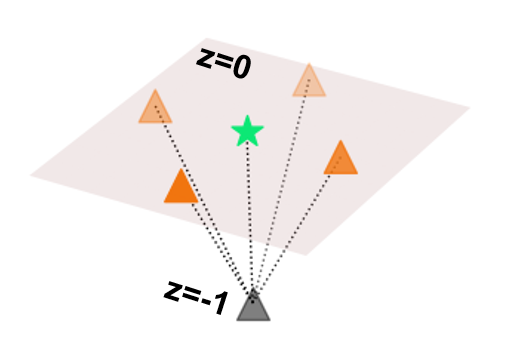
\includegraphics[width = 0.6\textwidth, keepaspectratio]{../Figures/buriedREC.png}}
	\end{subfigure}
	%\centering 
	%\captionsetup{width=\linewidth}
	%\includegraphics[width =0.45\textwidth]{DiscreitzationGrid.png}
	\caption{(a) Discretization of wavefield derivatives using a surface receiver grid, shown in plan view on the x-y plane. Receivers are marked by triangles (internal stations in blue, border stations in red). The grid has N rows in y-direction and M columns in x-direction. The pressure field $P$ is recorded at each receiver position [i,j]. The classical second order finite difference stencil of receivers is represented by the cross-shape (orange), using which the second order derivative of the wavefield is estimated at the central point marked by the star symbol (green). (b) shows the corresponding buried receiver (grey) at 1m below the surface that is used for volumetric gradiometry across the finite difference cross-shaped stencil.  }
	\label{fig:gridFD}	
	\end{figure}

	Equation \eqref{discr} can be written in matrix form
	\begin{align}
	\shoveright \shoveright \shoveright \shoveright \shoveright \shoveright \shoveright \shoveright \shoveright \shoveright \shoveright \shoveright \shoveright \shoveright \shoveright
 			 \mathbf{A} \; \mathbf{g}\DIFdelbegin \DIFdel{_{est} }\DIFdelend \DIFaddbegin \DIFadd{^{est} }\DIFaddend &\: = \: \mathbf{d}
	\end{align}
	where matrix \textbf{A} has dimensions [$R \times R \times n_{t}$] with R being the number of parameters over the receiver grid ($R=M \times N$) and $n_{t}$ the number of data in the time series. \textbf{A} contains purely observed data consisting of the pressure differences (equations \ref{d1} to \ref{d3}) and is banded and square [$R \times R$] for each time step $n$ in the time series of the signal. Vector $ \mathbf{g^{est}} = [g_{[0,0]}, g_{[1,0]},..., g_{[M,N]}]^{T}]$ is the parameter vector of dimension [$R \times 1$] to be estimated, and $\mathbf{d}$ is an observed data vector of dimension $[R \times n_{t}]$ that contains time derivatives of the recorded pressure field $P_{i,j}$ multiplied by terms $h_{i,j}$ (right-hand side of eq. \ref{discr}). Equally accurate calculations of derivatives at the corners and boundaries of the array are not possible since neighbouring receivers are not available in all directions so the full cross-shaped finite difference stencil (Fig. \ref{fig:gridFD}) can not be used and is depleted to a stencil formed by two or three adjacent stations only. %By only drawing on measurements from two or three neighbouring stations, the stencils becomes one-sided in the direction of available information which depletes the accuracy of the second order derivative estimate. % expand on that we dont want forward discretization because then we are dealing with a larger stencil, more averaging... and also less accuracy...? 
	We therefore introduce a weighting matrix $\mathbf{W}$ that gives less weight to information from corner and boundary points of the receiver grid which are likely to provide less accurate constraints than the internal receivers. For corner and border receivers we chose a weighting factor very close to zero to minimize the impact on results while still maintaining the invertibility of matrix $\mathbf{A}$. Consequently, density estimates are evaluated only at internal receivers. \\

	Since the density information is contained in both parameter vector $\mathbf{g^{est}}$ and the vector $\mathbf{d}$ through parameter vector $\mathbf{h}= [h_{[0,0]}, h_{[1,0]},..., h_{[M,N]}]^{T}]$, prior information is given in the form of an initial reference model for $\mathbf{h}$ which we call  $\mathbf{h}^{init}$:
	\begin{equation}
		\mathbf{h}^{init} \: = \: \frac{1}{\bm{\rho}_{ _{init}} \: \bm{c}_{\omega,_{ init}} }
	\end{equation}
	So as not to bias the inversion towards a heterogeneous solution, we chose a homogeneous reference for density $\rho_{ _{init}}$. The reference model  $c_{\omega,_{ init}}$ for phase velocity is obtained from an initial wave equation inversion using the standard scalar Helmholtz wave equation formulation \eqref{eq:helm} following the methods of \textcite{de2015near} and \textcite{cao2020near}. 
	%The absolute value for the initially constant density reference model could then be derived from the mean of the Helmholtz velocity result via the Gardener's relationship.
	To stabilise the inverse problem we introduce generalized Tikhonov regularization:
	\begin{align}
	\shoveright \shoveright \shoveright \shoveright  \shoveright \shoveright \shoveright \shoveright \shoveright \shoveright
	\: \:	[\bm{W} \bm{A} + \Theta_{d} \bm{I}] \; \bm{g}^{est} &\: = \: [\bm{d} + \Theta_{d} \bm{g}^{init}]
	\end{align}
	Damping term $\Theta_{d}$ controls how strongly the solution is drawn towards the homogeneous reference model $\bm{g}^{init}$ \DIFaddbegin \DIFadd{and has the same dimensions as matrix $\bm{A}$}\DIFaddend . We then find the least-squares solution for parameters $\bm{g}^{est}$ that contain the density information
	\begin{align} \label{eq:regul}
		\shoveright \shoveright \shoveright \shoveright  \shoveright \shoveright \shoveright \shoveright \shoveright \shoveright
		\: \:	\bm{g}^{est} &\: = \: [ \Sigma_{n=1}^{n_{t}} \: (\hat{\bm{A}}_{n}^{T}\hat{\bm{A}}_{n})^{-1} \: \hat{\bm{A}}_{n}^{T} ] \; [ \Sigma_{n=1}^{n_{t}} \: \hat{\bm{d}}_{n}] \:
	\end{align}
	where $\hat{\bm{A}} = [\bm{W}\bm{A}, \Theta_{d} \bm{I}]^{T}$ and $\hat{\bm{d}} = [\bm{d}, \Theta_{d} \bm{g}^{init}]^{T}$.
	After one iteration solving for $\bm{g}^{est}$, we obtain a first approximation to density that we note $\bm{g}'$. Substituting this density approximation into equation \eqref{eq:FA}, we estimate phase velocity using gradiometric methods where we write the discrete finite difference form of equation \eqref{eq:FA} in terms of parameter $\bm{g}'$ and estimate the phase velocity via linear regression similarly to (\cite{de2015near}):
	\begin{equation}
		\begin{split} \label{eq:discr_c} 
			\frac{1}{2 \Delta x^{2}} \: \Big[ &g_{[0,-]}' P_{[i,j-1]}^{n} + g_{[-,0]}' P_{[i-1,j]}^{n}
			-  g_{[\pm,\pm]}' P_{[i,j]}^{n} \\
			&\quad \quad \quad \; \; + g_{[0,+]}' P_{[i,j+1]}^{n} + g_{[+,0]}' P_{[i+1,j]}^{n} \Big] \; c_{\omega,[i,j]}^{2}
			\: = \: \left[ \frac{ P^{n+1}_{[i,j]} - 2P_{[i,j]}^{n} + P^{n-1}_{[i,j]} }{\Delta t^{2}} \right]
		\end{split}
	\end{equation}
	where $g_{[-,0]}'$ and $g_{[0,-]}'$ are written similarly to
	\begin{align}
	g_{[+,0]}'     &= \frac{g'_{[i+1,j]}}{g'_{[i,j]}}+1 \: \label{ratio1} \\ 
	g_{[0,+]}'     &= \frac{g'_{[i,j+1]}}{g'_{[i,j]}}+1 \:  \label{ratio2}
	\end{align}
	and
	\begin{align}
	g_{[\pm,\pm]}' &= g_{[0,-]}' + g_{[-,0]}' +  g_{[+,0]}' +  g_{[0,+]}' \: \label{rho_coeffs}  \nonumber
	\end{align}


	In matrix form, equation \eqref{eq:discr_c} can be written
	\begin{align}
		\bm{J}' \: \bm{m}' &\: = \: \bm{d'}
	\end{align}
	where  $ \mathbf{m}' = [c_{\omega,[0,0]}^{2}, c_{\omega,[1,0]}^{2},..., c_{\omega,[M,N]}^{2}]^{T}$ is the parameter vector of dimension [$R \times 1$], $\mathbf{d'}$ is an observed data vector of dimension $[R \times n_{t}]$ that contains time derivatives of the recorded pressure field and coefficient matrix $\bm{J}$ of dimensions [$R \times R \times n_{t}$] contains  knowledge about the pressure wavefield gradients and density gradients from the full acoustic wave equation formulation. \DIFaddbegin \DIFadd{In the case of real data, where amplitude differences in the wavefield due to site effects or difference in sensors can impact the data, it might be necessary to impose the condition that medium parameters should not vary rapidly as a function of space (\mbox{%DIFAUXCMD
\cite{de2015near}}\hskip0pt%DIFAUXCMD
). This can be achieved by adding a damping term, i.e., penalizing the second order spatial derivatives in the from of a Tikhonov regularization. For the purpose of this paper, where we analyse synthetic data only and the problem is well constrained, equation \eqref{eq:discr_c} is solved by linear regression with a mean squared cost function, i.e., non-regularized least-squares WEI. }\DIFaddend Information about density obtained from equation \eqref{eq:regul} and the updated phase velocity estimates obtained by solving equation \eqref{eq:discr_c}\DIFdelbegin \DIFdel{by linear regression or via least-squares WEI}\DIFdelend , provide an updated estimate of $\bm{h}$ denoted $\bm{h}'$:
	\begin{equation}
		\bm{h}' = \frac{\bm{g}'}{\bm{m}'}.
	\end{equation}
	and $\bm{g}^{init}$ is updated by $\bm{g}'$. We proceed to perform several iterations of solving equations \eqref{eq:regul} and \eqref{eq:discr_c} until we observe convergence towards a stable estimate of $\bm{g}'$. In the following we analyse this methodology for acoustic media, then test its performance in elastic media. %, where the observed wavefield potential $\phi$ is taken as the vertical .

	
	%An acoustic approximation is valid for elastic P-waves in a homogeneous, isotropic medium, but is compromised in heterogeneous or anisotropic media due to P-to-S conversions
	\subsection{Volumetric arrays} \label{methV}

	To estimate density with volumetric gradiometry in an elastic medium, a 2-step procedure is implemented. First we discretise eq. \eqref{eq:freeSurfT} with finite differences on the volumetric array (Fig. \ref{fig:gridFD}b) and estimate body wave velocities with linear inversion techniques based on the free surface methodology described in \textcite{curtis2002volumetric}. We employ a standard non-regularized, least-squares minimization technique to estimate $v_{S}\prime$ and $v_{P}\prime$. 
	%For every receiver position [i,j] we can write \\
	%\begin{align} \shoveright \shoveright \shoveright \shoveright \shoveright \shoveright  \shoveright \shoveright \shoveright \shoveright \shoveright 
	%	\bm{d}_{[i,j]} \: &=  \: \bm{v}_{[i,j]} \: \bm{M}_{[i,j]} \\
	%	\bm{v}_{[i,j]} \: &=  \:  \Big(\bm{M}_{[i,j]}^{T} \bm{M}_{[i,j]}\Big)^{-1} \bm{M}_{[i,j]}^{T} \bm{d}_{[i,j]}
	%	\label{eq:freeSurfT}   
	%\end{align} 
	%where $\bm{v}_{[i,j]}=[v_{P,e[i,j] }^{2},v_{S,e[i,j]}^{2}]$ of dimension $[1 \times 2]$ and $\bm{M}_{[i,j]} = [A_{z}(t)_{[i,j]}, B_{z}(t)_{[i,j]}]^{T}$ of dimension $[2\times n_{t} ]$
	Second, we discretise left- and right-hand sides of eq. (\ref{eq:freeSurf_P}) with classical finite differences and substitute in the estimated body wave velocities $v_{S}\prime$ and $v_{P}\prime$ obtained from WEI:
	\begin{align} 
		\Bigg[\underbrace{\partial_{t}^{2} \: u_{z}  +  v_{P}^{2}\prime \Big[ - \frac{2}{\Delta z}  [\partial_{z} u_{z}]_{fd} +  \nabla_{H}^{2}u_{z} \Big] - 2 v_{S}^{2}\prime \nabla_{H}^{2}u_{z}}_\text{$lhs$}\Bigg]_{[i,j,0]}  \: &=  \: \: \: \frac{1}{\rho_{[i,j,0]}} \: \;  \Bigg[ \underbrace{\frac{1}{\Delta z} \Big( 2 - \frac{4v_{S}^{2}\prime}{v_{P}^{2}\prime}\Big) P}_\text{$rhs$}\Bigg]_{[i,j,0]}
		\label{eq:freeSurf_P2}   
	\end{align}
	where,
	\begin{align} 
		lhs_{[i,j,0]} \:&=\:  \frac{ u_{z[i,j,0]}^{n+1} - 2u_{z[i,j,0]}^{n} + u_{z[i,j,0]}^{n-1} }{\Delta t^{2}} \DIFdelbegin \DIFdel{+ }\DIFdelend \DIFaddbegin \DIFadd{- \frac{2}{\Delta z} }\DIFaddend v_{P[i,j,0]}^{2}\prime \Bigg[ \frac{u_{z [i,j,-1]}-u_{z [i,j,0]}}{\Delta z}\Bigg] \nonumber\\
		&+ \Big(v_{P[i,j,0]}^{2}\prime - 2v_{S [i,j,0]}^{2}\prime \Big) \: \frac{ u_{z[i,j-1,0]}^{n} + u_{z[i-1,j,0]}^{n} - 4u_{z[i,j,0]}^{n} + u_{z[i+1,j,0]}^{n} + u_{z[i,j+1,0]}^{n}}{\Delta x^{2}}
	\label{eq:FS_discr_LHS} 
	\end{align}
	\begin{align} 
		rhs_{[i,j,0]} \:&=\: \frac{1}{\rho_{[i,j,0]}}  \Bigg[\frac{1}{\Delta z} \Big(2-\frac{4v_{S[i,j,0]}^{2}\prime }{v_{P[i,j,0]}^{2}\prime } \Big) P_{[i,j,0]} \Bigg]
		\label{eq:FS_discr_RHS}   
	\end{align}

	which enables density to be estimated via linear regression at each receiver position [i,j,0] at the surface:
	\begin{align} \shoveright \shoveright \shoveright \shoveright \shoveright \shoveright \shoveright \shoveright \shoveright \shoveright \shoveright \shoveright \shoveright \shoveright 
		\shoveright \shoveright 
		lhs_{[i,j,0]} \:&=\: \frac{1}{\rho_{[i,j,0]}}   \: rhs_{[i,j,0]}
		\label{eq:FS_RHO_linREG}   
	\end{align}

	%\newpage

	\section{Synthetic Tests} \label{sec:synstudie}
	By using wavefield gradiometry we aim to image the shallow subsurface in as much detail as possible. With the following synthetic study we wish to examine the role of density in enhancing or obscuring our resolution of lateral heterogeneities.\\ \\
	We use the 3D wavefield modelling software Salvus (\cite{afanasiev2019modular}) to produce accurate synthetic acoustic and elastic wavefield recordings in 3D heterogeneous media. The wavefield is recorded at the surface over a 40 $\times$ 40 receiver grid in the middle of the domain. As a rule of thumb in gradiometry, the wavefield should be sampled at spatial points spaced a maximum of around 12$\%$ of the minimum wavelength apart, in order to obtain an accuracy of 10$\%$ in first order spatial derivatives (\cite{Langston1}). Analogous error calculations for second order derivatives suggest that for a same level of accuracy receivers must be spaced at a \DIFdelbegin \DIFdel{minimum }\DIFdelend \DIFaddbegin \DIFadd{maximum }\DIFaddend of 24$\%$ of the minimum wavelength (Appendix \ref{sec:Appendix}); in other words for the same receiver spacing, second order derivatives are less prone to large finite difference errors than first order derivatives. With a spacing of 2 m and a minimum medium velocity of 1550 m/s, this allows frequencies up to 180 Hz to be used with reasonable accuracy. All wavefields are recorded for a time interval of 3 s at a temporal sampling rate of 0.3 ms. A buried receiver is placed 1 m below every receiver on the surface array for volumetric gradiometry.

%	\begin{figure}[H]
%		\centering
%		\begin{subfigure}[b]{0.55\textwidth}
%			\centering
%			\includegraphics[width=\textwidth]{vel_model.png}
%			\caption{}
%			\label{fig:Vel_TrueModel}
%		\end{subfigure}
%		\hfill
%		\begin{subfigure}[b]{0.35\textwidth}
%			\centering
%			\includegraphics[width=\textwidth]{true_vel_recs.png}
%			\caption{}
%			\label{fig:RHO_TrueModel}
%		\end{subfigure}
%	\end{figure}	
	\begin{figure}[H] \centering
	%\begin{tabular}[c]{c c}
	\begin{minipage}{\textwidth}
		\begin{subfigure}[c]{9.5cm}%{0.63\textwidth}%{9.2cm}
			\centering
			\subfloat[]{\includegraphics[width =\textwidth, keepaspectratio]{../Figures/vel_model.png}}
		\end{subfigure}
		\hfill{}
		\begin{subfigure}[c]{5.8cm}%{0.37\textwidth}%{5.6cm}
			\centering
			\subfloat[]{\includegraphics[width = 1\textwidth, keepaspectratio]{../Figures/true_vel_recs.png}}
		\end{subfigure}
	\end{minipage}\\ \vspace{0.1cm}
	\begin{minipage}{\textwidth}
	\begin{subfigure}[c]{9.5cm}%{0.63\textwidth}%{9.2cm}
		\centering
		\subfloat[]{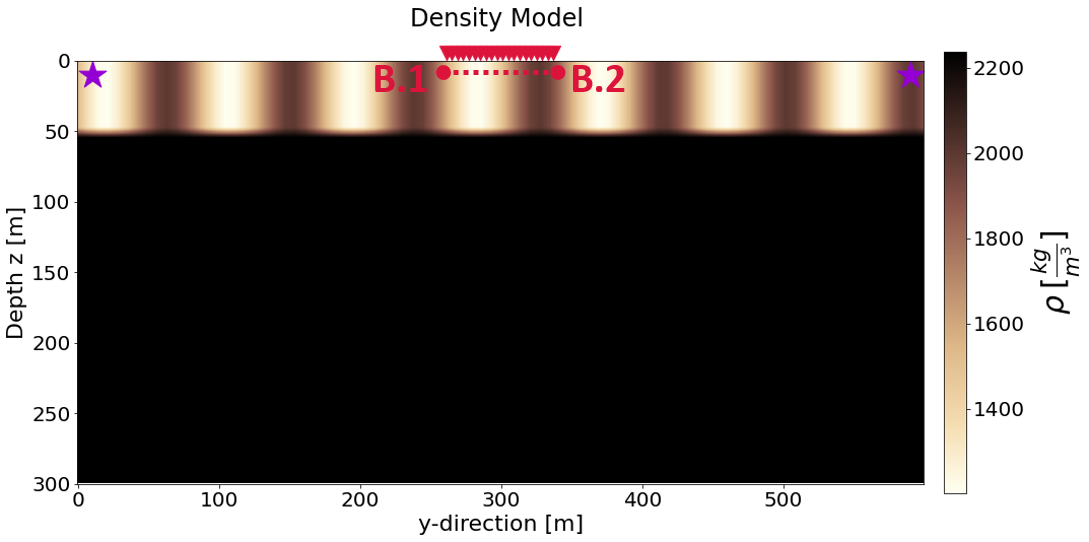
\includegraphics[width =\textwidth, keepaspectratio]{../Figures/rho_model.png}}
	\end{subfigure}
	\hfill{}
	\begin{subfigure}[c]{5.8cm}%{0.37\textwidth}%{5.6cm}
		\centering
		\subfloat[]{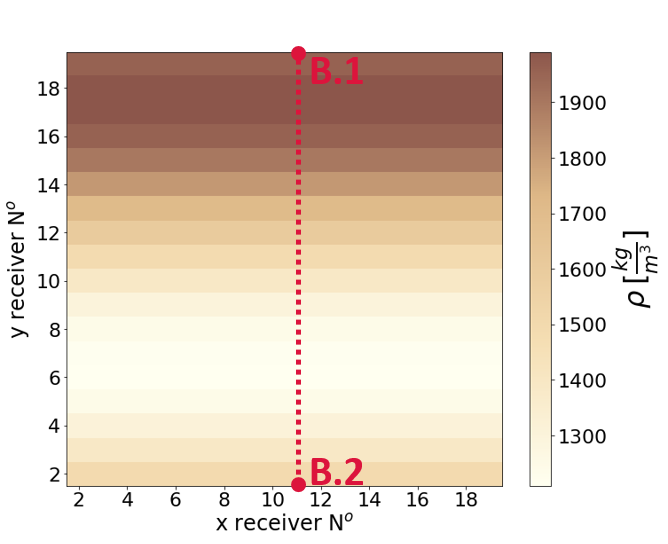
\includegraphics[width = 1\textwidth, keepaspectratio]{../Figures/true_rho_recs.png}}
	\end{subfigure}
	\end{minipage}\\
	%\end{tabular}
	\caption{(a) Acoustic velocity model cross-section in xz-plane. Source locations relative to the receiver array are indicated by stars. Receiver groups marked by red triangles highlight the location of one line of 40 receivers at the surface and their corresponding buried receiver positioned at 1 m depth below. The total array spans an area of 78 $\times$ 78 $m^{2}$ spaced at 2 m intervals across the range [261, 339] m in both x and y directions. For gradiometry relying exclusively on the surface array, derivatives are calculated over a decimated receiver grid spaced at 4 m, whereas all surface receivers at 2 m intervals are used to perform volumetric gradiometry. All plan views showing model parameters are represented on the decimated grid at 4 m receiver spacing. (b) 2D xy-plan view map of the section of the true velocity model spanned by the internal receivers of the surface array. Depth boundary from layer 1 to layer 2 does not correspond to a step function change but a linear increase within the model cell that transitions between properties from the shallower layer to the deeper layer. (c) Density model depth cross-section in yz-plane. (d) 2D xy-plan view map of the section of the true density model spanned by the internal receivers of the surface array. For the pressure signals in Figure \ref{fig:rho_signal}, a constant density model of 1600 $kg/m^{3}$ is used instead for the top layer (Fig. \ref{fig:cst_rho}). Elastic runs are performed with the same velocity and density structure and an additional shear-wave velocity field. Acoustic and elastic forward models have slightly different meshing criteria due to their respective minimum model velocities. }
	\label{fig:TrueModel}
	\end{figure} % \mbox{}

	
	Relevant depth slices and plan view maps of the true acoustic P wave velocity and density model are shown in Figure \ref{fig:TrueModel}. The velocity heterogeneity of the top layer follows a sine function in the x-direction at a wavelength of approximately 113 m. The density structure has a wavelength of 88 m and is rotated by 90$^{o}$ respective to the velocity structure in order to clearly decouple influences of each parameter. The rotation of the orientation of density heterogeneities relative to those in velocity should reveal whether the estimated density structure contains artefacts caused by velocity heterogeneity and vice-versa. Layer 1 is 50 m thick and velocities span the range 1550 m/s to 2300 m/s, densities span 1200 $kg/m^{3}$ to 2000 $kg/m^{3}$, while the deeper layer has a homogeneous velocity of 2700 m/s and density of 2240 $kg/m^{3}$. The receiver array spans an area of 78 $\times$ 78 $m^{2}$ and captures at least half a wavelength of the heterogeneity in both velocity and density structures (Figs \ref{fig:TrueModel}b and \ref{fig:TrueModel}d). Elastic models are constructed analogously to Fig. \ref{fig:TrueModel} with an additional S wave velocity model related to P wave velocity by a Poisson ratio of 0.25. \\


	To test the performance of WEI for simulated ambient noise, five isotropic sources are placed on a circle around the receiver array at a radius of 290 m from the midpoint. They fire Ricker wavelet signatures with different central frequencies ranging from 4.5 Hz to 16 Hz at random time intervals but with the same amplitude to examine whether WEI is robust against waves of overlapping frequency. The sources fire close to the surface at 10 m depth to ensure that the dominant wave energy travels along the surface, allowing the assumption that the pressure gradient in z-direction is small compared to horizontal directions. The increasing velocity with depth in the model ensures that the waves are dispersive as in the true Earth's subsurface.\\
	\DIFaddbegin 

	
	\DIFadd{In addition to the proof-of-concept synthetic model where density structure is orthogonal to the velocity structure, and which is discussed in the main body of the paper, we examine more realistic models that resemble natural borders between geological units more closely in Appendix \ref{sec:APP_D}. Two true density model whose structure oscillate in parallel with the velocity structure of Figure \ref{fig:TrueModel}(a) and (b) are analysed for the acoustic data case.  In Figure \ref{fig:APP_mod_par1}(a) the density gradients follow the same sine curve as the velocity structure and are directly aligned with the velocity gradients (Figure \ref{fig:APP_mod_par1}b), whereas the density and velocity in Figure \ref{fig:APP_mod_par2}(a) and (b) both also vary in the x-direction but are spatially shifted with respect to each other.
}

	
\DIFaddend %	\begin{figure}[H]
%		\centering
%		\captionsetup{width=\linewidth}
%		\includegraphics[width =\textwidth]{TrueMod.png}
%		\caption{(a) Velocity model cross-section in xz-plane. Source locations relative to the receiver array are indicated with the star symbol. Receivers are marked by the red triangles and highlight the location in the model of one line of the 18 internal receiver array spanning an area of 72 $m^{2}$ across the range [264, 336] m in both x $\&$ y directions. (b) 2D xy-plan view map of true velocity model as spanned by surface receiver array. (c) Density model depth cross-section in yz-plane. (d) 2D xy-plan view map of true density model as spanned by surface receiver array. For the pressure signals in Figure (\ref{fig:rho_signal}), a constant density model of XXX $g/cm^{3}$ is used.}
%		\label{fig:TrueModel}
%	\end{figure}

	\section{Density fingerprint} \label{sec:fingerprint}
	\subsection{Free surface arrays}
	\subsubsection*{Sensitivity to relative density gradients in full acoustic wave equation}

	The full acoustic wave equation \eqref{eq:FA} can be written in the form of the Helmholtz wave equation and a source term containing relative density gradients $\nabla \rho(\bm{x})/\rho(\bm{x})$ acting on pressure gradients $\nabla P(\bm{x},t)$:

	\begin{align}\label{eq:FA_relGRAD}
		\shoveright \shoveright \shoveright \shoveright \shoveright \shoveright \shoveright \shoveright %\shoveright 
		\; \nabla^{2} P(\bm{x},t) \: - \: \frac{1}{c_{\omega}(\bm{x})^{2}}  \: \partial_{t}^{2} P(\bm{x},t)  &\: = \: \frac{\nabla \rho(\bm{x})}{\rho(\bm{x})} \cdot \nabla P(\bm{x},t) 
	\end{align}

	Relative density gradients influence pressure gradients whenever a spatial density gradient $\nabla \rho(\bm{x})$, that is, a laterally heterogeneous density structure, exists. Otherwise the term on the right-hand side of equation \eqref{eq:FA_relGRAD} becomes zero.  \\

	To illustrate the role that relative density gradients play in influencing wavefield gradients we conduct a synthetic experiment in which we compare Helmholtz and full acoustic spatial pressure gradients of a signal recorded at a single receiver station in the model shown in Figure \ref{fig:TrueModel} with variable density and velocity (Figs \ref{fig:rho_signal}c and \ref{fig:rho_signal}d) to one recorded in a model with the same velocity structure but where density is laterally homogeneous in the top layer at a fixed value of 1600 $kg/m^{3}$ (Appendix \ref{sec:AppendixB}, Fig. \ref{fig:cst_rho}) corresponding to the mean value of the top layer in the variable density model (Figs \ref{fig:rho_signal}a and \ref{fig:rho_signal}b). The spatial pressure gradients are expressed as 
	\begin{equation}\label{eq:spatial_HELM}
	\nabla^{2} P(\bm{x},t)
	\end{equation}
	for the Helmholtz equation \ref{eq:helm} and 
	\begin{equation}\label{eq:spatial_FA}
		\rho(\bm{x}) \: \nabla \cdot \bigg(\frac{1}{\rho(\bm{x})} \nabla P(\bm{x},t) \bigg)
	\end{equation}
	for the full acoustic equation \eqref{eq:FA}. For simplicity of notation, we drop the indication of space and time dependencies of density $\rho$ and pressure $P$ hereafter. By comparing these spatial gradients in their discretized forms, we can establish a difference in discretization coefficients acting on pressure P, which subsequently influences the phase velocity estimates (Table \ref{coeffsT}). In the Helmholtz case, classical discretization coefficients for second order derivatives are used, whereas ratios of density from neighbouring receiver stations dominate the discretization coefficients in the full acoustic case (equations \ref{eq:discr_c} to \ref{rho_coeffs}). If the pressure field passes through a homogeneous medium, the coefficients in the full acoustic case reduce to the Helmholtz coefficients since ratios of adjacent density values are equal to 1: the phase velocity estimates are thus identical in this case regardless of which equation is used for WEI. Whenever the densities between neighbouring receiver stations vary, the full acoustic coefficients contain density ratios not equal to 1 and an effect on the phase velocity estimate is expected depending on whether the Helmholtz or the full acoustic wave equation is used as a basis for WEI.\\

	%\captionsetup{width=.7\textwidth}
	\begin{table}[!htb] 
		\centering
		%\hspace*{1.5cm}
		%\begin{subtable}{.4\linewidth}
		%	\begin{tabular}{ r }
		%		\mbox{} \\ 	
		%		Helmholtz: \\  
		%		%\vspace{0.5cm}
		%		Full Acoustic: \Tstrut\\ 
		%	\end{tabular}
		%\end{subtable}%
		%\hspace*{-3.6cm}
		%\begin{subtable}{.7\linewidth}
			\begin{tabular}{ l c c c c c }
				\hline \mbox{} 
				& [j-1] & [i-1] & [i,j] & [i+1] & [j+1] \\ \hline %\hline
				Helmholtz: & 1     & 1     & -4    &    1  &   1   \\ \newline
				Full Acoustic: & $\frac{1}{2}$ $\bm{g}_{[0,-]}'$\Tstrut  &  $\frac{1}{2}$ $\bm{g}_{[-,0]}'$\Tstrut  & $\frac{1}{2}$ $\bm{g}_{[\pm,\pm]}'$\Tstrut   &    $\frac{1}{2}$ $\bm{g}_{[+,0]}'$\Tstrut  &    $\frac{1}{2}$ $\bm{g}_{[0,+]}'$\Tstrut\Bstrut\\  \hline 
			\end{tabular}
		%\end{subtable} 
		\caption{If divided by receiver spacing $\Delta x^{2}$, the presented values correspond to finite difference discretization coefficients on a regular grid (Fig. \ref{fig:gridFD}) for second order spatial pressure gradients in Helmholtz (\ref{eq:helm}) and full acoustic (\ref{eq:FA}) equations respectively. Helmholtz coefficients correspond to the classical central finite difference discretization values. Full acoustic coefficients are dependant on density ratios $\bm{g}'$ of neighbouring receivers.} \label{coeffsT} %Helmholtz and full acoustic discretization coefficients are identical in homogeneous media but vary in laterally heterogeneous media.
	\end{table}
	%We attribute the difference in spatial derivatives to density gradients in the subsurface 
	%Density gradients influence/drive the difference between helmholtz and full acoustic spatial derivatives. Thus, we define their difference as the measurable signal caused by density gradients.
	%The density gradient signal is defined as $\Delta \: \rho$ = $\rho [\nabla \frac{1}{\rho} \nabla P \: - \: \nabla^{2} P]$.

	%\captionsetup{width=\textwidth}

	This behaviour of the spatial gradients becomes obvious in both acoustic (Figs \ref{fig:rho_signal}a and \ref{fig:rho_signal}c) and elastic (Figs \ref{fig:rho_signal}b and \ref{fig:rho_signal}d) media. In the homogeneous model case, Helmholtz and full acoustic spatial gradients are the same, resulting in no difference between Helmholtz and full acoustic spatial gradients (Figs \ref{fig:rho_signal}a and \ref{fig:rho_signal}b). In the model with variable density we observe a clear change in wave amplitude and a phase shift between spatial gradients which is prominent between recording times 1 s and 1.7 s in the acoustic case. After 1.7 s changes in the shape of the waveforms of Helmholtz and full acoustic gradients are observed in the acoustic example (Figure  \ref{fig:rho_signal}c). Density gradients therefore create a clearly distinguishable fingerprint (Figs \ref{fig:rho_signal}c and \ref{fig:rho_signal}d), especially in acoustic media. The difference in Helmholtz and full acoustic spatial gradients is affected less strongly in elastic media even though underlying density gradient values are the same in both acoustic and elastic models. The fingerprint $\bm{\Gamma}$ is defined as the difference between normalised spatial gradients: 
	\begin{equation}\label{eq:fingerprint}
		\bm{\Gamma} = [\rho \nabla \cdot \bigg(\frac{1}{\rho} \nabla P\bigg)] \: - \: [\nabla^{2} P] \; = \; \frac{\nabla \rho}{\rho} \cdot \nabla P 
	\end{equation}
	In the analysed synthetic model, density varies exclusively in the y-direction, where $\partial_{x} \rho =0$ and $\bm{\Gamma}$ reduces to the form:
	\begin{equation}
		\bm{\Gamma} =  \; \frac{1}{\rho} \: \partial_{y} \rho \: \partial_{y} P
	\end{equation}
	Neglecting information on density structure results in Helmholtz gradients that are not representative of the propagation medium. This causes the phase velocity to be either over- or underestimated by WEI when using the Helmholtz equation in a variable density medium. 

		\begin{figure}[H] \centering
		%\begin{tabular}[c]{c c}
			\begin{subfigure}[t]{0.49\linewidth}
				\centering
				\subfloat[]{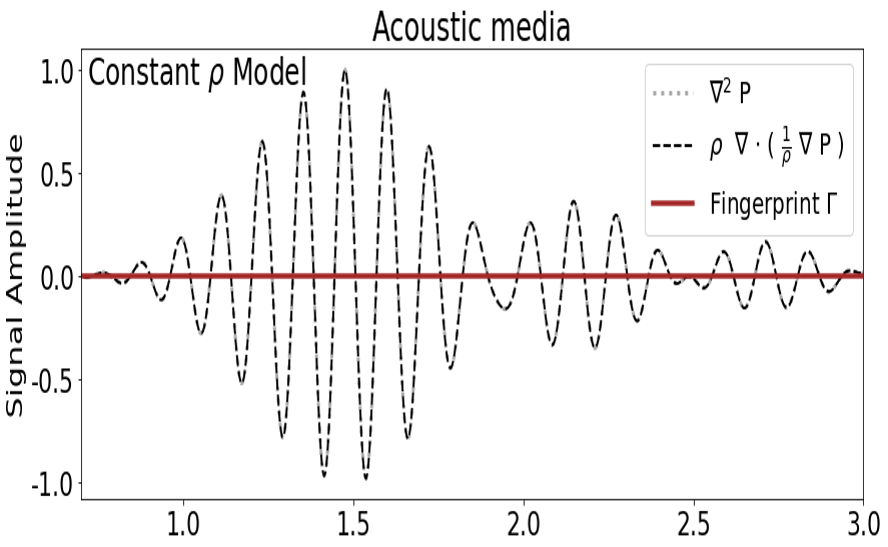
\includegraphics[width =\textwidth, keepaspectratio]{../Figures/rho_signal_spatial_1.png}}
			\end{subfigure}\hspace{0.1cm}
			\begin{subfigure}[t]{0.49\linewidth}
			\centering
			\subfloat[]{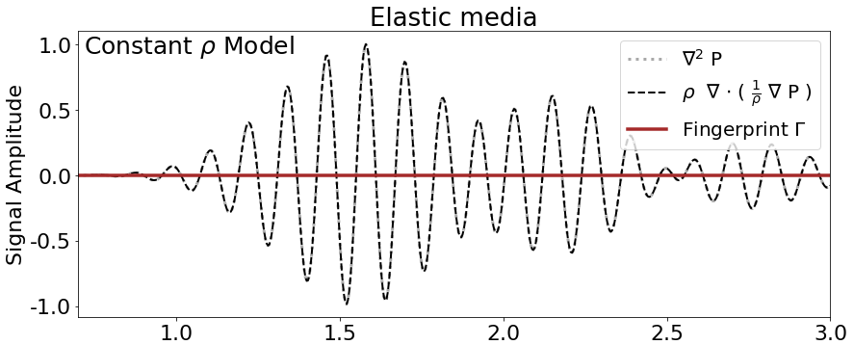
\includegraphics[width =\textwidth, keepaspectratio]{../Figures/ELA_rho_signal_spatial_1.png}}
			\end{subfigure}\\
			\begin{subfigure}[c]{0.49\linewidth}
				\centering
				\subfloat[]{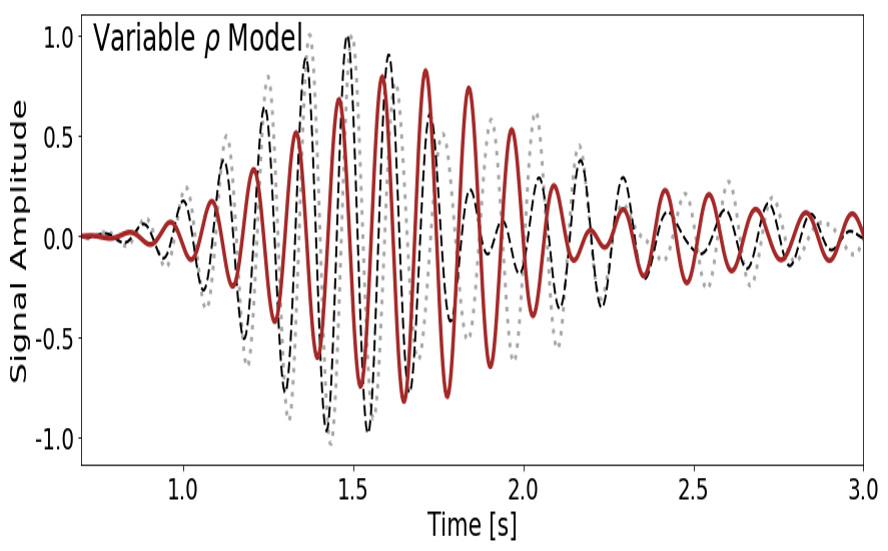
\includegraphics[width = \textwidth, keepaspectratio]{../Figures/rho_signal_spatial_2.png}}
			\end{subfigure}\hspace{0.1cm}
			\begin{subfigure}[c]{0.49\linewidth}
				\centering
				\subfloat[]{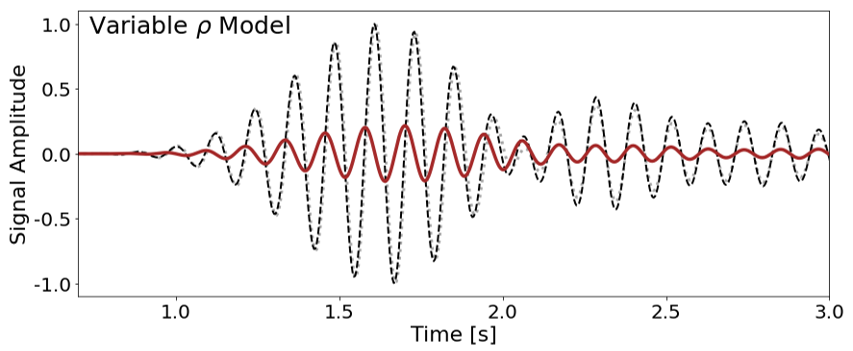
\includegraphics[width = \textwidth, keepaspectratio]{../Figures/ELA_rho_signal_spatial_2.png}}
			\end{subfigure}
		\caption{Effect of density gradients in 3D acoustic (a and c) and elastic media (b and d). Panel (a) and (b) show the discretized Helmholtz (dotted grey) and full acoustic (dashed black line) normalised spatial gradients at receiver [13,13] for a constant acoustic and elastic density model (Appendix \ref{sec:AppendixB}, Fig. \ref{fig:cst_rho}) respectively. The difference between Helmholtz and full acoustic gradients (solid red line) shows that constant density has no influence on the measured wavefield. Panel (b) and (d) show the same information for a heterogeneous density model (Fig. \ref{fig:TrueModel}c and\ref{fig:TrueModel}d) in acoustic and elastic media respectively. The difference between Helmholtz and full acoustic gradients contains the signal generated by the density gradient in y-direction. The influence of the density gradient can clearly be distinguished (solid red line). In this example, the wavefield is filtered between 7 Hz to 9 Hz.}% Panel (c) shows the temporal gradients from the constant density model (dashed grey) and the variable density model (dotted blue) with their density effect (solid black).}
		\label{fig:rho_signal}
		\end{figure}%\mbox{}

	%In elastic media, density is know to be influencing the amplitude of the wavefield \cite{operto_miniussi}.

%	\begin{figure}[H]
%		\centering
%		\captionsetup{width=\linewidth}
%		\includegraphics[width =0.7\textwidth]{rho_signal_spatial.png}
%		\caption{Effect of density in 3D acoustic media. Panel (a) shows the discretized Helmholtz (dashed grey) and Full Acoustic (dotted blue line) spatial gradients for a constant density model. Constant density has no influence on the measured wavefield. Panel (b) shows the same information for a heterogeneous density model. The influence of the density can clearly be distinguished (solid black line).}% Panel (c) shows the temporal gradients from the constant density model (dashed grey) and the variable density model (dotted blue) with their density effect (solid black).}
%		\label{fig:rho_signal}
%	\end{figure}

	%Also the temporal gradients show the direct impact on the wavefield ...
	%\begin{figure}[H]
	%	\centering
	%	\captionsetup{width=\linewidth}
	%	\includegraphics[width =0.6\textwidth]{rho_signal_temp.png}
	%	\caption{Shows temporal gradients from the constant density model (dashed grey) and the variable density model (dotted blue) with their density effect (solid black).}
	%	\label{fig:rho_signalTEMP}
	%\end{figure}
	%\newpage
	\subsection{Volumetric arrays}
	\subsubsection*{Sensitivity to density in free surface fully elastic wave equation}

	The linear equation derived from the vertical component of the Lax-Wendroff corrected full elastic wave equation puts constraints on density directly. Equation \eqref{eq:FS_RHO_linREG} shows that density linearly relates the temporal and spatial derivatives of displacement to the pressure term. In Fig. \ref{fig:signal_rho_ELASTIC} it becomes clear that the left- and right-hand sides of eq. \eqref{eq:FS_RHO_linREG} are related by a scaling factor. By fitting a regression line with the slope of the inverse of true density in the heterogeneous forward model, a coefficient of determination $R^{2}$ close to 1 is obtained suggesting that the scaling factor between left- and right-hand sides corresponds to the density of the medium. Fig. \ref{fig:signal_rho_ELASTIC}(b) shows that residuals are essentially zero between left-hand and right hand sides of eq. \eqref{eq:FS_RHO_linREG} if the true density is substituted. The density signal behaves analogously in homogeneous media.

	\begin{figure}[H] \centering
		%\begin{tabular}[c]{c c}
		\begin{subfigure}[t]{0.8\linewidth}
			\centering
			\subfloat[]{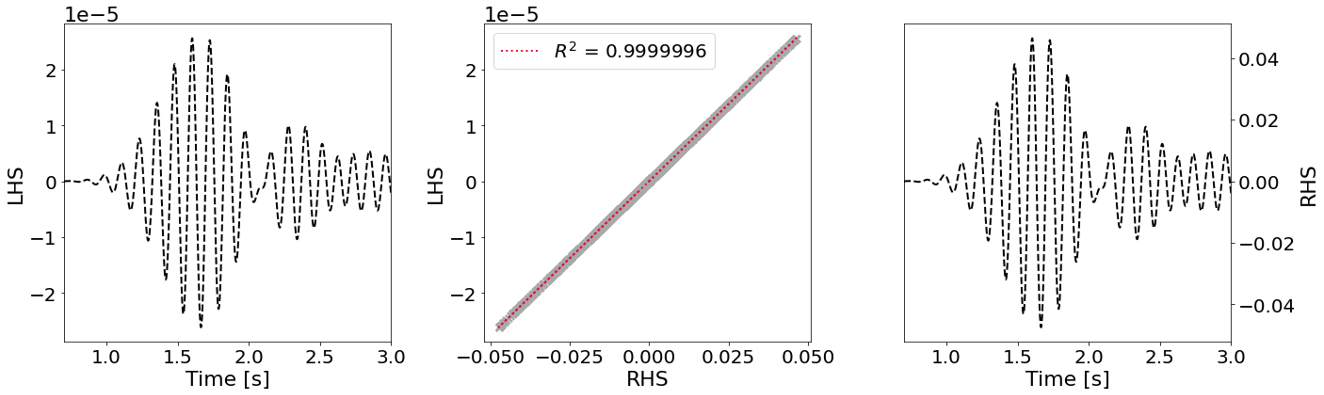
\includegraphics[width =\textwidth, keepaspectratio]{../Figures/rho_signal_elastic1.png}}
		\end{subfigure}\\
		\begin{subfigure}[t]{0.8\linewidth}
			\centering
			\subfloat[]{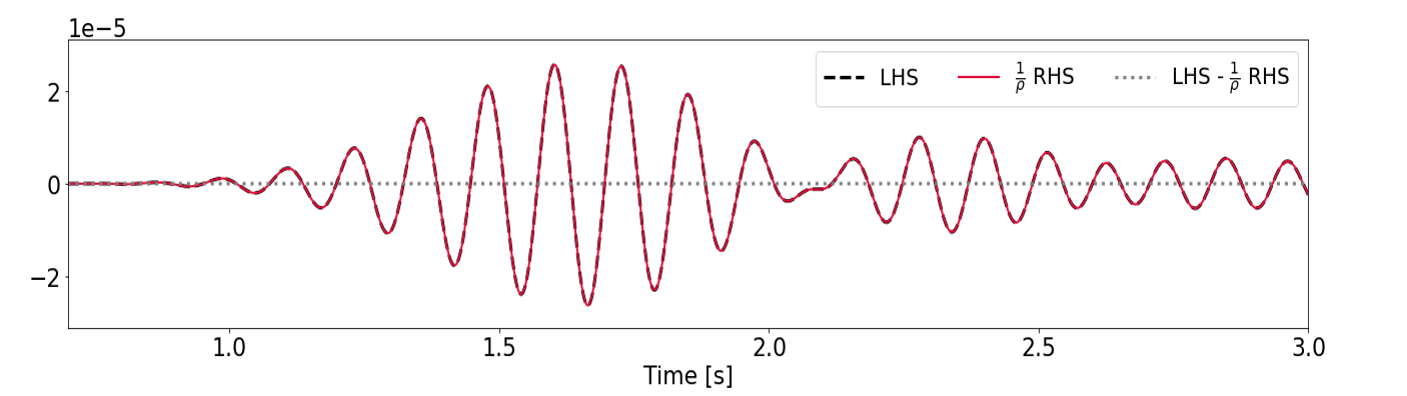
\includegraphics[width =\textwidth, keepaspectratio]{../Figures/rho_signal_elastic2.png}}
		\end{subfigure}
	\caption{Role of density at the free surface of 3D elastic media (\DIFdelbeginFL \DIFdelFL{heterogenous }\DIFdelendFL \DIFaddbeginFL \DIFaddFL{heterogeneous }\DIFaddendFL forward model (Fig. \ref{fig:TrueModel})) shown at the example receiver at location [13,13]. The wavefield is filtered around a central frequency of 8 Hz with a bandpass of 2 Hz. Panel (a) shows the waveform of the discretised left-hand side (left column) and right-hand side (right column) of eq. \eqref{eq:FS_RHO_linREG} when true velocity model parameters are used. The middle column in (a) shows a scatter plot of left- and right- hand data with a regression line of a slope corresponding to the inverse of true density at receiver [13,13]. $R^{2}$ is the coefficient of determination defining the goodness of fit of the regression line and the data. Panel (b) shows the residuals (LHS - 1/$\rho$ RHS) between left- and right-hand side of equation \eqref{eq:FS_RHO_linREG} if the true model density is used.}
	\label{fig:signal_rho_ELASTIC}	
	\end{figure}


	\section{Inversion Results}
	We now present results from the iterative inversion process for density and phase velocity using simulated ambient noise. In section \ref{sec:rho_est} we investigate the performance of density estimation in acoustic media at a central frequency of 8 Hz where the wavefield data is filtered with a narrow bandpass in the range 7 Hz to 9 Hz. We then show how the obtained density information affects the accuracy of phase velocity estimates based on WEI of the full acoustic wave equation, and how random noise impacts the robustness of these estimates. We then investigate the quality of density inversion over a broader frequency range from 4 Hz to 14 Hz and the impact that full WEI has on estimates of phase velocity dispersion curves. In section (\ref{sec:elasticRES}) we discuss the estimated density results in elastic media for a wavefield filtered around 8 Hz obtained with the same iterative inversion workflow. Misfit functions are presented to illustrate trade-offs between density and phase velocity in both acoustic and elastic media (Section \ref{sec:sensitivities}). We then show the density results in elastic media, obtained by gradiometric linear regression from the full elastic wave equation at the free surface (Section \ref{sec:vol_res}).\DIFaddbegin \\
	\DIFaddend 

	\DIFaddbegin \DIFadd{An outline of the structure of the result section summarising the analysed data types, array configurations and equation at the basis of the inversion methods, is given in Table \ref{struct}.
	}

	\begin{table}[!htb]
		\centering
		\begin{tabular}{l l l}
			\hline
			\textbf{\DIFaddFL{Array Type}} \DIFaddFL{\hspace{0.2cm} }& \textbf{\DIFaddFL{Data medium}} & \textbf{\DIFaddFL{Equation for WEI}} \\ 
			\hline 
        	\multirow{2}{*}{\makecell[l]{Free Surface\\ (Section \ref{sec:FSArr})}} & \DIFaddFL{- Acoustic (Section \ref{sec:rho_est}) }& \multirow{2}{*}{\makecell[l]{Full Acoustic (From Section \ref{methS}, Eq. \ref{eq:FA})} } \\ %DIF > \vspace{0.1cm}
			& \DIFaddFL{- Elastic (Section \ref{sec:elasticRES}) }& \\ \noalign{\vskip 0.6ex} \hdashline \noalign{\vskip 0.6ex}
%DIF > 			\hdashline
			\makecell[l]{Volumetric \\(Section \ref{sec:vol_res})} & \DIFaddFL{- Elastic (Section \ref{sec:vol_res_el}) }& \makecell[l]{Modified Full Elastic Free Surface \\ (From Section \ref{methV}, Eq. \ref{eq:freeSurf_P2})} \\ 
			\hline
		\end{tabular} %DIF >  \hspace{4.4pt}
		\caption{\DIFaddFL{Overview of the used WEI approaches that structure the result section. For the inversion method based on free surface arrays (Fig. \ref{fig:gridFD}a) and volumetric arrays (Fig. \ref{fig:gridFD}b), used to produce the following results, the reader can refer to Section \ref{methS} and \ref{methV}, respectively. For free surface arrays, the main underlying equation used to obtain density is the full acoustic wave equation \eqref{eq:FA}. Density inversion with surface arrays, based on full acoustic WEI, is tested on both acoustic and elastic synthetic datasets. For volumetric arrays, density is obtained on the basis of a modified version of the full elastic wave equation \eqref{eq:freeSurf_P2} at the free surface in which both vertical particle velocity and pressure appear.}}
		\label{struct}
	\end{table}

	
	\DIFaddend \subsection{Free surface arrays} \DIFaddbegin \label{sec:FSArr}
	\DIFaddend \subsubsection{Acoustic Data} \label{sec:rho_est}
	\subsubsection*{Density Estimation} 

	Figure \ref{fig:rho_est_8Hz}(a) shows the density inversion results as a mean over all cross sections in x (Fig. \ref{fig:rho_est_8Hz}a, left) and y direction (Fig. \ref{fig:rho_est_8Hz}a, right). Corresponding lateral relative y- and x-gradients in density are depicted in Figure \ref{fig:rho_est_8Hz}(b) in the left and right column respectively. Without damping, there is no constraint on the absolute value of the density.  Hence, the inversion process is quite sensitive to different initial damping parameters $\Theta_{d}$. As a rule of thumb, setting the initial damping parameter at 10$\%$ of the mean amplitude of all recorded pressure signals stabilized our inversions. The mean value over the true density model is fed to the inversion as the initial homogeneous guess $\rho_{init}$. \\

	We clearly see the effect of the damping term in the first iteration where the inverted density estimate is skewed towards the initial guess. After the initial iteration we decrease the damping parameter by a factor of 10 and keep it constant for a total of 100 iterations. Lowering the damping parameter gives less weight to the prior information. Tests showed that the inversion process is only sensitive to the initial damping parameter: decreasing the damping parameter further after the initial stabilization phase did not have an effect on the final result, but it allowed the inversion to converge faster towards a minimum misfit solution. After only 10 iterations of alternately updating velocity and density, the density estimates approximate the true solution fairly well and remain stable over subsequent iteration steps until the end of the inversion process is reached. The initial spiky character observed in x-direction might arise since we did not impose any smoothness constraints on the inversion. The logarithm of the data misfit vector $\bm{\delta_{d}}$ of dimension [R$\times$1]
	\begin{equation}\label{eq:datamisfit}
		\bm{\delta_{d}} \: = \: \frac{\Sigma_{n=1}^{n_{t}} \big( \bm{J}'_{n} \: \bm{m}' - \bm{d}_{n} \big)^{2}}{n_{t}}
	\end{equation}
	for the predicted model at each iteration is shown in Figure \ref{fig:rho_est_8Hz}(c) and is used to determine whether the iteration delivers satisfactory results. At the initial iteration the logarithm of the full acoustic misfit of -7.0 is comparable to the Helmholtz misfit level at a value of -6.1. From there, the data misfit continually decreases with progressing iteration steps. In the first 10 iterations, the logarithmic misfit decreases rapidly from -7.0 to -13.2 at iteration 10. This steep drop correlates well with the improvement on the relative parameter error on the relative density gradient in y-direction. The relative error of parameter p at each location i,j is defined as the difference between the absolute values of true and estimated values $|p|^{true}$ and $|p|^{estimate}$ divided by the true values
	\DIFdelbegin %DIFDELCMD < 

%DIFDELCMD < 	%%%
\DIFdelend \begin{equation} \label{eq:error}
		|Error|_{i,j} = 100|\frac{|p|^{true}_{i,j} - |p|^{estimate}_{i,j}}{|p|^{true}_{i,j}}|
	\end{equation}
	\DIFdelbegin %DIFDELCMD < 

%DIFDELCMD < 	%%%
\DIFdelend where, in this instance, parameter p stands for the relative x- or y-density gradients  $\partial_{x} \rho/\rho$ and $\partial_{y} \rho/\rho$ respectively but can stand for any other estimated quantity. \DIFaddbegin \DIFadd{In the case where the true value in equation \eqref{eq:error} is equal to 0, the denominator is scaled by 1.  }\DIFaddend After 12 iterations the logarithm of the misfit remains almost constant around a value of -13.5 and only improves marginally to -13.9 until the inversion is stopped at iteration 100. The density gradient result with minimum parameter error to the true model in x-direction is achieved at iteration step 21. \\

	The slight increase in parameter error on density thereafter is likely to originate from the velocity updates dominating the misfit evolution. Velocity has a much stronger effect than the density since it appears squared in the full acoustic wave equation. We showed in Figure \ref{fig:rho_signal} that in a medium with homogeneous density the spatial gradient expressions from the Helmholtz and the full acoustic equation are identical and so phase velocity estimates remain unaffected by homogeneous densities across the array. Since density is constant in the x-direction, the true phase velocity is only dependent on density structure in the y-direction. Given the poor constraints on density in the x-direction the mean estimate on the density gradient in x-direction deviates, if only slightly ($\pm$ 0.15$\%$), from the true value of zero (Fig. \ref{fig:rho_est_8Hz}b). This introduces artefacts in the phase velocity estimates which in turn influence density estimates negatively throughout the iterative process. Nevertheless, in our experiments the data misfit minimum does tend to indicate when parameter estimates are reasonably accurate. Cross-talk between density and velocity appears to be weak as density
\DIFdelbegin \DIFdel{structure of the true model could be reconstructed successfully with reasonable accuracy without major artefacts (Fig. \ref{fig:rho_est_8Hz}).
}\DIFdelend 

	\begin{figure}[H] \vspace{-1.5cm} \centering
		\begin{tabular}[c]{c}%{c}
		\begin{subfigure}[c]{0.72\linewidth}
			\centering
			\subfloat[]{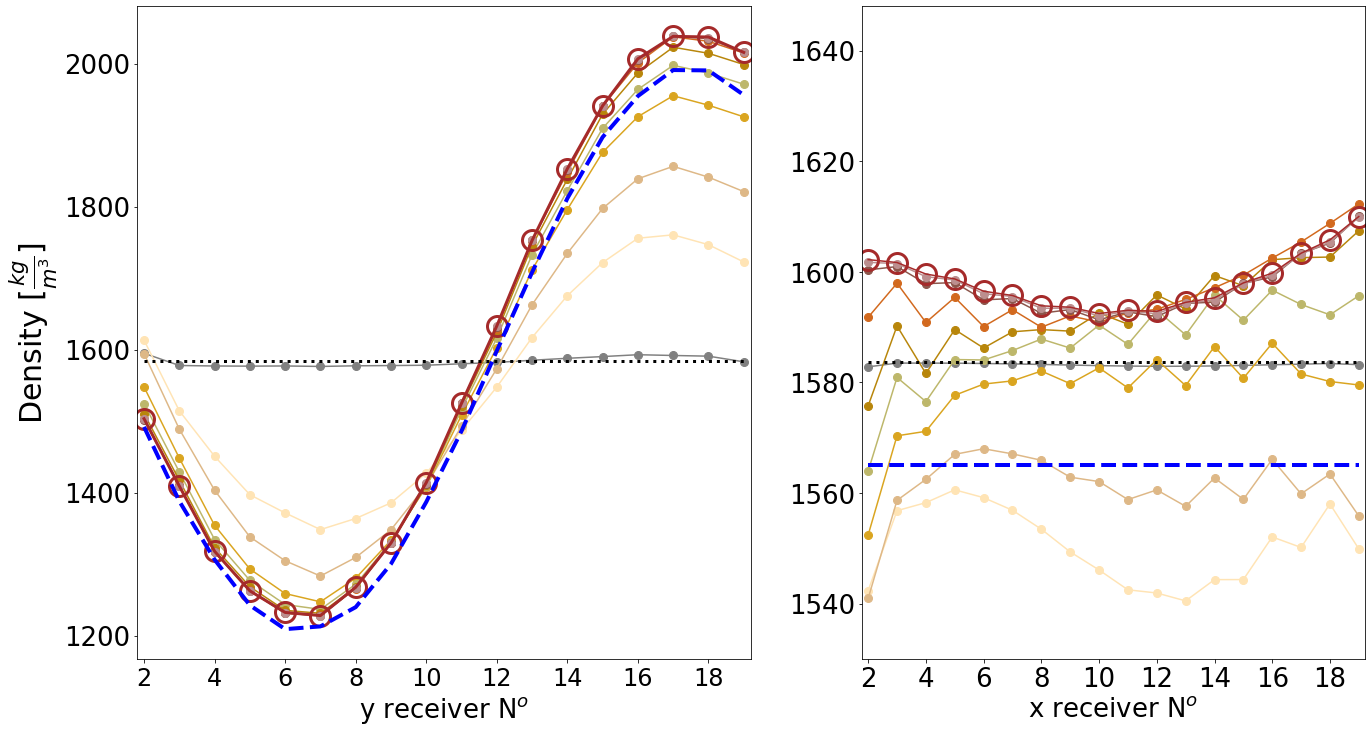
\includegraphics[width =\textwidth]{../Figures/download.png}}%{rho_iterations_8Hz.png}}
		\end{subfigure}\\ 
		\begin{subfigure}[c]{0.718\linewidth}%{0.8\linewidth}
			\centering
			\subfloat[]{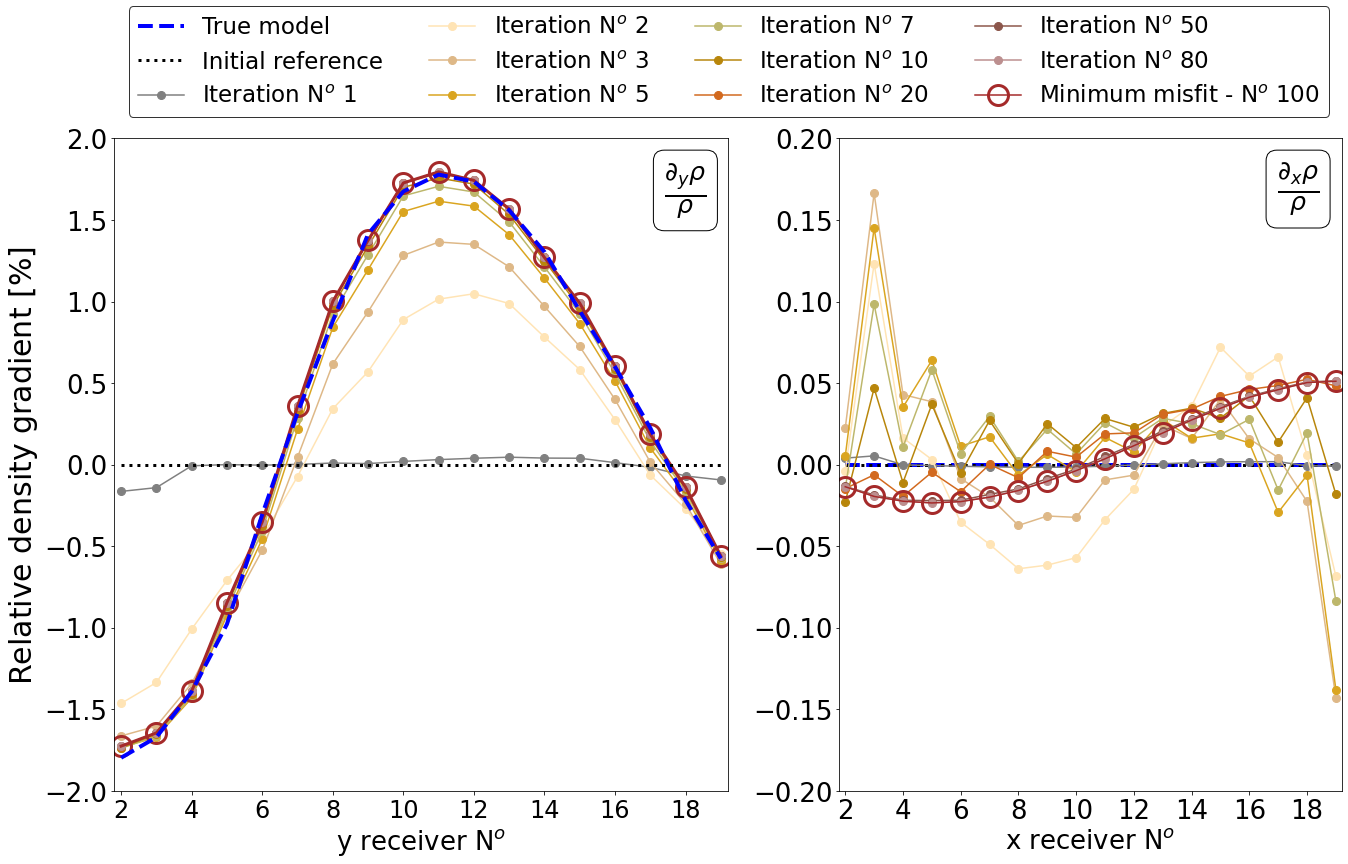
\includegraphics[width = \textwidth]{../Figures/download_gradient_REL.png}}%{iterations_min.png}}
		\end{subfigure} \\ 
		\begin{subfigure}[c]{0.7\linewidth}
		\centering
		\subfloat[]{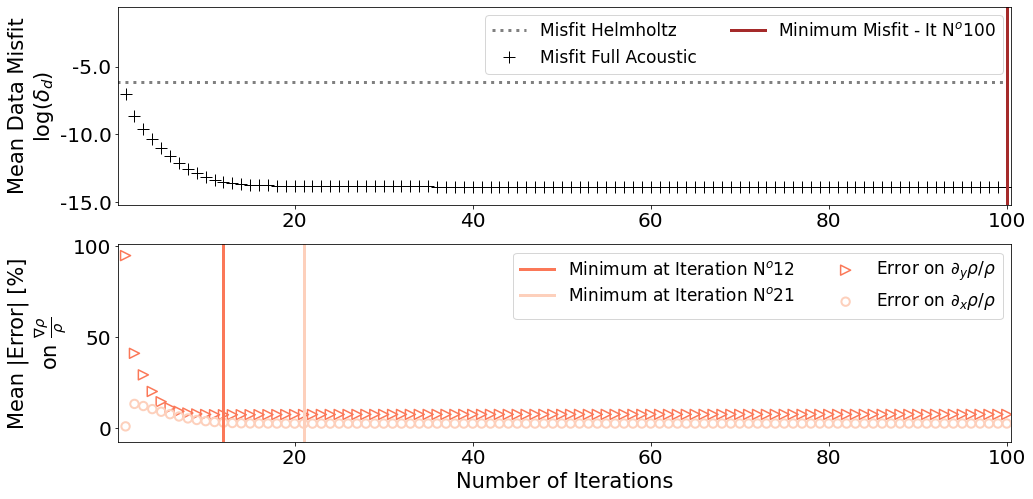
\includegraphics[width = \textwidth]{../Figures/iterations_min_REL.png}}
		\end{subfigure}
		\end{tabular}
	\caption{Inversion result for a wavefield filtered to include frequencies in the range of 7 Hz to 9 Hz. Only the results for the internal receivers 2 to 19 are displayed, as boundary stations need to be disregarded for finite difference estimates. (a) Mean value of inverted density results over all cross-sections in x-plane (left) and y-plane (right) showing the evolution of inverted density results at selected \DIFdelbeginFL \DIFdelFL{points }\DIFdelendFL \DIFaddbeginFL \DIFaddFL{stages }\DIFaddendFL during 100 iterations. True model is depicted as dashed dark blue line and initial model as dotted black line. The minimum misfit result at iteration 100 is highlighted by red circles. (b) Relative density gradients $\nabla \rho/\rho$ of  (a) in y- and x-direction respectively. (c) Logarithm of the mean data misfit evolution over all internal receivers (upper row) and mean parameter error over all internal receivers on x- and y- relative density gradients (lower row) for the full acoustic wave equation (black crosses) over 100 iterations. Their respective minimum value positions are marked by vertical lines in red for minimum misfit at iteration 100, dark orange and light orange at iteration 12 and 21 for minimum parameter error on relative density y- and x-gradients. As a reference, the misfit achieved with linear regression based on the Helmholtz equation is shown by the dotted grey line. The minimum mean parameter error is evaluated only after the initial iteration.}
	\label{fig:rho_est_8Hz}
	\end{figure}

	\DIFaddbegin \DIFadd{structure of the true model could be reconstructed successfully with reasonable accuracy without major artefacts (Fig. \ref{fig:rho_est_8Hz}).}\\

	\DIFadd{Relative density gradient results for models with parallel gradients (e.g., density structure varying in the same direction as the velocity structure) are shown in Appendix \ref{sec:APP_D} (Figure \ref{fig:APP_mod_par1}c and \ref{fig:APP_mod_par2}c) and could also be reconstructed without a significant increase in cross-talk compared to the models with density and velocity gradients orthogonal to each other. Misfits are higher by two to three orders of magnitude but still suggest a good agreement with the data (Figure \ref{fig:APP_mod_par1}d and \ref{fig:APP_mod_par2}d); also the evolution of the mean error on the relative density gradients is comparable to the tested model with orthogonal density and velocity structures.}\\

	\DIFaddend %parameters could be reconstructed successfully to an acceptable degree of accuracy. 
	As discussed in section \ref{sec:fingerprint}, the inversion is predominantly sensitive to the relative changes in density $\nabla \rho/\rho$  where  $\nabla \rho$ corresponds to the gradient of density at a central point $\rho = \rho_{i,j}$ over the finite difference stencil (cf. Fig. \ref{fig:gridFD}), and is less so to the absolute values $\nabla \rho$ (Fig. \ref{fig:damping}). Figure \ref{fig:damping} shows that the minimum misfit estimate of the local density gradient in the y-direction is typically within $\pm 10 \%$ of the true value for relative density changes larger than $ 0.5 \%$ over the width of the spatial finite difference stencil. The accuracy of estimates decreases for very weak relative changes below $ 0.5 \%$. Estimates on absolute values may be biased depending on which initial density guess is fed to the first iteration of the inversion. Results in Figure \ref{fig:rho_est_8Hz}(a) could successfully reconstruct absolute density values due to an appropriate choice of starting model $\rho_{init}$. If the initial guess of bulk density varies more strongly from the true values, the absolute estimates are under- or over-estimated according to the input starting model (Fig. \ref{fig:damping}a, left) because the inversion fits the relative changes in density ratios (Fig. \ref{fig:damping}a, right) as becomes obvious from equation \eqref{eq:FA_relGRAD}. By reconstructing relative density changes, the results are unbiased by the choice of initial density model $\rho_{init}$ (Fig. \ref{fig:damping}a, right). The results of relative density gradients for each local receiver position over the entire grid are shown in Figure \ref{it_min} as 2D plan view maps. 

	
	\begin{figure}[H] \centering 
				\begin{tabular}[c]{c}%{c}
			\begin{subfigure}[c]{0.8\linewidth}
				\centering
				\subfloat[]{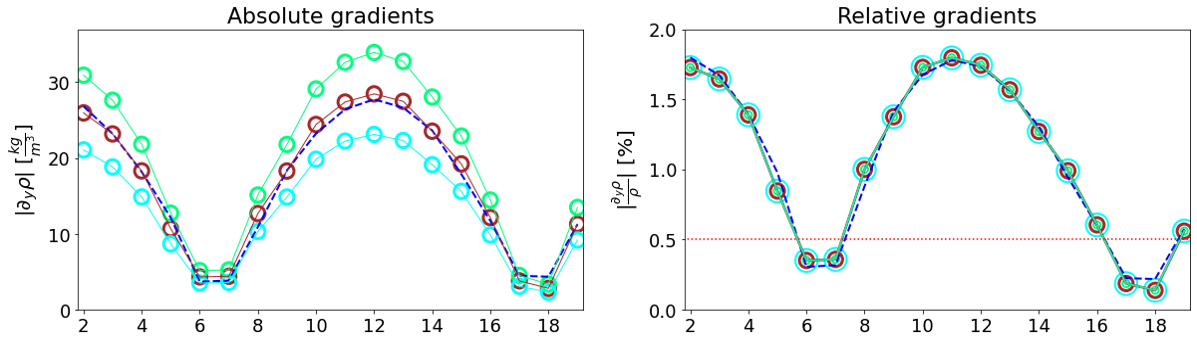
\includegraphics[width =\textwidth]{../Figures/damping_grads.png}}%{rho_iterations_8Hz.png}}
		\end{subfigure}\\ 
		\begin{subfigure}[c]{0.8\linewidth}%{0.8\linewidth}
			\centering
			\subfloat[]{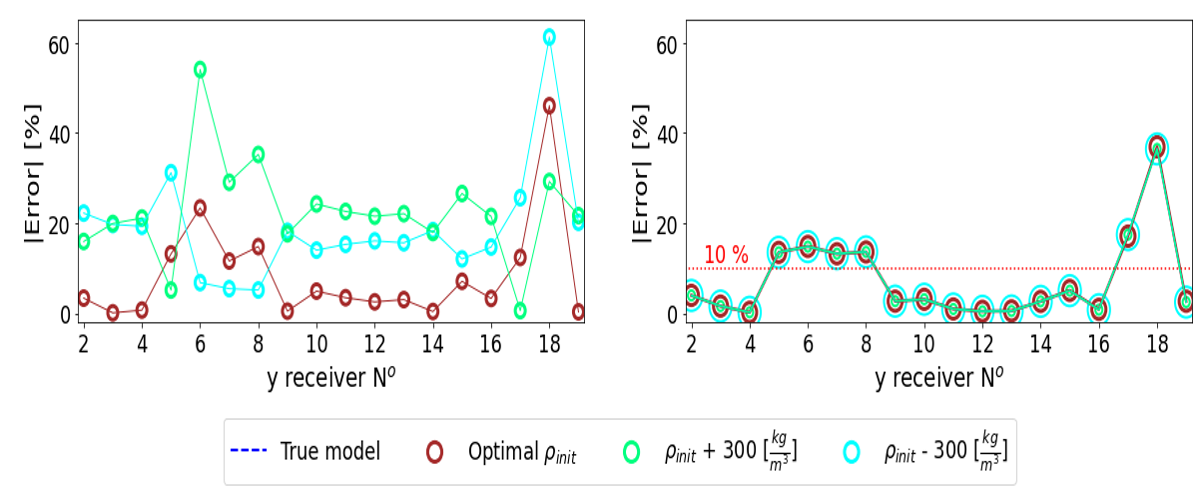
\includegraphics[width = \textwidth]{../Figures/damping_errors.png}}%{iterations_min.png}}
		\end{subfigure} \\ 

		\end{tabular}
		\caption{Impact of initial density guess $\rho_{init}$ on inversion results of (a) absolute density y-gradients $\partial_{y} \rho$ (left) and relative density y-gradients $\partial_{y} \rho/\rho$ (right). Their respective errors (Eq. \ref{eq:error}) are depicted in (b). Results from an optimal $\rho_{init}$ starting model (red circles) correspond to the estimates in Figure \ref{fig:rho_est_8Hz}(a) where $\rho_{init}$ is the mean bulk density of the true model (dashed dark blue line). Results for a less well informed initial guess with higher mean bulk density (green circles) and lower mean bulk density (light blue circles) are shown for comparison.} \label{fig:damping}
	\end{figure}

	\begin{figure}[H]
		\centering
		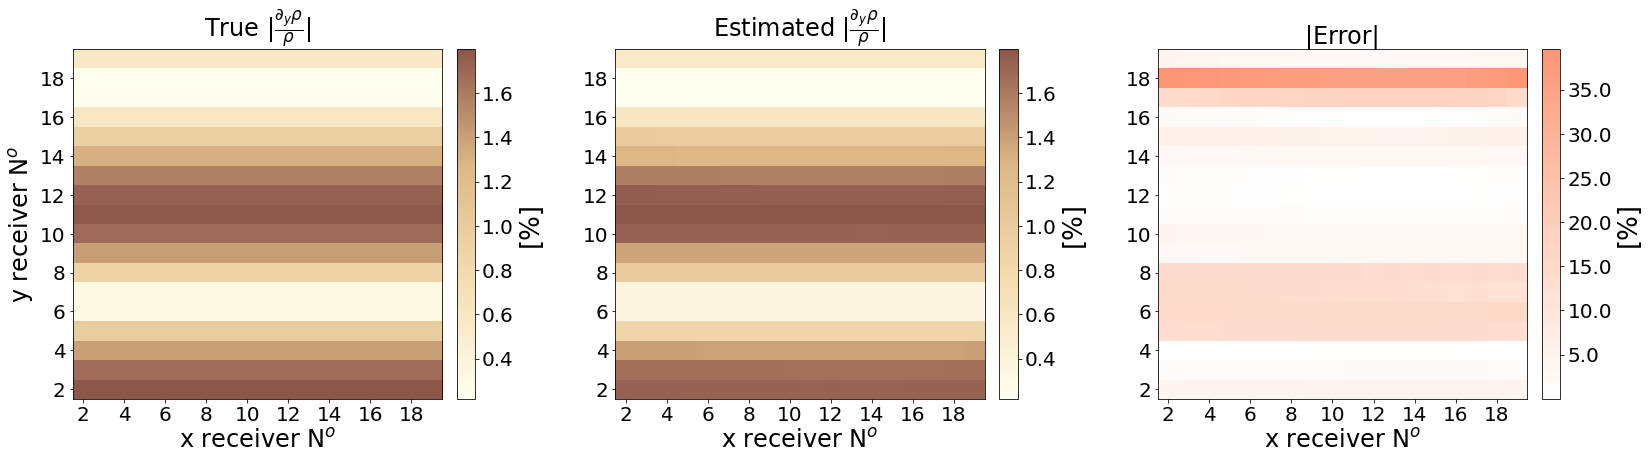
\includegraphics[width = \textwidth]{../Figures/result_min_gradERR_it_REL.png}
		\caption{Plan view of (left) true model and (middle) inversion results for absolute values of relative density gradients in y-direction $\partial_{y} \rho/\rho$ at iteration 100. The corresponding parameter error (Eq. \ref{eq:error}) is shown in the right panel.} \label{it_min}
	\end{figure}
	%To visualize the sensitivities of the inversion towards absolute density values versus density gradients, we analyse the misfit at a fixed central receiver location $[x_{0},y_{0}]$. The density at %the central location is fixed, but both neighbouring cells in y-direction are perturbed in order to investigate the misfit evolution with various gradient options. The density at $[y_{0}+1]$ and %$[y_{0}-1]$ are varying between $\pm$300 $\frac{kg}{m^{3}}$ around the true value at $[x_{0},y_{0}]$ and produce gradient values between $\pm$100 $\frac{kg}{m^{3}}$. For the purpose of %investigating solely the effect of density on the inversion, the phase velocity at the central point is fixed with the value that is obtained from WEI if knowledge on the true density model is %assumed. At the example of receiver [12,12], the misfit function shows a trough-shaped low misfit area that is consistent with the density gradient values of the true model. Accurate estimates on %both the absolute densities at positions $[y_{0}+1]$ and $[y_{0}-1]$ as well as density gradients at $[x_{0},y_{0}]$ are made if the central density is fixed at the true value. If the proposed %density at $[x_{0},y_{0}]$ deviates from the true model value, the estimate on the gradient is still very close to the true one even though the absolute values do not correspond to the true ones. %The misfit is barely influenced by the wrong pair of absolute values at $[y_{0}+1]$ and $[y_{0}-1]$, hence suggesting that multiple absolute density value combinations do explain the data almost %equally well, whereas the misfit varies more strongly with density gradient values. If we change the phase velocity value, we get a faulty estimate on the density gradient.

%	\begin{figure}[H] \centering
%		%\begin{tabular}[c]{c c}
%		\begin{subfigure}[c]{0.3\linewidth}
%			\centering
%			\subfloat[]{\includegraphics[width =\textwidth, keepaspectratio]{misfit_cross.png}}
%		\end{subfigure}
%		\begin{subfigure}[c]{0.8\linewidth}
%			\centering
%			\subfloat[]{\includegraphics[width = \textwidth, keepaspectratio]{F_objective[12,12].png}}
%		\end{subfigure}
%		\caption{(a) }
%		\label{fig:misfit_ANALYSIS_rho}
%	\end{figure}

	
	\subsubsection*{Effect of density gradient on phase velocity estimates} \label{sec:vel_est}
	We now show the extent to which the estimated density structure influences the accuracy of the phase velocity maps. Figure \ref{fig:c_est_8Hz}(a) shows the phase velocity map estimated using the same data as above, but with the Helmholtz wave equation, so without taking density into account in the formulation of wave propagation. Figure \ref{fig:c_est_8Hz}(b) shows phase velocity estimates based on the full acoustic wave equation at iteration 100 where the data misfit is minimal. \\

	By visually comparing these maps to the true velocity structure (Fig. \ref{fig:TrueModel}b) it is obvious that the Helmholtz approach fails to reproduce the relative structure of the subsurface velocity pattern. By contrast, the results obtained by WEI of the full acoustic wave equation yield an improved estimate of the velocity structure that is much closer to the true model in terms of relative structural features. This observation is reflected in the much lower misfit values obtained for the full acoustic model compared to the Helmholtz model (Fig. \ref{fig:c_est_8Hz}c). It is notable how the misfit evolution over the y-axis is dominated by the slope of the density heterogeneity in the true structure (red dashed line). The Helmholtz misfit values approach the full acoustic misfit values at a density gradient close to zero (see green highlight at y-receiver 6 in Fig. \ref{fig:c_est_8Hz}(c)), whereas, for steep changes in density at y-receiver 13 in the model, the Helmholtz equation performs relatively poorly.\\

	Figure \ref{fig:misfit} illustrates the effect of density gradients on phase velocity estimates at two specific receiver stations in the array. Phase velocity squared is given by the slope of the linear relationship between spatial and temporal gradients (Equation (\ref{eq:helm}) for Helmholtz and (\ref{eq:FA}) for full acoustic equation). Figure \ref{fig:misfit}(a) shows that the full acoustic spatial gradients reveal a clearer linear relationship than the Helmholtz model as indicated by a coefficient of determination $R^{2}$ closer to 1. The difference in best fit slope estimates shows that phase velocity is considerably underestimated for the Helmholtz model at receiver [13,13] due to the fact that the relative density structure is neglected in the computation of the spatial gradients. This disparity in the accuracy of phase velocity estimates becomes evident also in the comparison of left-hand and right-hand side signals of the full acoustic and Helmholtz equation (Fig. \ref{fig:misfit}b) and their respective residuals (Fig. \ref{fig:misfit}c). They illustrate that the full acoustic expression matches the pure data vector well, whereas the Helmholtz expression exhibits larger residuals than the full acoustic case for both receiver stations. Incorporating density in the spatial gradient terms of WEI is thus shown to be important in order to estimate phase velocities accurately. 

	\begin{figure}[H] \centering
		%\begin{tabular}[c]{c c}
			\begin{minipage}{\textwidth}
			\begin{subfigure}[c]{0.46\textwidth}
				\flushright
				\subfloat[]{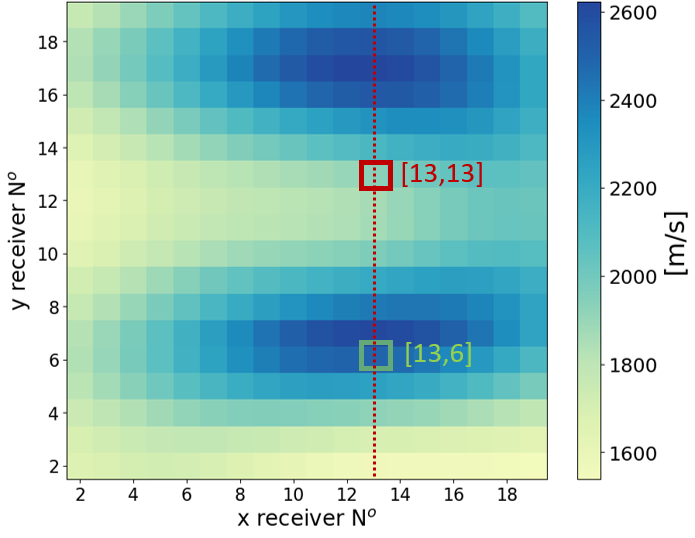
\includegraphics[width =0.9\textwidth]{../Figures/c_helm.png}}
			\end{subfigure}
			\hfill{}
			\begin{subfigure}[c]{0.46\textwidth}
				\flushleft
				\subfloat[]{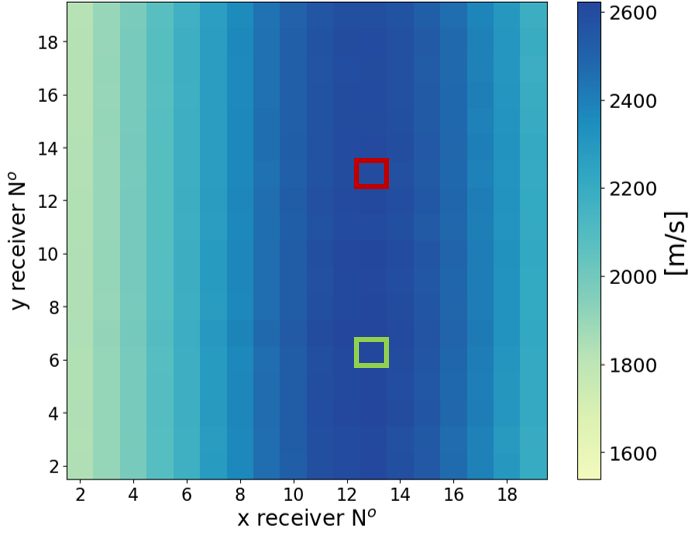
\includegraphics[width = 0.9\textwidth]{../Figures/c_FA.png}}
			\end{subfigure}
			\end{minipage}\\
			\begin{subfigure}[c]{0.81\textwidth}
			\centering
			\subfloat[]{\includegraphics[width = 0.9\textwidth]{../Figures/rho_grad_effect.png}}
			\end{subfigure}
		%\end{tabular}
		\caption{Phase velocity map estimated using (a) linear regression based on Helmholtz wave equation and (b) full acoustic wave equation inversion. Red and green squares mark receiver stations of interest [13,13] and [13,6]. (c) Data misfit post inversion averaged over all x-cross sections (red dotted line in (a) given at example of fixed receiver position x=13) for both phase velocity maps (a) and (b). Black and grey crosses show the logarithm of misfit $\delta_{d}$ in equation (\ref{eq:datamisfit}) for the Helmholtz equation (grey) and the full acoustic wave equation (black). The red dashed curve shows the absolute value of the y-gradient of the true density heterogeneity $\Delta \rho$. Green and red highlighting at receiver station 6 and 13 represent the respective positions in the 2D plan view map.}
		\label{fig:c_est_8Hz}
	\end{figure}

%	\begin{figure}[H]
%		\centering
%		\includegraphics[width = 0.9\textwidth]{rho_grad_effect.png}
%		\caption{text} \label{rho_grad_effect}
%	\end{figure}

	 
	If we compare the misfit residuals for receiver [13,13] (Fig. \ref{fig:misfit}c, left) and [13,6] (Fig. \ref{fig:misfit}c, right), we can see that the full acoustic residuals are of the same order of magnitude at both stations whereas the Helmholtz residuals are two orders of magnitude larger for receiver [13,13]. Receiver [13,13] is located in an area where density is highly variable between the surrounding stations (26 $kg/m^{3}$ from Fig. \ref{fig:c_est_8Hz}c) which explains why the Helmholtz wave equation is subject to much larger residuals than the full acoustic equation. Receiver [13,6] is in an area with only weak variations in density among neighbouring receivers (4 $kg/m^{3}$ from Fig. \ref{fig:c_est_8Hz}c), so the left-hand sides of both Helmholtz and full acoustic equations agree well with the observed data vector. The accuracy of velocity estimates thus depends on the true density gradient across surrounding receivers when using the Helmholtz equation for WEI.

	\begin{figure}[H] \centering 
	%\begin{tabular}[c]{c c}
	\hspace{0.00cm} \begin{subfigure}[c]{0.76\textwidth}
		\centering
		\subfloat[]{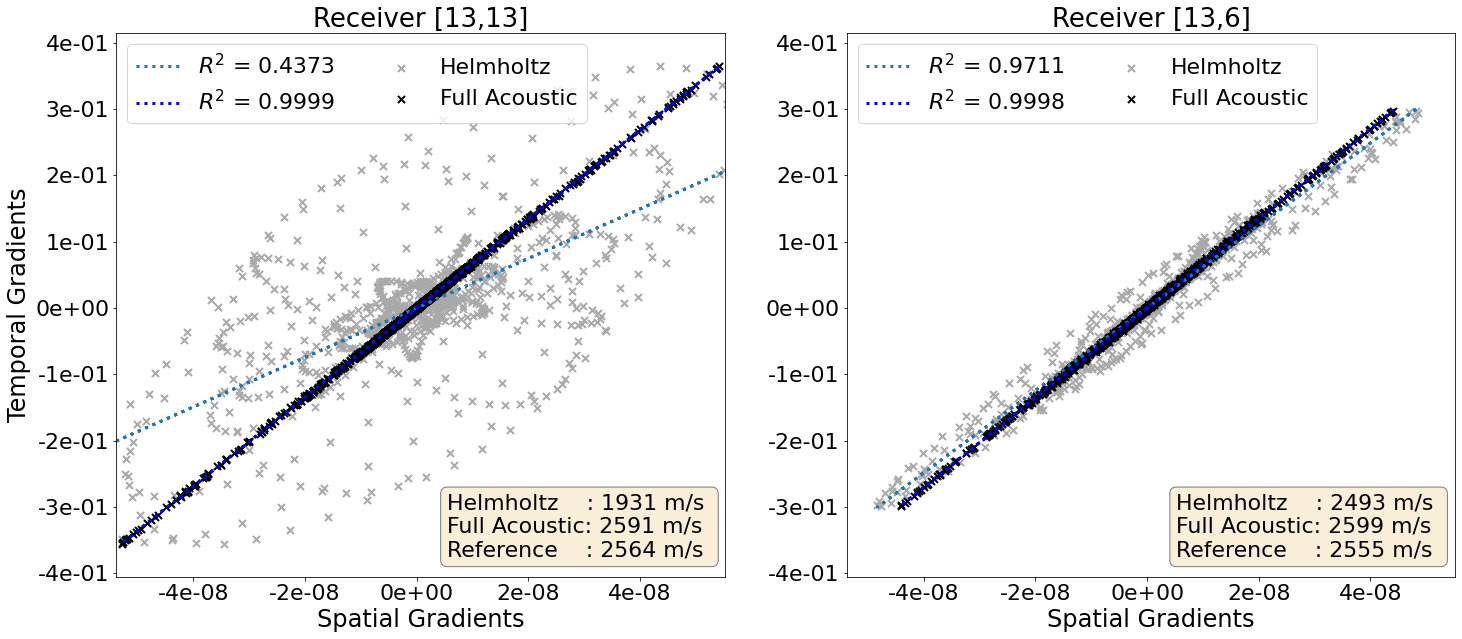
\includegraphics[width =\textwidth, keepaspectratio]{../Figures/scatter_grads.png}}
	\end{subfigure}\\
	\begin{subfigure}[c]{0.76\textwidth}
		\centering
		\subfloat[]{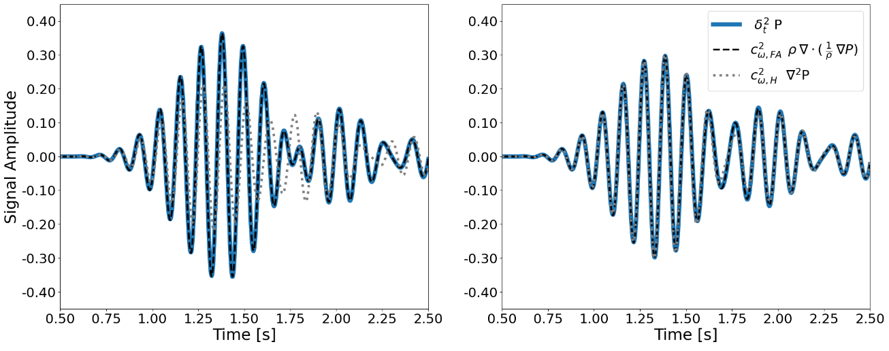
\includegraphics[width = \textwidth, keepaspectratio]{../Figures/residuals1.png}}
	\end{subfigure}
	\begin{subfigure}[c]{0.76\textwidth}
	\centering
	\subfloat[]{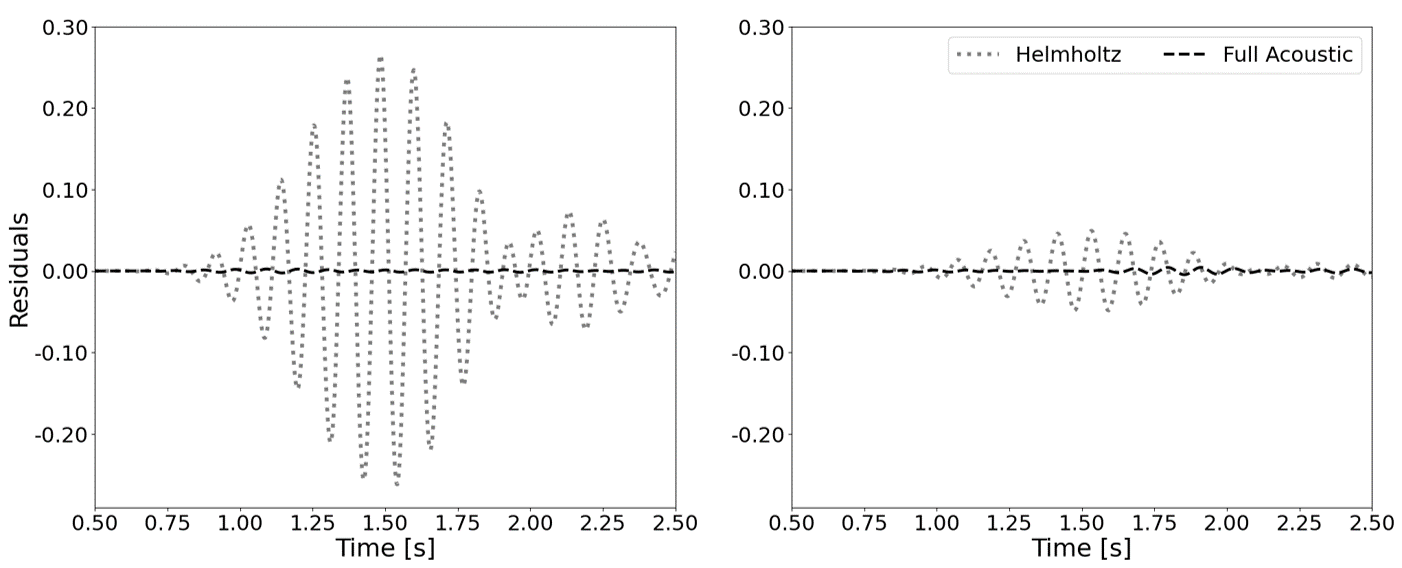
\includegraphics[width = \textwidth, keepaspectratio]{../Figures/residuals2.png}}
	\end{subfigure}
	\caption{(a) Linear relationship between temporal gradients $\delta_{t}^{2}P$ and $\rho \nabla \cdot \big(\frac{1}{\rho} \nabla P\big)$ from \eqref{eq:spatial_FA} for the full acoustic wave equation and $\nabla^{2} P$ from \eqref{eq:spatial_HELM} for the Helmholtz wave equation at the two receiver locations shown in Figure \ref{fig:c_est_8Hz}(a). The coefficient of determination $R^{2}$ denotes the goodness of fit of the data by the linear regression model, and phase velocity estimates using each equation are shown along with the reference velocity obtained for a homogeneous density forward model. (b) Discrete time series of the observed data vector ($\bm{d} = \delta_{t}^{2}P$, solid blue) and the left-hand sides of both Helmholtz ($c_{\omega,H}^{2} \: \nabla^{2} \:P$, black dotted) and full acoustic ($c_{\omega,FA}^{2} \:  \rho \nabla \cdot \big(\frac{1}{\rho} \nabla P\big)$, grey dashed) wave equations respectively, when using the estimated parameter values for phase velocity and density. (c) Respective residuals (difference between right-hand and left-hand side) of both Helmholtz and full acoustic wave equations.}\label{fig:misfit}
	\end{figure} %\mbox{}

	
	\subsubsection*{Changing data frequencies} \label{sec:freqs}

	The effect of the density gradient on phase velocity is persistent over a wider frequency range than was analysed above (Fig. \ref{fig:freq_study}a). In Figs \ref{fig:freq_study}(a) and \ref{fig:freq_study}(b), the dashed blue lines depict the true \DIFdelbegin \DIFdel{constant }\DIFdelend P-wave velocity in y- and x-direction respectively for the shallow layer 1 and the deeper layer 2 of the synthetic model (Fig. \ref{fig:TrueModel}). Due to wave dispersion, the estimated phase velocities should lie in between those two expected absolute thresholds depending on the analysed frequency. The Helmholtz estimates for phase velocity (Fig. \ref{fig:freq_study}a) are consistently underestimated for receivers where density gradients are high (see Fig. \ref{fig:freq_rho} as reference), due to the use in WEI of discretization coefficients that neglect the influence of density (Table \ref{coeffsT}),  whereas they approximate full acoustic (Fig. \ref{fig:freq_study}b) phase velocity estimates at low density gradient values. However, the influence of the density gradients on the Helmholtz phase velocity estimates seems to become smaller with increasing frequency.

	\begin{figure}[H] \centering 
		%\begin{tabular}[c]{c c}
		\begin{minipage}{0.75\textwidth}
			\begin{subfigure}[c]{\textwidth}
				\centering
				\subfloat[]{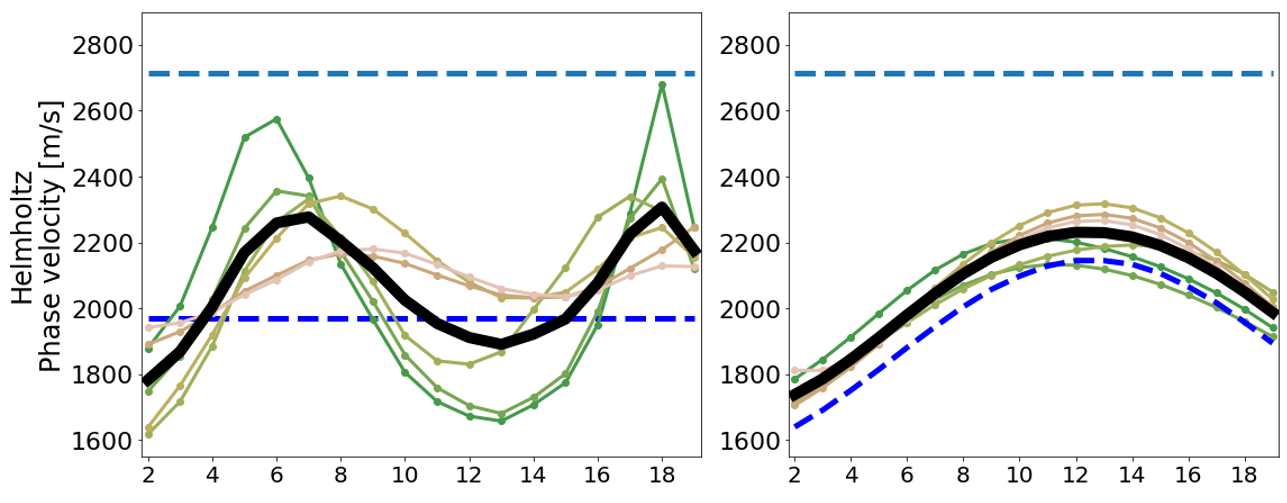
\includegraphics[width =\textwidth, keepaspectratio]{../Figures/freq_study_VEL1.png}}
			\end{subfigure}\\
			\begin{subfigure}[c]{\textwidth}
				\centering
				\subfloat[]{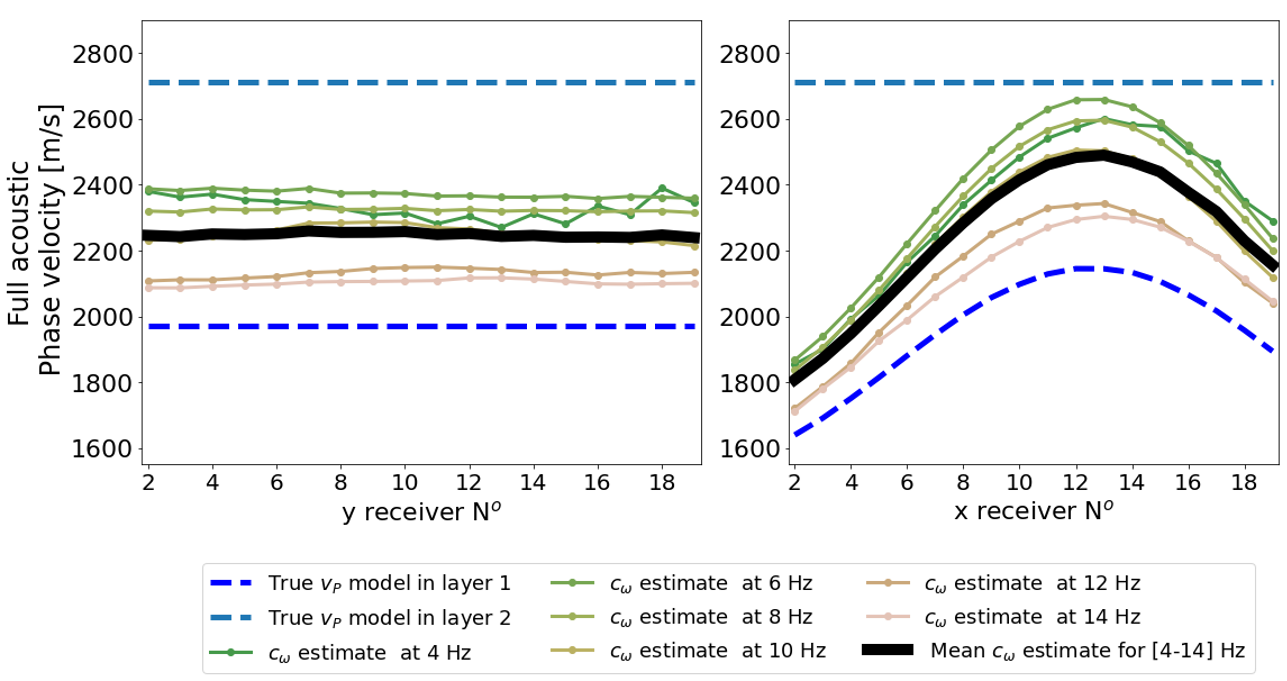
\includegraphics[width = \textwidth, keepaspectratio]{../Figures/freq_study_VEL2.png}}
			\end{subfigure}
		\end{minipage}
		\begin{minipage}{0.2\textwidth}
			\begin{subfigure}[c]{\textwidth}
				\centering
				\subfloat[]{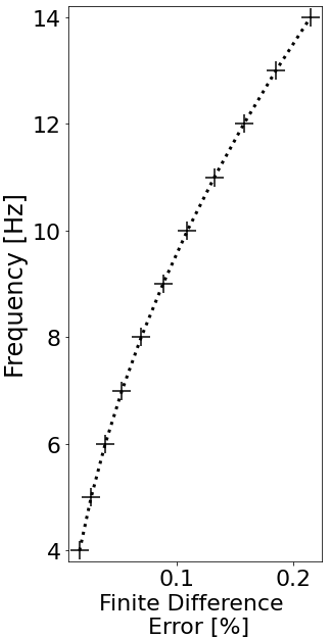
\includegraphics[width = \textwidth, keepaspectratio]{../Figures/Fd_erro.png}}
			\end{subfigure}
		\end{minipage}
		\caption{Results for the estimated phase velocities for 2 Hz wide bandpasses around central frequencies 4 Hz, 6 Hz, 8 Hz, 10 Hz, 12 Hz and 14 Hz from Helmholtz linear regression (a) and full acoustic WEI (b). For the estimation of full acoustic phase velocities, density information as shown in Figure \ref{fig:freq_rho} is used. The mean value over all the frequency results is shown for both full acoustic and Helmholtz velocities in a black solid line. (c) shows the error evolution over frequency for the $2^{nd}$ order accurate approximation of the spatial gradients with a spacing of 4 m used in this example (see Appendix \ref{sec:Appendix}).}
		\label{fig:freq_study}
	\end{figure}
	%Suggesting less sensitivity to density at higher frequencies and phase velocities are less corrupted? sth to do with scale of heterogeneity compared to min wavelength?

	
	Accuracy of density gradient estimates seems to decrease with increasing frequency (Figure \ref{fig:freq_rho}): at a frequency of 4 Hz, the true gradient model in layer 1 is well approximated, whereas the result at frequency 14 Hz shows a clear discrepancy between true and estimated density gradients. 
	%The respective signal strength of density, the mean density fingerprint (Fig. \ref{fig:freq_rho}, right) is calculated for each frequency according to equation \eqref{eq:fingerprint} and then summed over time and over the receiver array. 
	A  trend between errors on density gradients and strength of the density fingerprint (Fig. \ref{fig:freq_rho}, right) becomes noticeable: parameter errors on estimated density gradients via WEI increase with decreasing strength of the density signal. This suggests that higher frequencies are less sensitive to density.\DIFaddbegin \\

	\DIFadd{For the tested model, no frequency dependence of the relative density gradient estimate is observed. This is likely due to the fact that the lower layer of the investigated model is homogeneous and consequently does not have an associated density fingerprint. From Figure \ref{fig:damping} we know that the bulk density estimate is influenced by the damping parameter of the inversion process. Testing the frequency dependence on the absolute density is possible if we hold the initial guess in the inversion process constant over the narrow band-passed frequency bands. Figure \ref{fig:abs_rho_FREQ} in Appendix \ref{sec:APP_FREQ} shows that there is no clear increase of the absolute density estimate with decreasing frequency and thus the higher bulk density of the homogeneous lower layer does not seem to influence the estimates.
	}\DIFaddend %This might be due to their smaller penetration depth given that the imprint of density structure can be treated as an integral over the complete wave path and is thus not only a local effect (\cite{plonka2016imprint}). Source effects due to the far-field approximation in the simulated ambient noise recordings might play a role in corrupting the material parameter estimates. Their strength might vary with frequency and affect the results differently. \\ \\

	
	\begin{figure}[H] 
		\vspace{-0.5cm}
		\centering
		{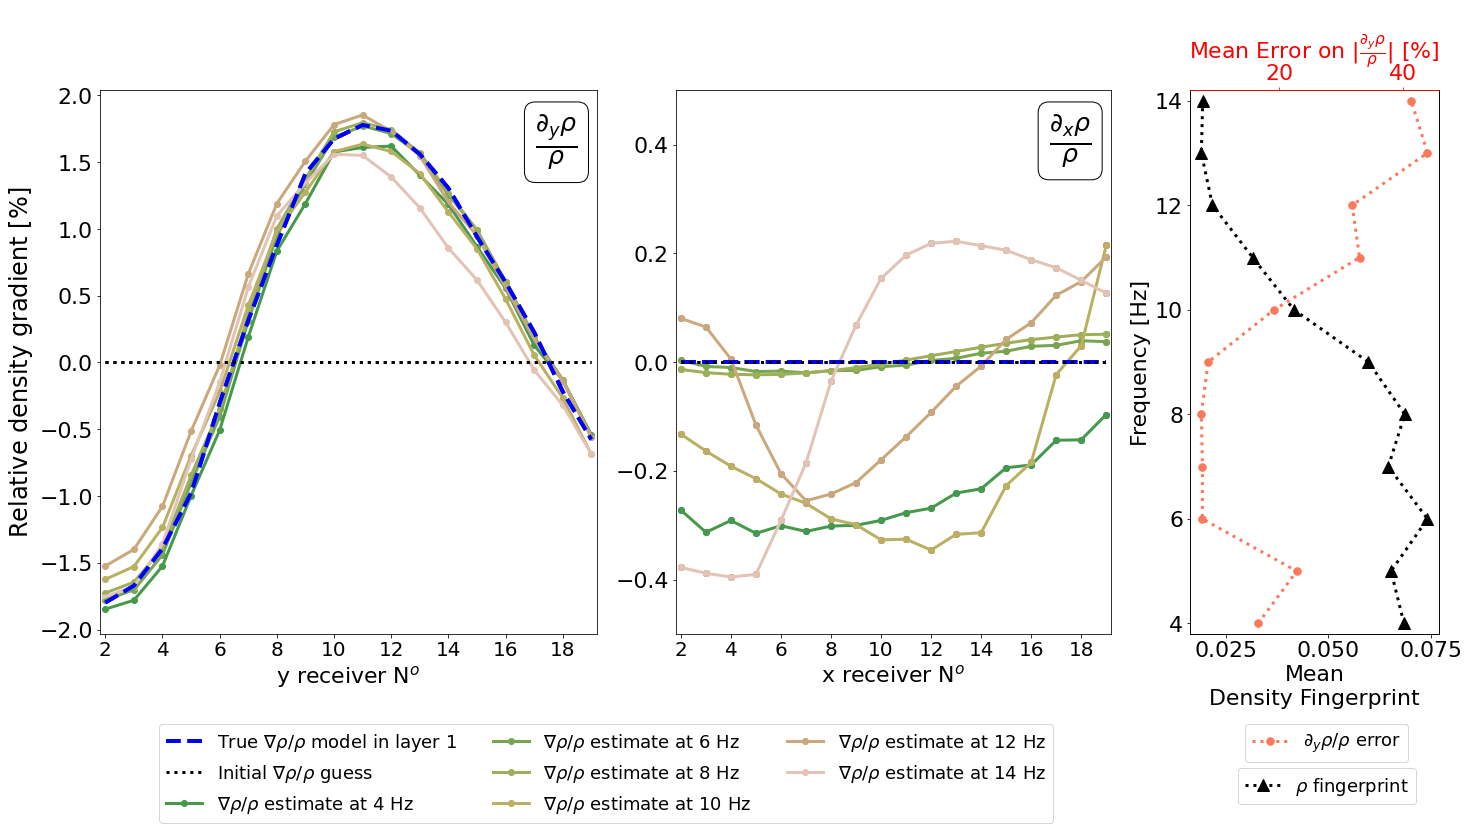
\includegraphics[width =\textwidth, keepaspectratio]{../Figures/freq_study_RHOgrad_REL.png}}
		\caption{Results for density inversion at the lowest misfit iteration for 2 Hz wide bandpasses around central frequencies 4 Hz, 6 Hz, 8 Hz, 10 Hz, 12 Hz and 14 Hz. Estimated density is shown as a mean over all x (left panel) and y (middle panel) cross-sections respectively. The right panel shows the mean error (Eq. \ref{eq:error}) on relative y-gradients of density averaged over the whole array per analysed frequency. The mean density fingerprint (Eq. \ref{eq:fingerprint}) is calculated for each frequency as $ 1/n_{t} \: \Sigma_{n=1}^{n_{t}} \: |\bm{\Gamma}_{n}|$ and then averaged over the array.}\label{fig:freq_rho}
	\end{figure}

	
	Figure \ref{dispersion}(d) shows how phase velocity perturbation increases with decreasing frequency and is roughly correlated with the signal strength of density. Full acoustic WEI can account for these density induced effects in phase velocity over a broad range of central filter frequencies, producing more accurate dispersion curves (Figs \ref{dispersion}a to \ref{dispersion}c). The full acoustic estimates display higher coefficients of determination (Fig. \ref{dispersion}b) and lower misfits (Fig. \ref{dispersion}c) than the Helmholtz results over all frequencies. As a reference we estimate a dispersion curve for the velocity model in Figure \ref{fig:TrueModel} with a constant density of 1600 $kg/m^{3}$ in layer 1 (Appendix \ref{sec:AppendixB}, Fig. \ref{fig:cst_rho}) and compare it to dispersion curves obtained with full acoustic and Helmholtz WEI (Fig. \ref{dispersion}a) for the variable density model (Fig. \ref{fig:TrueModel}). The dispersion curve calculated on the basis of full acoustic WEI is able to reproduce the general trend of the reference dispersion curve. We do not expect a perfect match as the imposed density structure in the laterally heterogeneous case does influence the paths taken by wave energy. The Helmholtz dispersion curve does not reproduce the key feature of a classical dispersion curve where phase velocity increases with decreasing frequency. This shows that it is detrimental for depth model reconstruction to assume a constant density over space in a medium with laterally heterogeneous density, especially at lower frequencies. % in discussion get back to this how useful this could be for more reliable 3D models and maybe cite a paper where there is a struggle with this..


	\begin{figure}[H]
		\centering
		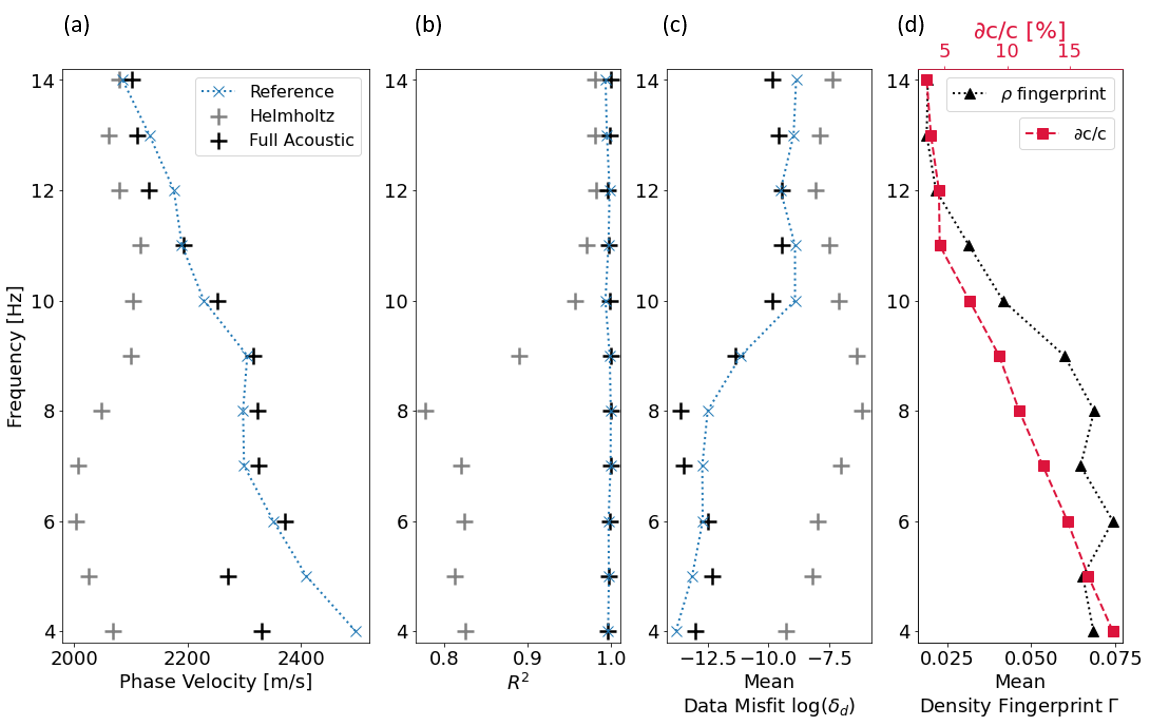
\includegraphics[width = 0.9\textwidth]{../Figures/disp_curve.png}
		\caption{Mean phase velocity dispersion curve (a) over the whole array obtained via Full Acoustic WEI (black crosses) and Helmholtz WEI (grey crosses) respectively. Phase velocity results are obtained for a reference model (blue dotted line with cross marker) produced by the same setup as described in Figure \ref{fig:TrueModel} but with constant density in layer 1 (Appendix \ref{sec:AppendixB}, Fig. \ref{fig:cst_rho}). Corresponding coefficients of determination (b) and misfits (c) are shown to evaluate the data fit. (d) The perturbation of phase velocity $\frac{\partial c}{c}$ (red dashed line with square markers) is defined by the difference between phase velocity in the heterogeneous (grey crosses) and homogeneous baseline model (blue crosses) obtained via linear regression on the basis of the Helmholtz wave equation. The mean fingerprint $\bm{\Gamma}$ of the density signal is defined as in Fig. \ref{fig:freq_rho} and shown by black triangles.} \label{dispersion}
	\end{figure}

	\subsubsection*{Random noise} \label{sec:rand_noise}	

	Given that in real use case scenarios WEI depends on field recordings, it is important to consider the robustness of density estimation to errors in the recorded signal. The density signal is relatively weak compared to that of phase velocity, hence it may be obscured by instrumentation noise in the field. We add random noise, expressed as a percentage of the mean trace amplitude over the whole grid, to the simulated observed signals in order to determine a threshold of noise beneath which the method still delivers meaningful results. For each receiver, the added noise follows an uncorrelated normal distribution with a spread of 0.1 to 5$\%$ of the mean trace amplitude.\\

	Correlation factors for density decrease with increasing noise levels. At noise levels 0.1 to 1$\%$ of the mean trace amplitude, the pressure with added noise remains relatively similar to the true pressure (Fig. \ref{fig:instrumental_noise}a). The density distributions are thus centred around the optimal correlation line where true and estimated density match perfectly (Fig. \ref{fig:instrumental_noise}b). At a random noise level of 5$\%$ the density distribution does not approximate the optimal correlation line well which suggests that the relative density structure cannot be estimated accurately. The correlation of phase velocity is dominated by the quality of the density information and vice-versa: correlation coefficient values follow the same deteriorating trend when the noise level becomes higher (Fig. \ref{fig:instrumental_noise}c). The estimates for both phase velocity and density remain stable up to a noise level of 1$\%$, but even at a noise level of 5$\%$ the main structural trends are still recognised.

	%\begin{figure}[H]
	%	\centering
	%	\includegraphics[width = 0.9\textwidth]{instrument_noise.png}
	%	\caption{text} \label{instrumental_noise}
	%\end{figure}

	\begin{figure}[H] \centering
	%\begin{tabular}[c]{c c}
	\hspace{0.00cm} \begin{subfigure}[c]{0.86\textwidth}
		\centering
		\subfloat[]{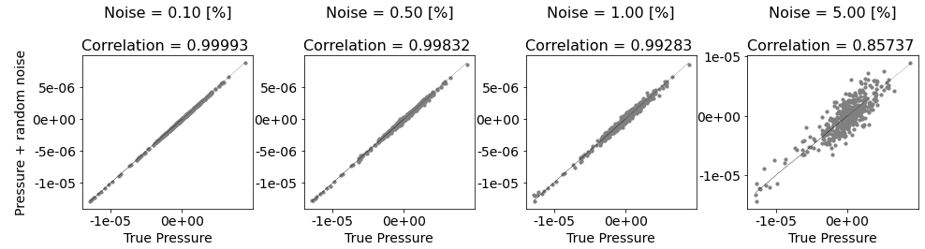
\includegraphics[width =\textwidth, keepaspectratio]{../Figures/instrument_noise_a.png}}
	\end{subfigure}\\
	\begin{subfigure}[c]{0.86\textwidth}
		\centering
		\subfloat[]{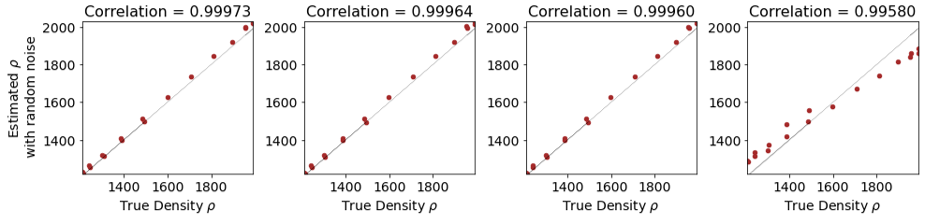
\includegraphics[width = \textwidth, keepaspectratio]{../Figures/instrument_noise_b.png}}
	\end{subfigure}
	\begin{subfigure}[c]{0.86\textwidth}
		\centering
		\subfloat[]{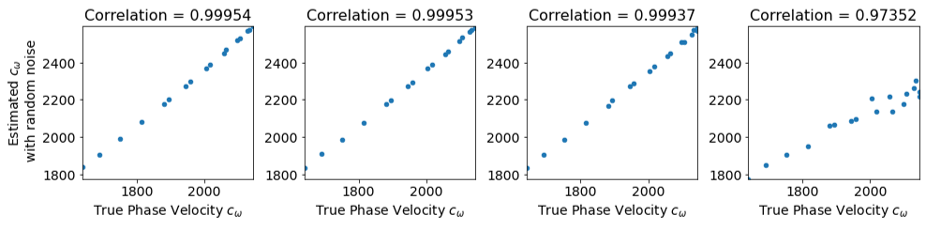
\includegraphics[width = \textwidth, keepaspectratio]{../Figures/instrument_noise_c.png}}
	\end{subfigure}
	\caption{(a) Correlation plots between true pressure signal and pressure signal with added random simulated instrumental noise at 0.1 $\%$, 0.5 $\%$, 1 $\%$  and 5 $\%$ of the mean amplitude of the modelled pressure signal over the whole grid. Wavefield arrivals at t>2s are used to visualise the effect of the added random noise on lower amplitude signals. Correlation plots of model material parameters at the various noise levels; between true and estimated (b) density and (c) phase velocity. True phase velocity is taken as $0.9v_{s}$ of the surface layer, hence the frequency dependance is not taken into account as it is difficult to determine the expected phase velocity in a laterally heterogeneous medium. }\label{fig:instrumental_noise}
	\end{figure}\mbox{}

	%\subsubsection*{Changing data frequencies} \label{sec:dispersion}
	%\newpage

	\subsubsection{Elastic Data} \label{sec:elasticRES} 

	%The effect of improving the misfit is very localized in time compared to the acoustic case (Figure \ref{XX}). By filtering the wavefield with a narrower bandpass, the signals originating from density effects become too weak to use within an inversion process. The inversion will try to fit the lowest misfit option and falls victim of the approximation effects: it tries to account for the 3D to 2D effect (even though minimal), the acoustic approximation of an elastic wavefield with the density effect being hidden somewhere within that signal. Neither the Helmholtz, nor the full acoustic description fit the wavefield well enough to distinguish a dominant clear density signal because of all the other approximations that are being done with the main culprit being trying to fit an acoustic equation onto an elastic field.
	The iterative full acoustic inversion procedure is performed in an elastic medium for the calculated wavefield potential $\Phi$ (from eq. \ref{eq:press_el}) for a central frequency of 8 Hz. The damping applied had to be 10 times stronger than in the acoustic case, with the damping factor at the initial stabilizing iteration equal to the mean amplitude of all recorded pressure signals. All subsequent iterations are carried out with 10$\%$ of the initial damping. The obtained results for density (Fig. \ref{fig:el_results}a) and relative density gradients (Fig. \ref{fig:el_results}b) suggest that the structural trends of the true model in the y-direction can be estimated approximately, but contain substantially more artefacts than in the acoustic case (Fig. \ref{fig:rho_est_8Hz}). The sinusoidal trend of the lateral heterogeneity in y-direction is recognisable but its shape is not approximated completely. These distortions are naturally also mapped into estimates of spatial density variations. The poorly constrained results in the x-direction demonstrate relative density gradients deviating from zero, especially between receiver 3 to 6  which does not agree with the constant true model. \\

	By examining the parameter error in x- and y-directions individually it becomes apparent that the parameter error in the x-direction monotonically increases with iterations, whereas the parameter error on the relative gradient in y-direction at first steadily decreases until iteration 60 after which it also follows an increasing trend. Consequently, artefacts are mapped into the density result during the inversion process. False structural density features are thus estimated by the inversion which suggests a strong cross-talk with other material parameters. A trade-off with velocity could cause the trend in velocity gradients in the x-direction, thereby distorting density. By mapping a false trend originating from the velocity error into the x-direction gradient, gradients in y-direction might compensate by over or under-estimating the density variation. The inversion being strongly influenced by the velocity response suggests that density has less weight in the elastic medium compared to the acoustic case. This becomes apparent in the misfit function map that explores the phase velocity and density space, displaying trade-offs between parameters in the acoustic and elastic case (Fig. \ref{fig:misfit_recLOC_main}). 

	\begin{figure}[H]  \vspace{-1.55cm} \centering
		%\begin{tabular}[c]{c}%{c}
		\hspace{0.00cm} \begin{subfigure}[c]{0.7\textwidth}
			\centering
			\subfloat[]{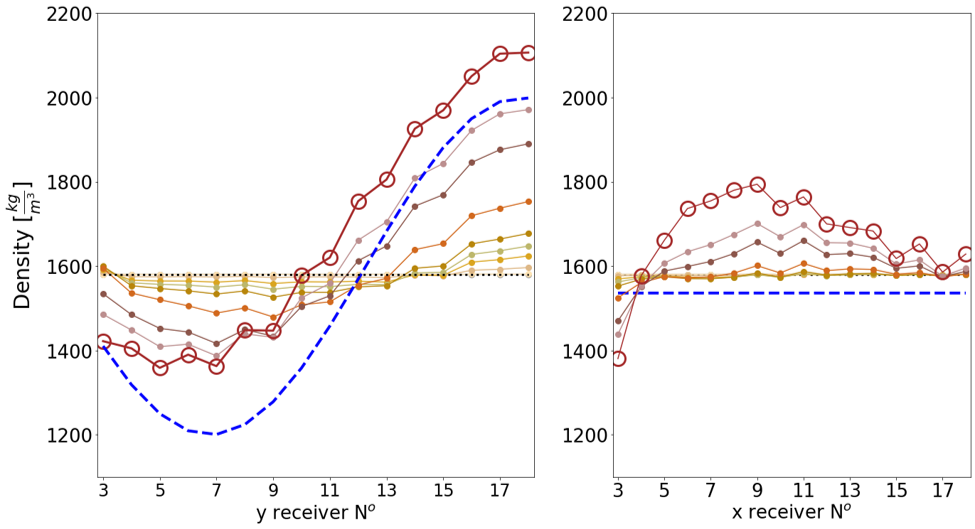
\includegraphics[width =\textwidth, keepaspectratio]{../Figures/EL_density_8Hz.png}}
		\end{subfigure}\\
		\begin{subfigure}[c]{0.683\textwidth}
			\centering
			\subfloat[]{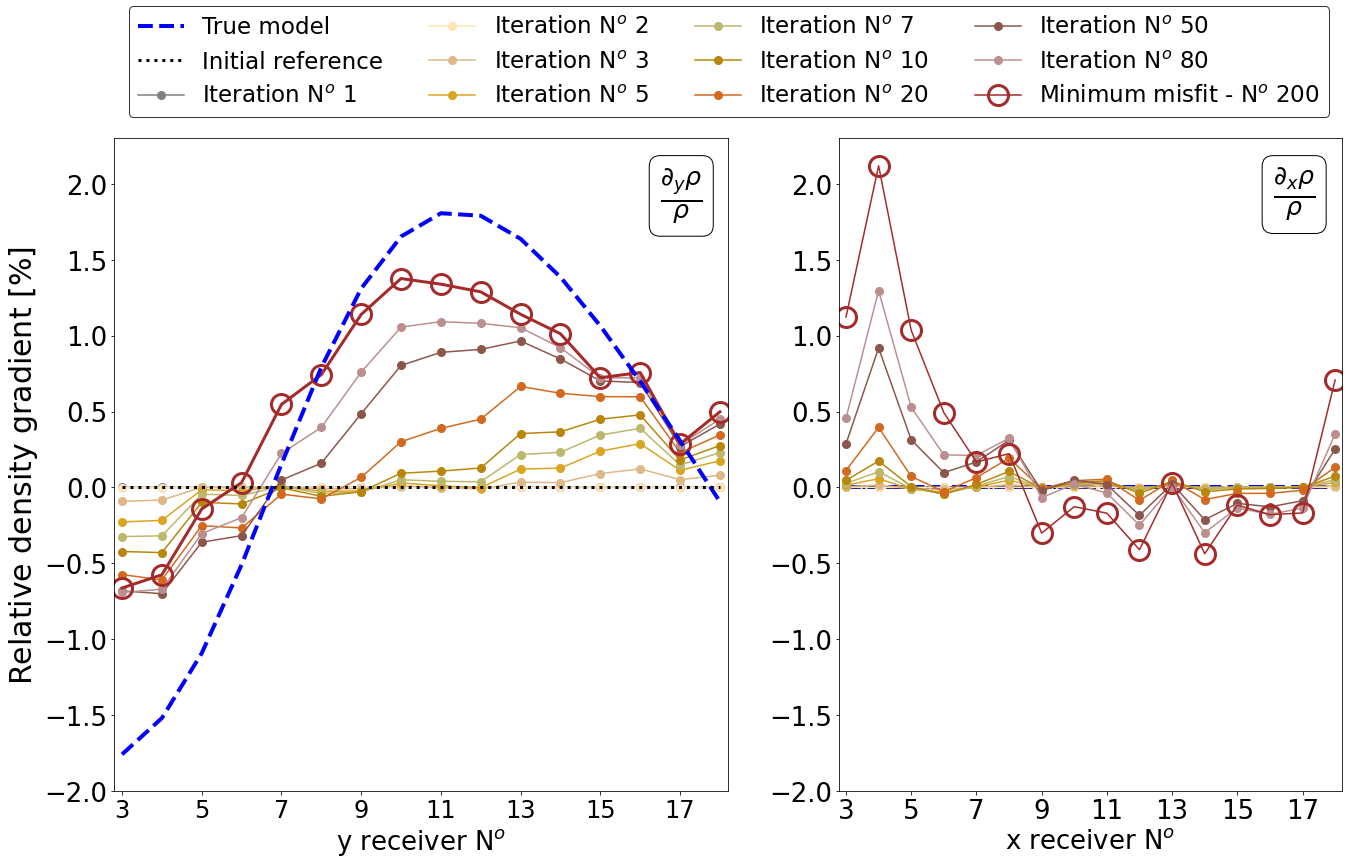
\includegraphics[width = \textwidth, keepaspectratio]{../Figures/EL_gradients_REL_8Hz.png}}
		\end{subfigure}
		\begin{subfigure}[c]{0.65\linewidth}
		\centering
		\subfloat[]{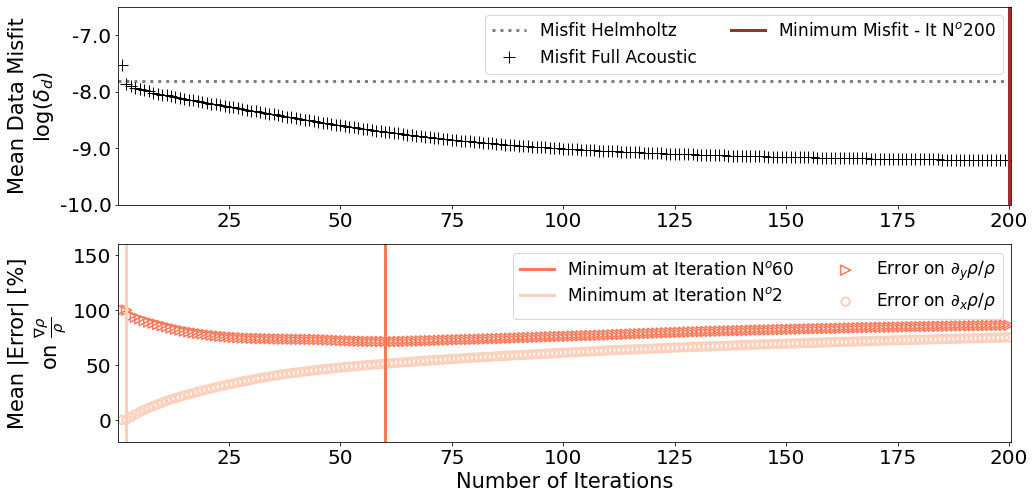
\includegraphics[width = \textwidth]{../Figures/iterations_min_ELASTIC_REL_8Hz.png}}
		\end{subfigure}
		%\end{tabular}
		\caption{Inversion result for an elastic wavefield filtered to include a frequency range between 7 Hz to 9 Hz. Only the results for the internal receivers 3 to 18 are displayed, as boundary stations need to be disregarded for finite difference estimates and computing pressure entails an additional differentiation step in approximating the divergence of the displacement. Mean value of inverted (a) density and (b) relative density gradient results over all cross-sections in x-plane (left) and y-plane (right) showing the evolution of the inversion at selected \DIFdelbeginFL \DIFdelFL{points }\DIFdelendFL \DIFaddbeginFL \DIFaddFL{stages }\DIFaddendFL during 200 iterations for a density model with sinusoidal heterogeneity as shown in Fig. \ref{fig:TrueModel}. True model is depicted as dashed dark blue line and initial model as dotted black line. The minimum misfit result coincides with the last iteration 200 and is highlighted by red circles. (c) Logarithm of the mean data misfit over all internal receivers (upper row) for the full acoustic wave equation (black crosses) over 200 iterations. As a reference, the misfit achieved with linear regression based on the Helmholtz equation is shown by the dotted grey line. Mean parameter error on x- and y- relative gradients is shown in the lower row over all internal receivers. The respective minimum value positions are marked by vertical lines in red for minimum misfit at iteration 200, dark orange and light orange at iteration 60 and 2 for minimum parameter error on relative density gradients in y-direction and x-direction. The minimum mean parameter error is evaluated after the initial stabilizing iteration. }
		\label{fig:el_results}
	\end{figure}

	 \subsubsection{Comparison between acoustic and elastic sensitivities} \label{sec:sensitivities}

	 To visualize the sensitivities of the inversion towards the investigated parameters, we perform a grid search where we analyse a grid of potential solutions for phase velocity and relative density gradients, and their misfit to the true model (Eq. \ref{eq:datamisfit}) at a fixed central receiver location $[x_{0},y_{0}]$ (Fig. \ref{fig:misfit_recLOC_main}). The density at the central location is fixed at the true value, but both neighbouring cells in the y-direction are freely variable in order to investigate the misfit evolution for various relative density gradient values. The density at $[y_{0}+1]$ and $[y_{0}-1]$ vary by $\pm$25 $\%$ around the true density value at $[x_{0},y_{0}]$ and produce relative gradient values between $\pm$6.25 $\%$. The phase velocity at the central point is variable around the phase velocity at $[x_{0},y_{0}]$ obtained by full acoustic WEI and spans a range of $\pm$25 $\%$. \\ %a mean value of the model phase velocity (taken at 0.9 $v_{s}$)

	 We compare the misfit function for acoustic and elastic wavefield data at the central frequency of 8 Hz. At the example receiver [13,13], the global misfit minimum is about 3 orders of magnitudes lower in the acoustic case than in the elastic one. This suggests that more uncertainty is attached to the inversion process in the elastic medium given that wavefield traces have been normalised prior to the evaluation.\\

	 The misfit function distribution in the acoustic medium shows that density gradients are better constrained than phase velocities (Fig. \ref{fig:misfit_recLOC_main}a): for logarithm misfit values within two order of magnitude from the minimum misfit (pink area, log($\delta_{d}$)<-11.4), the phase velocity can vary up to 4$\%$ whereas the relative density gradient is better constrained with no fluctuation at all \DIFaddbegin \DIFadd{over the applied binning}\DIFaddend . The absolute minimum misfit coincides exactly with the true value of the relative density gradient (|Error| = 0$\%$) and the minimum misfit phase velocity agrees well with the \DIFdelbegin \DIFdel{reference value of 2570m}\DIFdelend \DIFaddbegin \DIFadd{value of 2592m}\DIFaddend /s \DIFaddbegin \DIFadd{obtained via full acoustic WEI using the true density structure}\DIFaddend . All iterations from the inversion process plot very closely to the global misfit due to the strong constraints on both parameters.  \\

	 In elastic media, Figure \ref{fig:misfit_recLOC_main}(b) shows that a comparatively large number of relative density gradient and phase velocity values can explain the data on the basis of the full acoustic equation. For all solution pairs with misfit values within two orders of magnitude from the minimum misfit (pink to blue area on Fig. \ref{fig:misfit_recLOC_main}(b), log($\delta_{d}$)<-8.1), density gradients vary between 12.8$\%$ over the density gradient parameter space, whereas phase velocity fluctuates between 40.8$\%$ over the phase velocity parameter space. The comparatively higher uncertainty than in the acoustic case might be attributed to the weaker density signal strength (Fig. \ref{fig:rho_signal}) and approximations in physics. An error of 12$\%$ between the true relative gradient and the global misfit value suggests that the elastic data can not be fully explained by an underlying full acoustic wave equation. This implies that the inversion is prone to converge towards a slightly incorrect relative density gradient value.

	 \begin{figure}[H] \centering \hspace{0.00cm} 
	 	\begin{subfigure}[c]{0.6\textwidth}
	 		\centering
	 		\DIFdelbeginFL %DIFDELCMD < \subfloat[\normalsize Acoustic]{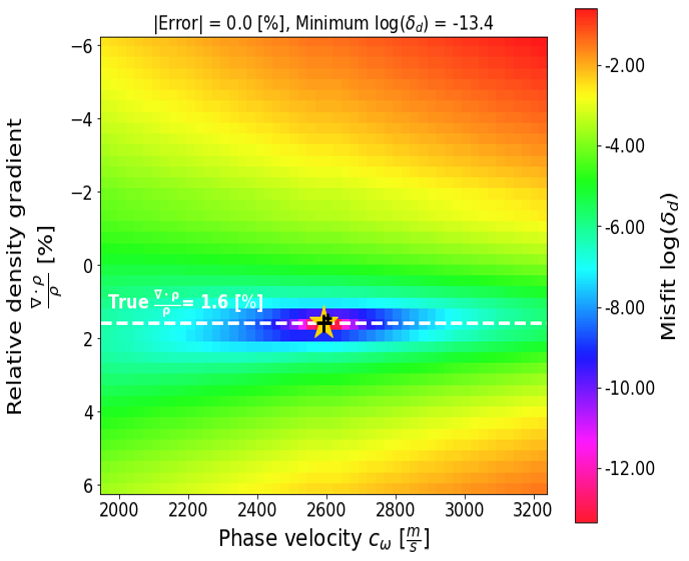
\includegraphics[width =\textwidth, keepaspectratio]{../Figures/ACC_misfit_8Hz_[12,12]_RAINBOW_noXY.png}}
%DIFDELCMD < 	 	%%%
\DIFdelendFL \DIFaddbeginFL \subfloat[\normalsize Acoustic]{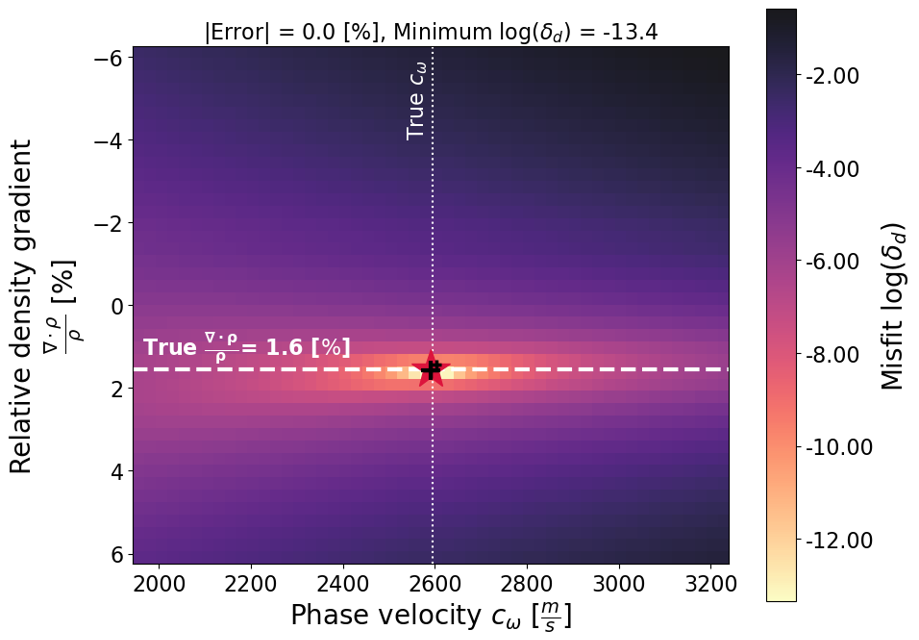
\includegraphics[width =\textwidth, keepaspectratio]{../Figures/ACC_misfit_8Hz_[12,12]_RAINBOW_noXY_magma_R_true.png}}
	 	\DIFaddendFL \end{subfigure}\\ \DIFaddbeginFL \DIFaddFL{\hspace{0.05cm}
	 	}\DIFaddendFL \begin{subfigure}[c]{0.6\textwidth}
	 		\centering 
	 		\DIFdelbeginFL %DIFDELCMD < \subfloat[\normalsize Elastic]{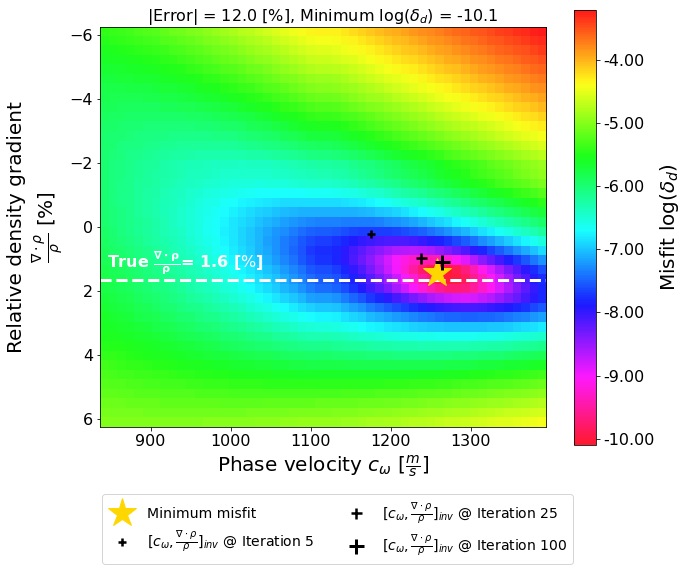
\includegraphics[width = \textwidth, keepaspectratio]{../Figures/EL_misfit_8Hz_[12,12]_RAINBOW_noXY.png}}
%DIFDELCMD < 	 	%%%
\DIFdelendFL \DIFaddbeginFL \subfloat[\normalsize Elastic]{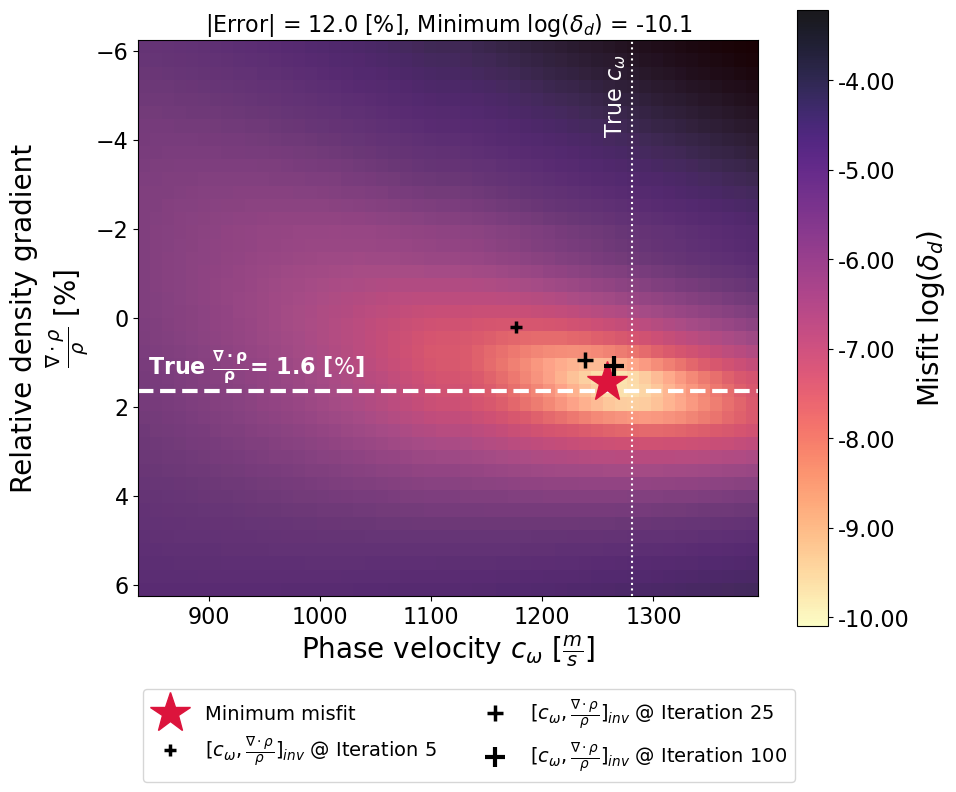
\includegraphics[width = \textwidth, keepaspectratio]{../Figures/EL_misfit_8Hz_[12,12]_RAINBOW_noXY_magma_R_true.png}}
	 	\DIFaddendFL \end{subfigure}
	 	\caption{Misfit functions for (a) acoustic and (b) elastic media at receiver location [13,13] for a central frequency of 8 Hz. The misfit function are representative of the data used to produce Figs \ref{fig:rho_est_8Hz} and \ref{fig:el_results} respectively. The |Error| (eq. \ref{eq:error}) shows the deviation of the relative density gradient value at the global minimum misfit in the grid search (yellow star) from the true value (white \DIFdelbeginFL \DIFdelFL{dotted }\DIFdelendFL \DIFaddbeginFL \DIFaddFL{dashed }\DIFaddendFL line). Misfit is calculated as defined in eq. \eqref{eq:datamisfit} and displayed for a single receiver. Crosses of increasing size show how total relative density gradient results of the iterative inversion process converges towards the global misfit of the grid search (small: iteration 5, medium: iteration 25, large: iteration 100). \DIFaddbeginFL \DIFaddFL{The true phase velocity $c_{\omega}$ (thin white dotted line) denotes the phase velocity obtained from full acoustic WEI when the true density structure is known .}\DIFaddendFL }%Iteration 100 is decomposed in x- and y-gradients marked by the respective letters x- and y- on the graph.
	 	\label{fig:misfit_recLOC_main}
	 \end{figure}

 	%paragraph actually belongs to the one above. just split for formatting reasons
	Iteration 5 of the inversion process gives an estimate on relative density gradient with a misfit value that is far away from the global misfit \DIFaddbegin \DIFadd{minimum }\DIFaddend (about two orders of magnitude) and provides a poor estimate on phase velocity and relative density gradient. Due to the comparatively poor constraints on both parameters, subsequent iterations are subject to parameter cross-talk and artefacts are mapped into the solution, corrupting primarily the relative gradient in the x-direction. Nevertheless, the inversion manages to converge towards a value in the vicinity of the true relative density gradient. To test the gradiometric estimate on phase velocity at the investigated receiver location, we use the surf-96 code (\cite{herrman84computer}) to calculate an expected value for mean Rayleigh wave velocity between 7 Hz to 9 Hz from the generated dispersion curve. The phase velocity value of 1260$m/s$ corresponding to the lowest misfit marked by the yellow star in Figure \ref{fig:misfit_recLOC_main}(b) is only 6$\%$ smaller than the expected value of 1340$m/s$ generated by a 2 layer model matching the 1D depth structure at the receiver location in our true model. \\%This might be explained by the fact that a severe approximation on the wave propagation physics of the elastic medium is used and that density contrasts do not play such an important role in longitudinal Rayleigh wave propagation. Alternatively, the highly oscillatory character of Rayleigh wave sensitivity to density might cause the density signals to be cancelled out.\\
	%The poor constraints on phase velocity might originate from the acoustic approximation

	%this shows that even by only measuring the pressure component of rayleigh waves, we do get good phase velocity estimates

	In summary, both acoustic and elastic media show sensitivity to relative density gradients. However, relative density gradients might not cause a large enough perturbation in the elastic wavefield to be sufficiently constrained in the inverse problem, whereas in acoustic media they are indeed essential to explain the data. \\

	\subsection{Volumetric arrays} \label{sec:vol_res}
	\subsubsection{Elastic Data} \DIFaddbegin \label{sec:vol_res_el}
	\DIFaddend 

	In a first step using a volumetric array, body wave velocities are estimated for a wavefield filtered between 7 Hz to 9 Hz using a least-squares inversion from eq. \eqref{eq:freeSurfT}. Those velocity results (Fig. \ref{fig:FS_rho}a) are substituted into equations \eqref{eq:FS_discr_LHS} to \eqref{eq:FS_discr_RHS} along with the calculated pressure. Pressure at the free surface is given in eq. \eqref{eq:PRESS_edme}, but we find that using only the related acoustic expression \DIFdelbegin \DIFdel{$P = K_{a} \nabla_{H}\cdot \bm{u}^{H}$ }\DIFdelend \DIFaddbegin \DIFadd{$P = K_{a} \nabla_{H}\cdot \bm{u}_{H}$ }\DIFaddend delivers more reasonable inversion results for density. Figure \ref{fig:FS_rho} shows the estimated density results obtained by linear regression of eq. \eqref{eq:FS_RHO_linREG}. The accuracy of the density results depends on how well the velocities can be estimated. The mean value of the absolute parameter error over the receiver grid (Fig. \ref{fig:FS_rho}b, right) measures 3.04 $\%$ illustrating that the estimated results are close to the true parameter values. Once body wave velocities and densities are estimated, we can procede to calculate  Lam${\'e}$ parameters via empirical relationships: results are shown for the first Lam${\'e}$ parameter in Fig. \ref{fig:FS_rho}(c). \\

	%To illustrate how the density problem is constrained, we perform a misfit analysis of potential solutions for density and body wave velocities. The left-hand side of \eqref{eq:FS_RHO_linREG} is %fixed at the estimated body wave velocity values. On the right-hand side, both density and velocity vary by $\pm 50\%$ around their true value but P and S wave velocities have a fixed Poisson ratio 

		\begin{figure}[H] \centering
		\begin{subfigure}[c]{0.8\textwidth}
			\centering
			\subfloat[]{\includegraphics[width =\textwidth, keepaspectratio]{../Figures/FS_velocity_result.png}}
		\end{subfigure}\\
		\begin{subfigure}[c]{0.8\textwidth}
			\centering
			\subfloat[]{\includegraphics[width = \textwidth, keepaspectratio]{../Figures/FS_rho_result.png}}
		\end{subfigure}\\
		\begin{subfigure}[c]{0.8\linewidth}
			\centering
			\subfloat[]{\includegraphics[width = \textwidth]{../Figures/FS_lam_result.png}}
		\end{subfigure}
		\caption{Plan view of (left column) true model and (middle column) gradiometric estimates of material parameters. The corresponding parameter error (Eq. \ref{eq:error}) is shown in the right column. Rows (a), (b) and (c) correspond to results for P wave velocity, density and the first Lam${\'e}$ parameter $\lambda$. Velocities are estimated via WEI of eq. \ref{eq:freeSurfT}, densities by linear regression of eq. \eqref{eq:FS_RHO_linREG} and Lam${\'e}$ parameters are obtained from the latter estimated velocity and density results where $\lambda = (v_{P}^{2} - 2v_{S}^{2}) \rho$.} \label{fig:FS_rho}
		\end{figure}\label{fig:FS_elastic_results}


	% \begin{figure}[H] 
	%	\centering
	%	{\includegraphics[width =0.6\textwidth, keepaspectratio]{FS_misfit_rho_vp.png}}
	%	\caption{Misfit function for elastic media at receiver location [13,13] for a central frequency of 8 Hz. The misfit function are representative of the data used to produce Fig. %\ref{fig:FS_elastic_results}. The |Error| (eq. \ref{eq:error}) shows the deviation of the density value at the global minimum misfit in the grid search (yellow star) from the true value (white %dotted line). Misfit is calculated as defined in eq. \eqref{eq:datamisfit} and displayed for a single receiver.}
	%	\label{fig:FS_rho_misfit}
	%\end{figure}

	%\newpage
	\section{Discussion}
	We have shown that in acoustic media, relative density gradients of 1.6$\%$ produce a substantial change in the synthetic wavefield. This allows us to set up an inverse problem that successfully estimates density structure of the medium. \DIFaddbegin \DIFadd{The WEI approach has been demonstrated both at the example of models where density and velocity structure are fully uncorrelated, as well as structurally more common models that approximate geological interfaces. }\DIFaddend Density contrasts down to the amplitude of  0.5$\%$ can be imaged with a parameter error smaller than 10$\%$ (Figure \ref{fig:damping}). First tests suggest that the inversion process is robust for random noise up to 1$\%$ of the mean trace amplitude (Fig. \ref{fig:instrumental_noise}) which encourages a future trial on real data.\\

	In elastic media, other effects interfere with the density signal, making density estimation more difficult from surface array data alone. Elastic results (Section \ref{sec:elasticRES}) and sensitivity analysis (Section \ref{sec:sensitivities}) show that there is sensitivity to relative density gradients in elastic media. However, the full acoustic approximation is too severe for elastic wave physics and density is too weakly constrained to be fully estimated using the proposed iterative inversion process. This makes it unlikely that density inversion based on gradiometric full-acoustic WEI will be feasible in an elastic Earth, or worse a visco-elastic Earth where the already small density signal might be overshadowed by the additional medium parameter of energy dissipation. The method might only be applicable in localized areas where the wavefield passes predominantly through gas or liquids.\\

	To estimate density in elastic media it is therefore necessary to use volumetric array measurements and to adopt a more accurate representation of underlying wave physics as a basis for gradiometric WEI, such as the full elastic wave equation. However, it became clear from equation \eqref{eq3a} that if we only measure particle velocity or displacement and if the source term $\bm{f}$ is omitted, density does not appear as an independent term outside of the expressions for body wave velocity. It is therefore impossible to estimate density independently of the Lam${\'e}$ parameters using a sourceless full elastic equation. However, if both displacement and pressure are measured in a dual sensor configuration, the full elastic wave equation at the free surface exhibits a direct, independent sensitivity to density in the form of a linear relationship between pressure and displacement terms (Section \ref{sec:vol_res}). If we are willing to deploy buried receivers then the results herein suggest that density can be estimated directly from recorded data, together with P and S velocities. Pressure sensors for solid earth applications have been presented as a prototype (\cite{edme2018seismic}), but reliable pressure measurements are not readily available as of yet.\\

	While our focus herein has been to make use of the ambient wavefield, an alternative exists if we consider the introduction of a local source within the receiver array. In that case, if the associated body force term $\bm{f}$ is clearly defined, density can be isolated within the wave equation and could in theory be estimated. We therefore propose a thought experiment in which we consider a weight drop within a 3D gradiometric receiver array (Fig. \ref{fig:gradio_types}a) and perform volumetric gradiometry. If we assume that the weight drop acts as a vertical point load on the surface then the body force $\bm{f}$ is generally defined as a distribution of force density as a function of position and time (\cite{madariaga2007seismic}):
	\begin{align}\shoveright \shoveright \shoveright \shoveright \shoveright \shoveright \shoveright \shoveright \shoveright \shoveright \shoveright
		\bm{f}(\bm{x},t) = \bm{f_{0}} \: s(t) \: \delta(\bm{x}-\bm{x_{0}}) 
	\end{align}
	where  $\bm{f_{0}}$ is a unit vector in the direction of the point force $\bm{f_{0}} = [0,0,1]^{T}$, $s(t)$ is a source time function (the variation of
	the amplitude of the force as a function of time) applied in the vertical direction and $\delta(\bm{x}-\bm{x_{0}})$ is the Dirac distribution centered at the source location $\bm{x}_{0}$. \textcite{neitzel1958seismic} first analysed the seismic characteristics of a weight-drop source in a field experiment: he measured the force applied to the ground in an effort to characterise the source term and recorded the wavefield response. Several authors thereafter proposed source term expressions to explain wavefield observations produced by a weight drop: based on the work of \textcite{lamb1904propagation}, \textcite{pekeris1955seismic} and \textcite{mooney1974some} derived analytical expressions of the wavefield response at the free surface due to the application of an arbitrary excitation. The use of Heaviside step function and Dirac Delta function could not reproduce wavefield quantities accurately, whereas a sinusoidal source time function was shown to better approximate the generated wavefield (\cite{abe1990seismic}).  Defining a generalised source term as accurately as possible is an essential task in predicting the Earth response to a weight drop, and hence also in the proposed application to gradiometry. \textcite{colombero2015numerical} found that the source time function in the near-field of a weight drop can be represented by a modified Gabor wavelet (based on \textcite{semblat2009waves}) expressed in terms of particle velocity:
	\begin{align}\shoveright \shoveright \shoveright \shoveright \shoveright \shoveright \shoveright \shoveright \label{eq:Gabor}
		s(t) = \begin{cases}
			C_{b} \: \beta \: t^{\gamma} \: exp[-(\frac{2 \pi }{T_{s} \: \alpha}t)^{2}] \: cos(\frac{2 \pi }{T_{s}}t) & \text{if $0 \le t \le 1.2 T_{s}$}\\
			0 & \text{otherwise}
		\end{cases}     
	\end{align}\mbox{}

	where t is a generic time instant, $T_{s}$ the period of the function, $C_{b}$ the momentum of the dropped weight and $\alpha$, $\beta$ and $\gamma$ are constants whose corresponding values are given in \textcite{colombero2015numerical}. By comparing recorded particle velocity from drop load tests and synthetic data generated by propagating the proposed source signal, they found that simulated and real impulse responses in the near-field of the source match well. \\ %over the extent of a finite difference stencil

	We therefore propose that in the case where we allow ourselves the luxury of a local source, the modified Gabor source time wavelet (eq. \ref{eq:Gabor}) could in principle be incorporated in the volumetric gradiometry workflow in order to estimate density on the basis of the full elastic wave equation at the free surface. \DIFaddbegin \DIFadd{Alternatively, one could use a piezoelectric sensor as a controlled source using a preset electrical current signal (e.g., a Ricker wavelet) to drive the resulting vibrations at the source point in the form of a known source time function. }\DIFaddend In a first step we consider equation \eqref{eq3a} without body forces. We can then estimate P-wave velocity $v_{P,e}$ and S-wave velocity $v_{S,e}$ at the free surface for any incoming wavefield using volumetric gradiometric measurements and the Lax-Wendroff correction (\cite{lax1964difference}) as proposed by \textcite{curtis2002volumetric}. Then by applying body forces in the form of a weight drop where s(t) is clearly defined (eq. \ref{eq:Gabor}), equation \eqref{eq:freeSurfT} that describes the vertical component of a wavefield $\bm{\theta}=[\theta_{x}, \theta_{y}, \theta_{z}]$ at the free surface takes the form:
	\begin{align} \shoveright \shoveright \shoveright \shoveright \shoveright \shoveright 
 		[\partial_{t}^{2} \: \theta_{z} - v_{P,e}^{2} \: A_{z}(t) \: + \: v_{S,e}^{2} \: B_{z}(t)]   \: \rho	\: = \DIFdelbegin %DIFDELCMD < \bm{f}
%DIFDELCMD < 		%%%
\DIFdelend \DIFaddbegin \DIFadd{f_{z}
		}\DIFaddend \label{eq:freeSurf}   
	\end{align} 
	%\begin{align} \shoveright \shoveright \shoveright \shoveright \shoveright \shoveright 
	% v_{P,e}^{2} \: A_{z}(t) \: - \: v_{S,e}^{2} \: B_{z}(t)  	\: = \partial_{t}^{2} \: \theta_{z}
	%\label{eq:freeSurf0}   
	%\end{align} 
	with $A_{z}(t)$ and $B_{z}(t)$ given in equations \eqref{eq:Az} to \eqref{eq:Bz}. %being expressions containing finite difference approximations to derivatives of the wavefield
	%\begin{align} \shoveright \shoveright \shoveright \shoveright \shoveright \shoveright 
	%	A_{z}(t)  	\: &= \:   \frac{2}{\Delta z} \big(\nabla_{H} \cdot \bm{\theta}_{H} + [\partial_{z} \theta_{z}]_{fd} \big) \: - \: \nabla^{2}_{H} \theta_{z} \\
	%	B_{z}(t) 	\: &= \:   \frac{4}{\Delta z} \big(\nabla_{H} \cdot \bm{\theta}_{H}\big) \: - \: 2\big(\nabla^{2}_{H}\theta_{z}\big)
	%	\label{eq:++}   
	%\end{align}
	%where $\Delta z$ is the distance between the surface and the buried receiver and $[\partial_{z} \theta_{z}]_{fd}$ is the first order finite difference depth derivative. These expressions are obtained by applying the Lax-Wendroff correction scheme in order to correctly represent the first order finite difference derivative of the wavefield in depth at the free surface. The derivation of these expressions is described in detail in \textcite{curtis2002volumetric}. 
	The entire left-hand side of equation \eqref{eq:freeSurf} is then known apart from density, and takes the form of a linear inverse problem which might be solved for density. \\

	Theoretically the response at the buried receiver could be inferred analytically by Green's function retrieval, if the effective volume encompassed by the gradiometric 3D receiver array is considered a uniform half-space in accordance with Lamb's problem. \textcite{johnson1974green} and \textcite{chen2020green} provide an expression of the Green's function at a buried receiver for a surface source over a homogeneous half-space. By extending this work to a Gabor wavelet source time function, the wavefield response at a buried receiver could be written analytically, reducing the acquisition requirements to a surface array.

	%%n the frame of Lamb's problem, several authors analysed the wavefield generated by a point source at the surface over a homogeneous half-space (Pekeris, Mooney,...)

	%In Section (\ref{sec:theory}), we mention the different roles that density plays in elastic and acoustic media respectively at the example of their governing wave equations. Changes in density are only caused by dilatational changes to the medium. They are related to pressure changes which correspond to a change in volume of the medium and are proportional to the divergence of the displacement field. Rotational parts of the wavefield do not exhibit this same sensitivity to density and thus their propagation is poorly approximated by the full acoustic wave equation. We showed that in acoustic media, where wave propagation purely happens by compression and dilatation, wavefield gradients exhibit a direct sensitivity to density (Equation (\ref{eq3b})).\\

	%A diffracted pressure field caused by a density perturbation is contained in the incident wave field (\cite{tarantola1984inversion}). In our 3D acoustic synthetic tests, it was possible to capture the signal of the diffracted pressure field caused by lateral variations in density and thus invert for the relative density structure. In elastic media, density also shows to have an independant expression only for the dilatational part of the wavefield and if the measured wavefield quantity is equivalent to the acoustic pressure. By approximating seismic surface waves in elastic media by acoustic waves however, not only mode conversions , but also the directivity of scattering from a point of heterogeneity are neglected (\cite{wielandt2}). In reality however, scattering angles are heavily dependant on the wave type and what causes them: density affects the seismic wavefield mainly through reflection/backscattering (\cite{wu_scatter}). The strength of the density signal might depend on the angle of incidence upon reflection, e.g. how much P-wave energy is reflected (Fig. 3.2. (a) in (\cite{sheriff1995exploration})) and reaches the receivers. \\

	%Furthermore, the contribution of a density anomaly to an observed wavefield change depends on the scattering angle of the back-scattered energy that reaches the receiver. This is due to the fact that at certain scattering angles, the density and velocity signals overlap more or less strongly (\cite{luo2018velocity}). Density has a radiation pattern which shows a maximum sensitivity of causing a change in the wavefield at the zero scattering angle, but a wavefield change associated with one parameter class can be affected by crosstalk from one or more other parameter classes (\cite{operto2013guided}). The sensitivity to the density induced partial derivative wavfield gradually decreases with scattering angle to zero at the $180^{o}$ scattering angle (\cite{prieux2013multiparameter}). This radiation pattern causes particularly strong trade-offs with velocities at short- to intermediate-scattering angles. In full waveform inversion this issue is mitigated by moving to a velocity-impedance parametrization (\cite{prieux2013multiparameter}; \cite{operto_miniussi}). (\cite{luo2018velocity}) tries to minimize this effect by inverting for angle-separated data. %needs more paraphrasing, 2 different points: sensitivity to gradient, and bas trade offs, but why not in acoustic case............
	%Scattering patterns are more complex in elastic media than in acoustic media because of the presence of different wave types (\cite{tarantola1986strategy}; \cite{wu_scatter}; \cite{beller2018lithospheric}). Different wave types are more or less sensitive to different material parameters. This increased complexity and interference of radiation patterns caused by subsurface elastic parameters, medium speed or density might explain why density inversion in the elastic simulations delivers poorer results with stronger trade-offs than in the acoustic case. Velocity or the elastic parameters have different effects on wave amplitudes and phases than density, so if most of the recorded wavefield contains signals from velocity scattering or Lame parameter scattering, the density is overshadowed. \\

	%Our sensitivity analysis (Section \ref{sec:sensitivities}) suggests that the full acoustic approximation is too severe of an approximation of elastic wave physics and that the density is too weakly constrained to fully estimate it with the proposed iterative inversion process. Discriminating wavefield arrivals by scattering angle (\cite{luo2018velocity}) might help select parts of the wavefield that are uniquely sensitive to density and thus better inform our proposed density inversion.  Furthermore, fingerprinting of different wave types in ambient noise traces (\cite{sollberger2023efficient}) would allow to extract any desired wavefield arrival and analyse their respective sensitivities to density. Selecting wave types with high sensitivity might help improve the inversion process. Moreover, at this stage, our analysis is limited to purely acoustic or purely elastic media. In media that have a strong acoustic imprint on the wavefield such as soils that are highly saturated with water or CO2 storage reservoirs, density might play a larger role in wavefield amplitude and phase to become detectable.\\

	 %(\cite{blom2017synthetic}) write that density anomalies at the order of 10 $\%$  produce a change in wavefield amplitude of 5 $\%$ which is large enough to be measurable with current state-of the-art broad-band sensors. We showed that in acoustic media, relative gradients of 1.6$\%$ over the finite difference stencil were easily picked up in our synthetic examples, whereas it becomes more difficult for density contrasts below  0.5$\%$ (Figure (\ref{fig:misfit})). First tests suggest that the inversion process is robust for random noise up to 1 $\%$ of the mean trace amplitude which is encouraging to trial the method on real data. In elastic media, other effects are interfering with the signal from the density contrasts, making it more difficult to be estimated: (\cite{blom2020seismic}) characterize density to be the inversion's 'garbage bin'. This makes it unlikely for density inversion based on gradiometric full-acoustic WEI to be feasible in an elastic Earth, or worse visco-elastic Earth where the already small density signal might be overshadowed by the additional media parameter of energy dissipation. The method might only be applicable in localized areas where the wavefield passes predominantly through gas or liquids in the subsurface.\\

	
	

	%\newpage
	\section{Conclusion}
	We investigated whether surface wavefield gradiometry can be used to gain insights into material density via WEI of the full acoustic wave equation in both 3D acoustic as well as 3D elastic media using ambient noise data.  We propose and test an iterative inversion scheme for both density and phase velocity based on gradiometric WEI and simulated ambient noise. No inherent scaling between velocity and density is imposed, making it suitable to detect density changes caused by temperature or chemically induced mechanisms. Synthetic results for 3D acoustic media suggest that it is possible to estimate relative density structure with WEI by using a full acoustic formulation for wave propagation along the surface. We show that using a constant density assumption for the medium can be detrimental to subsurface velocity images, whereas the full acoustic formulation of gradiometry improves our knowledge of all material properties. It allows us to estimate density as an additional material parameter as well as to improve phase velocity estimates by incorporating approximations of the density structure.\\

	By expanding this methodology to the elastic case, we tested the feasibility of estimating density in the solid Earth with gradiometric WEI on the basis of a full acoustic approximation. The dilatational component of Rayleigh waves at the free surface was shown to be imprinted by effects from relative density changes in the medium. It proved however to be more difficult to obtain reliable estimates on relative density changes in elastic media than in acoustic media due to a stronger trade-off between density and phase velocity caused by the difference in the measured wave type sensitivities to material parameters in both analysed media. However, using a 3D array and the full elastic wave equation at the free surface it is possible to obtain reliable \DIFaddbegin \DIFadd{absolute }\DIFaddend density estimates in elastic media. We suggest that another reasonable way to obtain density estimates in elastic media would be to fire a local source and include the corresponding source term within an inversion of the full elastic wave equation.

	%By expanding this methodology to the elastic case, we tested the feasibility of estimating density with gradiometric WEI in the solid Earth and found that density corrupts the phase velocity estimate based on the Helmholtz wave equation way less significantly than in the acoustic case. To be able to estimate a decoupled density signal in elastic media, we need to approximate the solid Earth as an acoustic body.\\

	%gradiometry insight into density gradients
	\section*{Acknowledgements}

	The present project was supported by the National Research Fund (FNR) of Luxembourg and by a Doctoral Training Partnership grant (NE/S007407/1) from the UK Natural Environment Research Council (NERC). \DIFaddbegin \DIFadd{The authors thank David Sollberger and one anonymous reviewer for their thoughtful comments that helped to improve the manuscript, as well as, Fern Storey and Andrew Valentine for editorial handling. 
	 }\DIFaddend 

	\section*{Data Availability} 
	\hypersetup{
		colorlinks=true,
		linkcolor=blue,      
		urlcolor=cyan,
	}

	\DIFdelbegin \DIFdel{All code and synthetic data }\DIFdelend %DIF > All code and synthetic data used in this study can be shared with any interested party on request to the corresponding author.
	\DIFaddbegin \DIFadd{All code }\DIFaddend used in this study \DIFdelbegin \DIFdel{can be shared with any interested party on request to the corresponding author. 
	%DIF < All code used in this study are publicly available at \url{https://github.com/mafab1994/density_WEI}. The synthetic data used in this work can be shared with any interested party on request to the %corresponding author.
	}\DIFdelend \DIFaddbegin \DIFadd{is publicly available at }\url{https://github.com/mafab1994/density_WEI}\DIFadd{. The synthetic data was produced with the Salvus software package from Mondaic AG and is made available on the Zenodo repository }\url{https://doi.org/10.5281/zenodo.10474217}\DIFadd{. 
	%DIF > The synthetic data used in this work can be shared with any interested party on request to the %corresponding author.
	}\DIFaddend 

	\DIFdelbegin %DIFDELCMD < \newpage
%DIFDELCMD < 	%%%
\DIFdelend %DIF > \newpage

	% \section{References}
	\singlespacing
	\begin{multicols}{2}[\printbibheading]
	\printbibliography[heading=none]
	\end{multicols}

	\doublespacing
	\newpage
	\DIFaddbegin 

	\DIFaddend \appendix

	\section*{Appendix} 
	\renewcommand{\thesubsection}{\Alph{subsection}}
	\subsection{Finite Difference Error}\label{sec:Appendix}
	\renewcommand{\theequation}{A\thesection\arabic{equation}}
	\setcounter{equation}{0}
	\renewcommand{\thefigure}{A\arabic{figure}}
	\setcounter{figure}{0} 

	Throughout this analysis we use $2^{nd}$ order accurate formulations of the finite difference approximation of the $2^{nd}$ spatial derivative of the wavefield quantity $\theta$:
	\begin{equation}
		\frac{\partial^{2} \theta}{\partial x^{2}} \: = \: \frac{\theta(x-\Delta x) - 2 \theta(x) + \theta(x+ \Delta x)}{\Delta x^{2}} -  \frac{\Delta x^{2}}{24} \frac{\partial^{4} \theta}{\partial x^{4}}
	\end{equation}
	Following (\cite{Langston1}) we can calculate the error of this approximation due to the sampling for a sinusoidal wave by assuming a plane wave in the form
	\begin{equation}
		\theta(x,t) = e^{i \omega (t-\frac{x}{c})}
	\end{equation}
	We can then calculate the error $\epsilon$ based on the following formulation:
	\begin{equation}
		\epsilon = \left| \DIFdelbegin \DIFdel{\frac{-\frac{1}{24} \frac{\partial^{4} \theta}{\partial x^{4}}}{\frac{\partial^{2} \theta}{\partial x^{2}}} }\DIFdelend \DIFaddbegin \DIFadd{\frac{-\frac{\Delta x^{2}}{24} \frac{\partial^{4} \theta}{\partial x^{4}}}{\frac{\partial^{2} \theta}{\partial x^{2}}} }\DIFaddend \right| \: = \: \frac{\Delta x^{2} (2 \pi)^{2}}{24 \lambda^{2}}
	\end{equation}
	Setting an accuracy threshold $\zeta$ for the second derivative, the condition
	\begin{equation}
		\epsilon \le \zeta \Leftrightarrow \Delta x \le \sqrt{\frac{\zeta \: 24 \lambda^{2}}{(2 \pi)^{2}}}
	\end{equation}
	implies the spacing $\Delta x$ needs to be at \DIFdelbegin \DIFdel{least }\DIFdelend \DIFaddbegin \DIFadd{most }\DIFaddend 0.247 $\lambda$ to ensure an error lower than $\zeta=0.1$.

	\begin{figure}[H]
		\centering
		\includegraphics[width =0.5\linewidth]{../Figures/error.png}
		\captionsetup{width=\linewidth}
		\caption{Error evolution of the used Finite Difference approximation with frequency for different receiver spacings given in m. Black dotted line shows threshold error of 10 $\%$.}
		\label{fig:error}
	\end{figure}

	\newpage

	\subsection{Reference Density Model} \label{sec:AppendixB}
	\renewcommand{\thefigure}{B\arabic{figure}}
	\setcounter{figure}{0} 
	\begin{figure}[H]
		\centering
		\includegraphics[width =0.65\linewidth]{../Figures/rho_constant.png}
		\captionsetup{width=\linewidth}
		\caption{Reference density model depth cross-section in yz-plane. A constant density of 1600 $kg/m^{3}$ is used for the top layer instead of the variable density structure imposed in Figure \ref{fig:TrueModel}c and \ref{fig:TrueModel}d. 1600 $kg/m^{3}$ corresponds to the mean value of the top layer in the variable density model.}
		\label{fig:cst_rho}
	\end{figure}\mbox{}

	\subsection{\DIFdelbegin \DIFdel{Notes on the free surface methodology in inhomogeneous elastic media}\DIFdelend \DIFaddbegin \DIFadd{Frequency Dependence of Absolute Density Estimate}\DIFaddend } \DIFdelbegin %DIFDELCMD < \label{sec:AppendixC}
%DIFDELCMD < 	%%%
\DIFdelend \DIFaddbegin \label{sec:APP_FREQ}
	\DIFaddend \renewcommand{\theequation}{C\thesection\arabic{equation}}
	\setcounter{equation}{0}
	\renewcommand{\thefigure}{C\arabic{figure}}
	\setcounter{figure}{0} 
		\DIFaddbegin \begin{figure}[H]
		\centering
		\includegraphics[width =0.55\linewidth]{../Figures/abs_rho_Freq.png}
		\captionsetup{width=\linewidth}
		\caption{\DIFaddFL{Frequency dependence of absolute density estimates obtained from full acoustic wave equation inversion. True model values shown at two local stations highlighted in Figure \ref{fig:c_est_8Hz} e.g., }[\DIFaddFL{13,13}] \DIFaddFL{(green dotted line) and }[\DIFaddFL{13,6}] \DIFaddFL{(red dotted line) and as a mean over all stations (dark blue dotted line). Estimates are shown as crosses in the respective corresponding colours. The light blue dotted line shows the density value of layer 2. }}
		\label{fig:abs_rho_FREQ}
		\end{figure}%DIF > \mbox{}

	\let\cleardoublepage\clearpage
	\subsection{\DIFadd{Acoustic Parallel Velocity and Density Gradient Models}} \label{sec:APP_D}
	\renewcommand{\theequation}{D\thesection\arabic{equation}}
	\setcounter{equation}{0}
	\renewcommand{\thefigure}{D\arabic{figure}}

	\setcounter{figure}{0} 
			\begin{figure}[H]  \centering
					\begin{subfigure}[t]{0.49\linewidth}
						\centering
						\subfloat[]{\includegraphics[width =0.86\textwidth, keepaspectratio]{../Figures/true_rho_parallel_model.png}}
					\end{subfigure}\DIFaddFL{\hspace{-0.07cm}
					}\begin{subfigure}[t]{0.47\linewidth}
						\centering
						\subfloat[]{\includegraphics[width =0.86\textwidth, keepaspectratio]{../Figures/true_rho_AND_vel_parallel_model.png}}
					\end{subfigure}\\ %DIF > \vspace{0.25cm}
					\begin{subfigure}[c]{0.7\linewidth}
						\centering
						\subfloat[]{\includegraphics[width = \textwidth, keepaspectratio]{../Figures/ESTIMATED_rho_parallel_model.png}}
						%DIF > \vspace{-0.05cm}
					\end{subfigure}\\ %DIF > \vspace{0.25cm}
					\begin{subfigure}[c]{0.67\linewidth}
					\centering
					\subfloat[]{\includegraphics[width = \textwidth, keepaspectratio]{../Figures/MISFIT_true_rho_AND_vel_parallel_model.png}}
					\end{subfigure}
					\caption{\DIFaddFL{(a) True density model. Dotted black line shows direction of transect shown in panel (b). (b) True velocity and density structure highlighting the alignment of the gradients. Both velocity and density gradients follow the same sine curve but have different amplitudes. (c) Idem Fig. \ref{fig:rho_est_8Hz}(b) (d) Idem Fig. \ref{fig:rho_est_8Hz}(c) with minimum misfit at iteration 100, and minimum parameter error on relative density y- and x-gradients at iteration 16 and 100, respectively.}}
				\label{fig:APP_mod_par1}
			\end{figure}%DIF > \mbox{}

			\begin{figure}[H] \centering
				\begin{subfigure}[t]{0.49\linewidth}
					\centering
					\subfloat[]{\includegraphics[width =0.86\textwidth, keepaspectratio]{../Figures/true_rho_shifted_model.png}}
				\end{subfigure}\DIFaddFL{\hspace{-0.07cm}
				}\begin{subfigure}[t]{0.495\linewidth}
					\centering
					\subfloat[]{\includegraphics[width =0.86\textwidth, keepaspectratio]{../Figures/true_rho_AND_vel_shifted_model.png}}
				\end{subfigure}\\ \vspace{0.25cm}
				\begin{subfigure}[c]{0.7\linewidth}
					\centering
					\subfloat[]{\includegraphics[width = \textwidth, keepaspectratio]{../Figures/ESTIMATED_rho_shifted_model.png}}
				\end{subfigure}
				\begin{subfigure}[c]{0.67\linewidth}
					\centering
					\subfloat[]{\includegraphics[width = \textwidth, keepaspectratio]{../Figures/MISFIT_true_rho_AND_vel_shifted_model.png}}
				\end{subfigure}
				\caption{\DIFaddFL{(a) True density model. Dotted black line shows direction of transect shown in panel (b). (b) True velocity and density structure highlighting the alignment of the gradients. Both velocity and density gradients are shifted in respect to each other but have similar amplitudes. (c) and Idem Fig. \ref{fig:rho_est_8Hz}(b). (d) Idem Fig. \ref{fig:rho_est_8Hz}(c) with minimum misfit at iteration 100, and minimum parameter error on relative density y- and x-gradients at iteration 11 and 100, respectively.}}
				\label{fig:APP_mod_par2}
			\end{figure}%DIF > \mbox{}	

	%DIF > \newpage			
	\subsection{\DIFadd{Notes on the free surface methodology in inhomogeneous elastic media}} \label{sec:AppendixE}
	\renewcommand{\theequation}{E\thesection\arabic{equation}}
	\setcounter{equation}{0}
	\renewcommand{\thefigure}{E\arabic{figure}}
	\setcounter{figure}{0} 
	\DIFaddend In the body of this manuscript, all derivations from Newton's second law in equation \eqref{eq:newton2nd} are based on the assumption that Lam${\'e}$ parameters are constant over space (eq. \ref{eq2a} in elastic media and eq. \ref{eq2b} in acoustic media). For laterally varying Lam${\'e}$ parameters, these equations become:

		\begin{subequations}
			\begin{align}
				\underbrace{ \frac{(\lambda + 2\mu)}{\rho} \: [\nabla (\nabla \cdot \bm{u})] \: - \: \frac{\mu}{\rho} \:[\nabla \times (\nabla \times \bm{u})]}_\text{homogeneous terms}  +\underbrace{ \frac{\nabla \lambda}{\rho} (\nabla \cdot \bm{u}) + \frac{\nabla \mu}{\rho} \cdot [\nabla\bm{u}+(\nabla\bm{u})^{T}] }_\text{inhomogeneous terms} +\frac{\bm{f}}{\rho}	\: &= \: \partial_{t}^{2} \: \mathbf{u} 
				\label{eq4a}   \\
				\underbrace{\frac{\lambda}{\rho} \: [\nabla (\nabla \cdot \bm{u})]}_\text{homogeneous terms} +\underbrace{ \frac{\nabla \lambda}{\rho} (\nabla \cdot \bm{u})}_\text{inhomogeneous terms} +\frac{\bm{f}}{\rho} \: &= \: \partial_{t}^{2} \: \mathbf{u}
				\label{eq4b} 
			\end{align} 
		\end{subequations} 

	Here we investigate the effect that inhomogeneity has on the derivation of the equations in the free surface methodology used to estimate density and body wave velocities at the free surface presented in Section (\ref{sec:theory}).   Writing \eqref{eq4a} with all terms:
	\DIFdelbegin %DIFDELCMD < 

%DIFDELCMD < 	%%%
\DIFdelend \begin{align}
		\underbrace{\frac{(\lambda + 2\mu)}{\rho} \: 
			\begin{pmatrix}
				\frac{\partial^{2}u_{x}}{\partial x^{2}} +  \frac{\partial^{2}u_{y}}{\partial x \partial y} + \frac{\partial^{2}u_{z}}{\partial x \partial z} \\
				\frac{\partial^{2}u_{x}}{\partial y \partial x} +  \frac{\partial^{2}u_{y}}{\partial^{2} y } + \frac{\partial^{2}u_{z}}{\partial y \partial z}   \\
				\frac{\partial^{2}u_{x}}{\partial z \partial x} +  \frac{\partial^{2}u_{y}}{\partial z \partial y} + \frac{\partial^{2}u_{z}}{\partial^{2} z} 
			\end{pmatrix} 
			\: - \: \frac{\mu}{\rho} \:
			\begin{pmatrix}
				\frac{\partial^{2}u_{y}}{\partial y \partial x} -  \frac{\partial^{2}u_{x}}{\partial^{2} y } -  \frac{\partial^{2}u_{x}}{\partial^{2} z} + \frac{\partial^{2}u_{z}}{\partial x \partial z} \\
				\frac{\partial^{2}u_{z}}{\partial z \partial y} -  \frac{\partial^{2}u_{y}}{\partial^{2} z } -  \frac{\partial^{2}u_{y}}{\partial^{2} x} + \frac{\partial^{2}u_{x}}{\partial x \partial y}   \\
				\frac{\partial^{2}u_{x}}{\partial x \partial z} -  \frac{\partial^{2}u_{z}}{\partial^{2} x } -  \frac{\partial^{2}u_{z}}{\partial^{2} y} + \frac{\partial^{2}u_{y}}{\partial y \partial z}
		\end{pmatrix}}_\text{homogeneous terms} \\ \nonumber
		+ \underbrace{\frac{1}{\rho}
			\begin{pmatrix}
				\frac{\partial \lambda}{\partial x}\\
				\frac{\partial \lambda}{\partial y}\\
				\frac{\partial \lambda}{\partial z}
			\end{pmatrix}
			\Big(\frac{\partial u_{x}}{\partial x} + \frac{\partial u_{y}}{\partial y} +\frac{\partial u_{z}}{\partial z}\Big) + \frac{1}{\rho} 
			\begin{pmatrix}
				\frac{\partial \mu}{\partial x}\\
				\frac{\partial \mu}{\partial y}\\
				\frac{\partial \mu}{\partial z}
			\end{pmatrix}
			\cdot  \Bigg[
			\begin{pmatrix}
				\frac{\partial u_{x}}{\partial x} & \frac{\partial u_{x}}{\partial y} & \frac{\partial u_{x}}{\partial z}\\
				\frac{\partial u_{y}}{\partial x} & \frac{\partial u_{y}}{\partial y} & \frac{\partial u_{y}}{\partial z}\\
				\frac{\partial u_{z}}{\partial x} & \frac{\partial u_{z}}{\partial y} & \frac{\partial u_{z}}{\partial z}
			\end{pmatrix}
			+
			\begin{pmatrix}
				\frac{\partial u_{x}}{\partial x} & \frac{\partial u_{y}}{\partial x} & \frac{\partial u_{z}}{\partial x}\\
				\frac{\partial u_{x}}{\partial y} & \frac{\partial u_{y}}{\partial y} & \frac{\partial u_{z}}{\partial y}\\
				\frac{\partial u_{x}}{\partial z} & \frac{\partial u_{y}}{\partial z} & \frac{\partial u_{z}}{\partial z}
			\end{pmatrix}
			\Bigg]}_\text{inhomogeneous terms} \\ \nonumber
		\: = \: 
		\begin{pmatrix}
			\frac{\partial^{2} u_{x}}{\partial t^{2}} \\
			\frac{\partial^{2} u_{y}}{\partial t^{2}} \\
			\frac{\partial^{2} u_{z}}{\partial t^{2}} 
		\end{pmatrix}
		- \frac{1}{\rho}
		\begin{pmatrix}
			f_{x}\\
			f_{y}\\
			f_{z}
		\end{pmatrix} %\nonumber
		\label{eq4a_allterms}    
	\end{align} 

	we can use the free surface conditions 
	\DIFdelbegin %DIFDELCMD < 

%DIFDELCMD < 	%%%
\DIFdelend \begin{align}
		\frac{\partial u_{z}}{\partial z} \: =& \: - \frac{v_{p}^{2} - 2v_{s}^{2}}{v_{p}^{2}} \Big(\frac{\partial u_{x}}{\partial x} + \frac{\partial u_{y}}{\partial y}\Big)\\ 
		\frac{\partial u_{y}}{\partial z} \: =& \: - \frac{\partial u_{z}}{\partial y} \\
		\frac{\partial u_{x}}{\partial z} \: =& \: - \frac{\partial u_{z}}{\partial x}
	\end{align}\mbox{}
	to derive the corresponding expression at the free surface. The expression of the homogeneous terms are described in (\cite{curtis2002volumetric}) and the inhomogeneous terms become:

	\begin{itemize}
		\item Term 3 of eq.\eqref{eq4a_allterms}
		\begin{align}
			\frac{1}{\rho}
			\begin{pmatrix}
				\frac{\partial \lambda}{\partial x}\\
				\frac{\partial \lambda}{\partial y}\\
				\frac{\partial \lambda}{\partial z}
			\end{pmatrix}
			\bigg(\frac{\partial u_{x}}{\partial x} + \frac{\partial u_{y}}{\partial y} - \frac{v_{p}^{2} - 2v_{s}^{2}}{v_{p}^{2}} (\nabla\DIFdelbegin \DIFdel{^{H} }\DIFdelend \DIFaddbegin \DIFadd{_{H} }\DIFaddend \cdot \bm{u}_{H}) \bigg) 
		\end{align}

		\item Term 4  of eq.\eqref{eq4a_allterms}
		\begin{align}
			&\frac{1}{\rho} 
			\begin{pmatrix}
				\frac{\partial \mu}{\partial x}\\
				\frac{\partial \mu}{\partial y}\\
				\frac{\partial \mu}{\partial z}
			\end{pmatrix}
			\cdot 
			\begin{pmatrix}
				\frac{2\partial u_{x}}{\partial x} & \frac{\partial u_{x}}{\partial y}  + \frac{\partial u_{y}}{\partial x}& \frac{\partial u_{x}}{\partial z} + \frac{\partial u_{z}}{\partial x}\\
				\frac{\partial u_{y}}{\partial x} + \frac{\partial u_{x}}{\partial y}& 2\frac{\partial u_{y}}{\partial y} & \frac{\partial u_{y}}{\partial z} + \frac{\partial u_{z}}{\partial y}\\
				\frac{\partial u_{z}}{\partial x} + \frac{\partial u_{x}}{\partial z}& \frac{\partial u_{z}}{\partial y} + \frac{\partial u_{y}}{\partial z}& 2\frac{\partial u_{z}}{\partial z}
			\end{pmatrix} \\
			= \:
			&\frac{1}{\rho} 
			\begin{pmatrix}
				\frac{\partial \mu}{\partial x}\\
				\frac{\partial \mu}{\partial y}\\
				\frac{\partial \mu}{\partial z}
			\end{pmatrix}
			\cdot 
			\DIFdelbegin %DIFDELCMD < \begin{pmatrix}
%DIFDELCMD < 				\frac{2\partial u_{x}}{\partial x} & \frac{\partial u_{x}}{\partial y}  + \frac{\partial u_{y}}{\partial x}& -\frac{\partial u_{z}}{\partial x} + \frac{\partial u_{z}}{\partial x}\\
%DIFDELCMD < 				\frac{\partial u_{y}}{\partial x} + \frac{\partial u_{x}}{\partial y}& 2\frac{\partial u_{y}}{\partial y} & -\frac{\partial u_{z}}{\partial y} + \frac{\partial u_{z}}{\partial y}\\
%DIFDELCMD < 				\frac{\partial u_{z}}{\partial x} - \frac{\partial u_{z}}{\partial x}& \frac{\partial u_{z}}{\partial y} - \frac{\partial u_{z}}{\partial y}& - 2\frac{v_{p}^{2} - 2v_{s}^{2}}{v_{p}^{2}} \nabla^{H} \cdot \bm{u}_{H}
%DIFDELCMD < 			\end{pmatrix}%%%
\DIFdelend \DIFaddbegin \begin{pmatrix}
				\frac{2\partial u_{x}}{\partial x} & \frac{\partial u_{x}}{\partial y}  + \frac{\partial u_{y}}{\partial x}& -\frac{\partial u_{z}}{\partial x} + \frac{\partial u_{z}}{\partial x}\\
				\frac{\partial u_{y}}{\partial x} + \frac{\partial u_{x}}{\partial y}& 2\frac{\partial u_{y}}{\partial y} & -\frac{\partial u_{z}}{\partial y} + \frac{\partial u_{z}}{\partial y}\\
				\frac{\partial u_{z}}{\partial x} - \frac{\partial u_{z}}{\partial x}& \frac{\partial u_{z}}{\partial y} - \frac{\partial u_{z}}{\partial y}& - 2\frac{v_{p}^{2} - 2v_{s}^{2}}{v_{p}^{2}} \nabla_{H} \cdot \bm{u}_{H}
			\end{pmatrix}\DIFaddend \\
			= \: 
			&\frac{1}{\rho} 
			\DIFdelbegin %DIFDELCMD < \begin{pmatrix}
%DIFDELCMD < 				[\frac{\partial \mu}{\partial x}(\frac{2\partial u_{x}}{\partial x})] + [\frac{\partial \mu}{\partial y} (\frac{\partial u_{x}}{\partial y}  + \frac{\partial u_{y}}{\partial x})]+ 0\\
%DIFDELCMD < 				[\frac{\partial \mu}{\partial x}(\frac{\partial u_{y}}{\partial x} + \frac{\partial u_{x}}{\partial y})]+ [\frac{\partial \mu}{\partial y}(2\frac{\partial u_{y}}{\partial y}) ]+ 0\\
%DIFDELCMD < 				0 + 0 + [\frac{\partial \mu}{\partial z}(- 2\frac{v_{p}^{2} - 2v_{s}^{2}}{v_{p}^{2}} \nabla^{H} \cdot \bm{u}_{H})]
%DIFDELCMD < 			\end{pmatrix}%%%
\DIFdelend \DIFaddbegin \begin{pmatrix}
				[\frac{\partial \mu}{\partial x}(\frac{2\partial u_{x}}{\partial x})] + [\frac{\partial \mu}{\partial y} (\frac{\partial u_{x}}{\partial y}  + \frac{\partial u_{y}}{\partial x})]+ 0\\
				[\frac{\partial \mu}{\partial x}(\frac{\partial u_{y}}{\partial x} + \frac{\partial u_{x}}{\partial y})]+ [\frac{\partial \mu}{\partial y}(2\frac{\partial u_{y}}{\partial y}) ]+ 0\\
				0 + 0 + [\frac{\partial \mu}{\partial z}(- 2\frac{v_{p}^{2} - 2v_{s}^{2}}{v_{p}^{2}} \nabla_{H} \cdot \bm{u}_{H})]
			\end{pmatrix}\DIFaddend 
		\end{align}
	\end{itemize}

	In our model, the receiver is buried at 1 m and the Lam${\'e}$ parameters do not change over the depth interval used for the calculation of the finite difference approximation of the first order depth derivative. We can thus consider the depth derivatives of Lam${\'e}$ parameters $\partial \mu / \partial z$ and $\partial \lambda / \partial z$ to be zero, and the inhomogeneous terms disappear in the vertical component of the full elastic wave equation at the free surface.

%	\subsection{Phase velocity and density trade-off trends}\label{sec:Appendix2}

		%\begin{figure}[H] \centering \hspace{0.00cm} 
		%\begin{subfigure}[c]{0.48\textwidth}
	%		\centering
	%		\subfloat[]{\includegraphics[width =\textwidth, keepaspectratio]{ACC_misfit_8Hz_[12,12].png}}
	%	\end{subfigure}\hspace{0.2cm}
	%	\begin{subfigure}[c]{0.48\textwidth}
	%		\centering
	%		\subfloat[]{\includegraphics[width = \textwidth, keepaspectratio]{ACC_misfit_8Hz_[5,12].png}}
	%	\end{subfigure}
	%	\caption{Misfit functions at receiver locations (a) [13,13] and (b) [6,13] shown at 8 Hz data frequency. The |Error| shows the deviation of the relative density value at the global minimum misfit from the true value. Misfit is calculated as defined in Eq.(\ref{eq:datamisfit}). The logarithm of minimum misfit is -13.2 at receiver [13,13] where the true relative gradient measures 1.6 $\%$.  The logarithm of minimum misfit measures -12.7 at receiver [6,13] where the true relative gradient measures 0.3 $\%$.}
	%	\label{fig:misfit_recLOC}
	%	\end{figure}

%		\begin{figure}[H] \centering \hspace{0.00cm} 
%		\begin{subfigure}[c]{0.6\textwidth}
%			\centering
%			\subfloat[]{\includegraphics[width =\textwidth, keepaspectratio]{ACC_misfit_8Hz_[12,12]_RAINBOW.png}}
%		\end{subfigure}\\%\hspace{0.2cm}
%		\begin{subfigure}[c]{0.59\textwidth}
%			\centering
%			\subfloat[]{\includegraphics[width = \textwidth, keepaspectratio]{ACC_misfit_11Hz_[12,12]_RAINBOW.png}}
%		\end{subfigure}
%		\caption{Misfit functions at receiver locations [13,13] at  frequency (a) 8 Hz and (b) 11 Hz data frequency. The |Error| shows the deviation of the relative density value at the global minimum misfit in the grid search from the true value. Misfit is calculated as defined in Eq.(\ref{eq:datamisfit}) and displayed for a single receiver. }
%		\label{fig:misfit_recLOC_appendix}
%		\end{figure}

\end{document}
